\chapter{Theory}
\label{Chap:Theory}

\section{How \ac{NMR} Works}
\subsection{Quantum Behaviour}

Many subatomic particles have a quantum `spin' and its important to note that whilst the `rotation' does not scale to the macroscopic world, a strong analogy can be made to macroscopic spin to explain the physics behind their behaviour in the quantum world. This spin is linked to an angular momentum defined by the operator J, which is made up of orbital angular momentum ($\mathbf{L} = \mathbf{r}\, \textrm{x} \, \mathbf{p}$, $\mathbf{r}$ is position $\mathbf{p}$ is momentum) as well as spin angular momentum ($\mathbf{S}$ for total spin and $m_s$ for z-component). The spin of sub-atomic particles is associated with a magnetic moment. The atomic nucleus can therefore be represented to a magnetic dipole (which is analogous to an electric dipole) which tend to align with external magnetic fields. The magnetic moment ($\mathbf{\mu}$) of a nucleus is dependent on its spin as shown in equation \ref{eqn:theory:moment}.

\begin{equation}
    \mathbf{\mu} = \frac{g_sq}{2m} \mathbf{S}
    \label{eqn:theory:moment}
\end{equation}

Here, $\mathbf{S}$ is the spin angular momentum, $q$ is the charge, $g_s$ is dimensionless and is known as the spin g-factor and $m$ is the mass. The constant of proportionality linking the magnetic moment to the spin is known as the gyromagnetic ratio ($\gamma$) and is a constant for each nucleus. 

\begin{equation}
    \gamma = \frac{g_sq}{2m}
    \label{eqn:theory:gyro}
\end{equation}

When a nucleus is exposed to an external static magnetic field ($\mathbf{B}$) it will possess an energy according to equation \ref{eqn:theory:ESpin} which is also dependent on $\mu$.

\begin{equation}
    E = \mathbf{\mu} \cdot \mathbf{B}
\end{equation}

In 1922 an experiment was undertaken \cite{Gerlach1922DerMagnetfeld} which showed that spin only takes specific discrete values ($s =$ 0, 1/2, 1, 3/2 ...), which gives eigenvalues for the angular momentum operator $\mathbf{S}$ as $\hbar m_s$. Where $m_s$ can take values of $-s$ to $+s$ in integer steps. Which means the magnetic moment and therefore the energy will also take specific discrete energy levels.

\begin{equation}
    E = -m_s\hbar \gamma B_0
    \label{eqn:theory:ESpin}
\end{equation}

This is evident in Figure \ref{fig:theory:zeeman}. The energy of an electromagnetic photon is directly 
proportional to its frequency ($f$), with a constant of proportionality equal to Planck's constant $h$, this is known as the Planck relation. Therefore, an absorbed photon will need a minimum energy equal to the separation between these quantified energy states, this relationship is shown in equation \ref{eqn:theory:ELamor}.

\begin{equation}
    \Delta E = hf = \frac{h}{2\pi}\gamma B_0
    \label{eqn:theory:ELamor}
\end{equation}  

The nucleus' frequency of precession here is therefore directly proportional to the magnitude of the applied external magnetic field ($B_0$), with $\gamma$ being the constant of proportionality meaning this frequency is also specific to each nucleus. This frequency is called the Larmor frequency \cite{Larmor1897LXIII.Ions} and is often represented as an angular frequency ($\omega$). Which therefore shows that for a nucleus with spin the energy, frequency and applied magnetic field share a quantum relationship. 

\begin{equation}
    \omega = \gamma B_0
    \label{eqn:theory:Lamor}
\end{equation}

\begin{figure}[h]
    \centering
    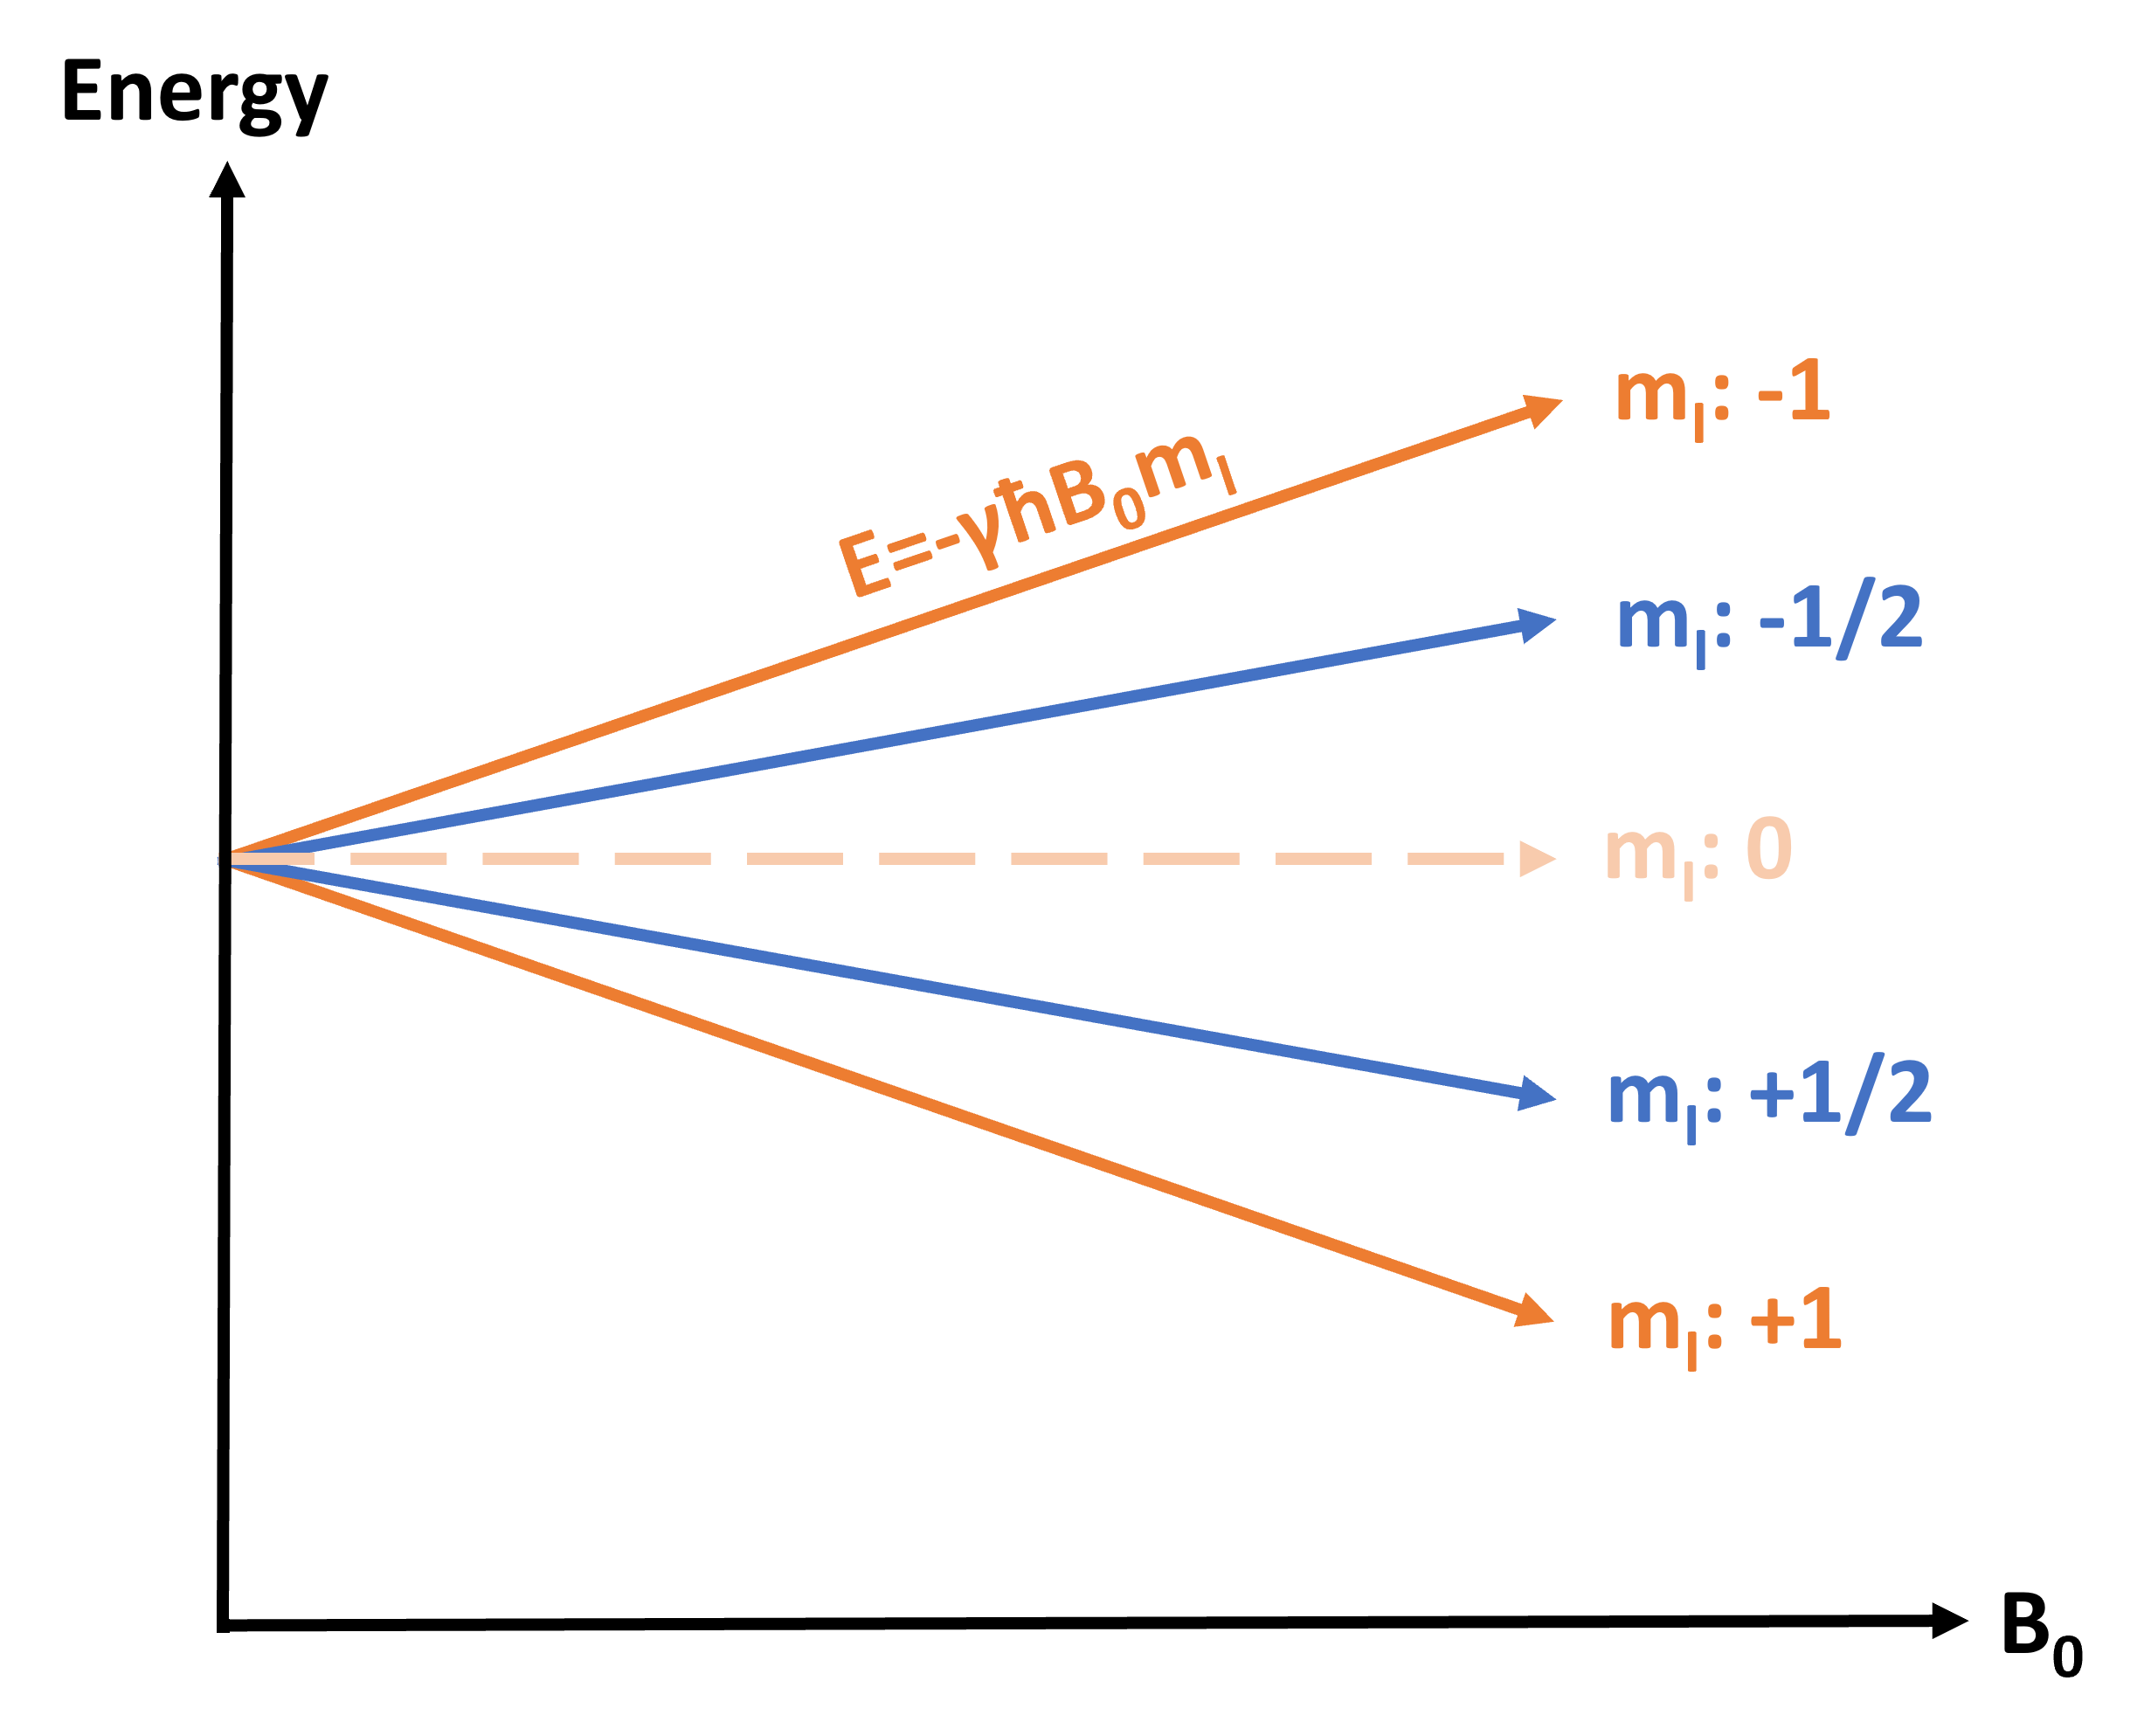
\includegraphics[width=0.8\textwidth]{Figures/Theory/Zeeman.png}
    \caption{\textit{Figure demonstrating the change in spin energy levels due to increasing magnetic field B$_0$, for spin-1/2 and spin-1 nuclei. Demonstrating the Zeeman Effect \cite{Zeeman1896VerslagenAfdeeling}.}}
    \label{fig:theory:zeeman}
\end{figure}

This gives a good overview of how individual spins act and behave in magnetic fields, however our bodies contain a collection of spins of different nuclei. Therefore, it is important to apply these relationships to a collection of spins which will give an overview of macroscopic behaviours that make up the theory of \ac{NMR}.

\subsection{Macroscopic Behaviour}

The molecules of interest for \ac{MRI} are in the liquid state which means the motion of the spin is largely random and due to Brownian motion, thermal energy then becomes the dominant driving force and therefore quantum effects become negligible. When particles have a large enough temperature ($T$) and there are enough particles, the distribution over multiple energy levels can be described according to the Boltzmann distribution \cite{Boltzmann1872WeitereGasmolekulen}. Equation \ref{eqn:theory:boltz} empirically states the probability $p$ of a single particle being in a specific state.

\begin{equation}
    p_i = \frac{\exp\left(\frac{E_i}{k_BT}\right)}{\displaystyle \sum_{j = 1}^{M}\exp\left(\frac{E_j}{k_BT}\right)}
    \label{eqn:theory:boltz}
\end{equation}

Where $i$ indicates the specific energy levels and $M$ is the total number of available states for a specific nuclei. The overall magnetic field that results from a large group of spins can be described by a vector called magnetisation ($M$). Most of the spins contributions will cancel so the only contribution to the magnetisation vector arises from the difference in the number of energy levels. A generalised summation that calculates the equilibrium magnetisation is shown in equation \ref{eqn:theory:mag}.

\begin{equation}
    M = N\sum_{j = 1}^{M}p_j\mu_j
    \label{eqn:theory:mag}
\end{equation}

Where $N$ is the number of spins of interest. A more simplified version of equation \ref{eqn:theory:mag} that is still general to all spins is empirically shown in equation \ref{eqn:theory:mag_s}.

\begin{equation}
    M = \frac{s(s+1)\gamma^2 \hbar^2 N B_0}{3k_BT}
    \label{eqn:theory:mag_s}
\end{equation}

A major assumption that is made to get to this point which is that the thermal energy at room temperature is much larger than the nuclear magnetic energies. Most fundamental particles and most nuclei that are of interest for \ac{NMR} are spin-1/2, which give two distinct energy levels. So in order to simplify the magnetisation calculations only the spin-1/2 nuclei are considered. Equation \ref{eqn:theory:mag_1H} calculates the magnetisation for spin-1/2 nuclei.

\begin{equation}
    M = \frac{\gamma^2 \hbar^2 N B_0}{4k_BT}
    \label{eqn:theory:mag_1H}
\end{equation}

Magnetisation is largely responsible for the signal produced in \ac{NMR} experiments, which is proportional to the total number of spins inversely proportional to temperature (measured in kelvin). The temperature will mostly remain constant for experiments performed in humans \textit{in vivo} at room temperature (except for hyperpolarisation). Also, $M$ is proportional to the magnitude of any applied external magnetic field applied ($B_0$) this is because the fields applied in \ac{NMR}/\ac{MRI} are on the scale of Tesla's or 10's of Tesla (T) whilst earth's magnetic field is on the scale of 5x10$^{-5}$T, therefore magnetisation due to earth's field is often considered zero. Therefore, all the magnetic moments will be pointing in random directions which is why they cancel. When $B_0$ is applied the orientation of the spins still remains random and Brownian, however a bias will be present which generates the overall magnetisation of the collection of spins. This alone is not enough for \ac{NMR}/\ac{MRI} to develop on the scale as it has, in order to receive vital \textit{in vivo} information of the human body it is important to manipulate magnetisation \cite{Haacke2014MagneticDesign}. 

\subsection{Manipulating Magnetisation}

\begin{figure}
    \centering
    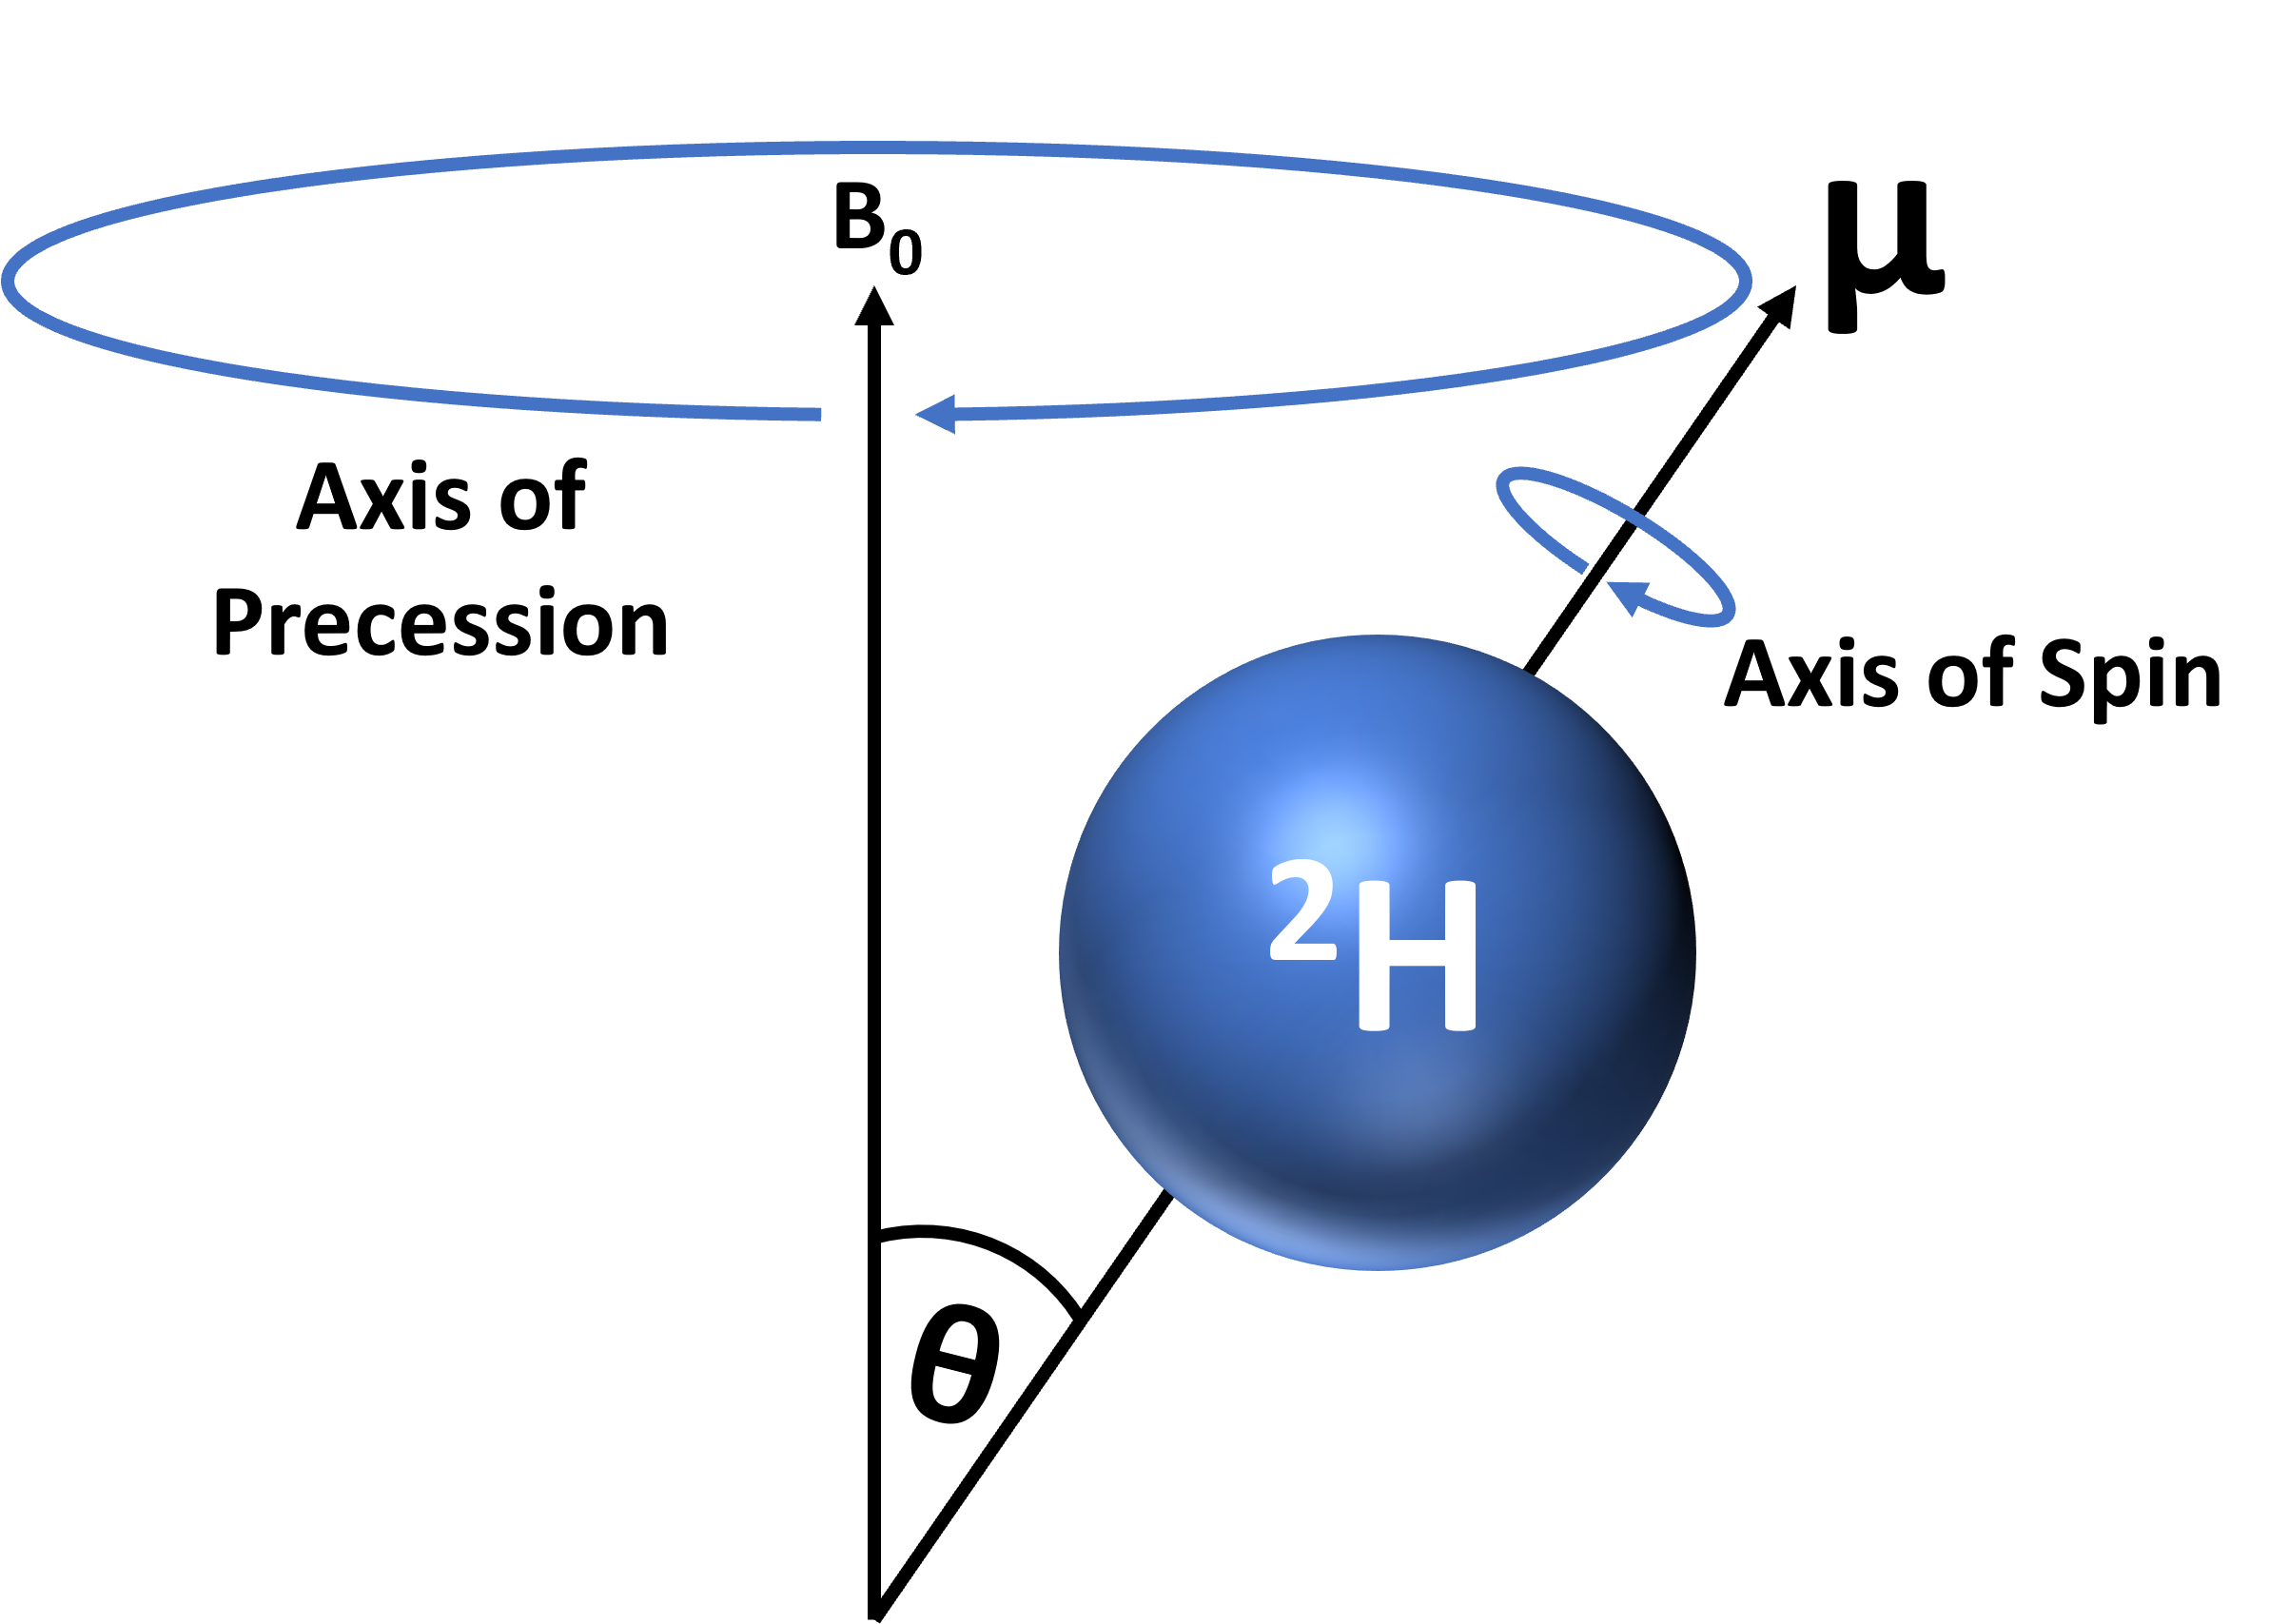
\includegraphics[width=0.9\textwidth]{Figures/Theory/Moment.png}
    \caption{\textit{A diagram of a $^2$H nuclei spinning and precessing around an applied external magnetic field B$_0$, its magnetic moment $\mu$ and both axis are labelled along with the angle the magnetic moment vector makes to B$_0$.}}
    \label{fig:theory:moment}
\end{figure}

The overall direction of the magnetisation vector is the in the same direction as the applied field. Magnetisation is made up of two main components, the longitudinal and the transverse. The longitudinal is the component that is parallel to the applied field, with the transverse being a combination of the two other orthogonal directions. Often the applied field, and analogously the magnetisation, is given as $\mathbf{B}=B_0\mathbf{z}$ and therefore the longitudinal component is the z-direction, which makes the transverse component a combination of the x and y component. This means that the transverse magnetisation (M$_{xy}$) during the applied field is zero. After a large enough period of time of an applied field the magnetisation  will reach the value outlined in equation \ref{eqn:theory:mag_1H} (M$_0$). The total evolution of the magnetisation including the longitudinal and transverse components is referred to as the Bloch equation \cite{Bloch1946NuclearInduction}.

\begin{equation}
    \frac{d\mathbf{M}}{dt} = \, \gamma\mathbf{M}\textrm{x}\mathbf{B} \, + \, \frac{M_0-M_z}{T_1}\mathbf{z} \, - \, \frac{\mathbf{M_{xy}}}{T_2}
    \label{eqn:theory:Bloch}
\end{equation}

The first term in equation \ref{eqn:theory:Bloch} describes the change in magnetisation according to the Larmor frequency. The second term describes how the longitudinal magnetisation reaches steady state value during a static applied field in the z-direction (parallel to the field), where T$_1$ is the longitudinal or spin-lattice relaxation time constant and results from the spins interaction to its surrounding lattice. The final term shows how the transverse magnetisation returns back to zero if an applied field is applied in the transverse plane, where T$_2$ is the transverse or spin-spin relaxation time constant and arises from dephasing due to each spins interaction to its neighbouring spins. 

The transverse relaxation time is outlined here in the perfect case where the field applied is perfectly homogenous, however in reality this is rarely the case. This alters the time constant such that it is now T$_2^*$.

\begin{equation}
    \frac{1}{T_2^*} = \frac{1}{T_2} + \frac{1}{T_2^{'}}
    \label{eqn:theory:trans}
\end{equation}

Where T$_2^{'}$ is dependent only on the homogeneity of the field, this means that technically T$_2^*$ can change between scans and scanners ect. Realistically T$_2^*$ does not vary much between cases. The relaxation times T$_1$ and T$_2^*$ are specific for each nuclei, tissue type and field strength. In spectroscopy the \ac{FWHM} of each signal/peak is related to the total transverse relaxation (\ac{FWHM}$ = 1 / \pi T_2^*$). The Bloch equation can then be separated for each component ($x,y,z$) and made specific for each experiment, for example there is the static field case substituting $\mathbf{B}=B_0\mathbf{z}$, or it is possible to flip the magnetisation into the transverse plane using $\mathbf{B}=B_0\mathbf{z}+B_1\mathbf{x}$. 

\begin{figure}
    \centering
    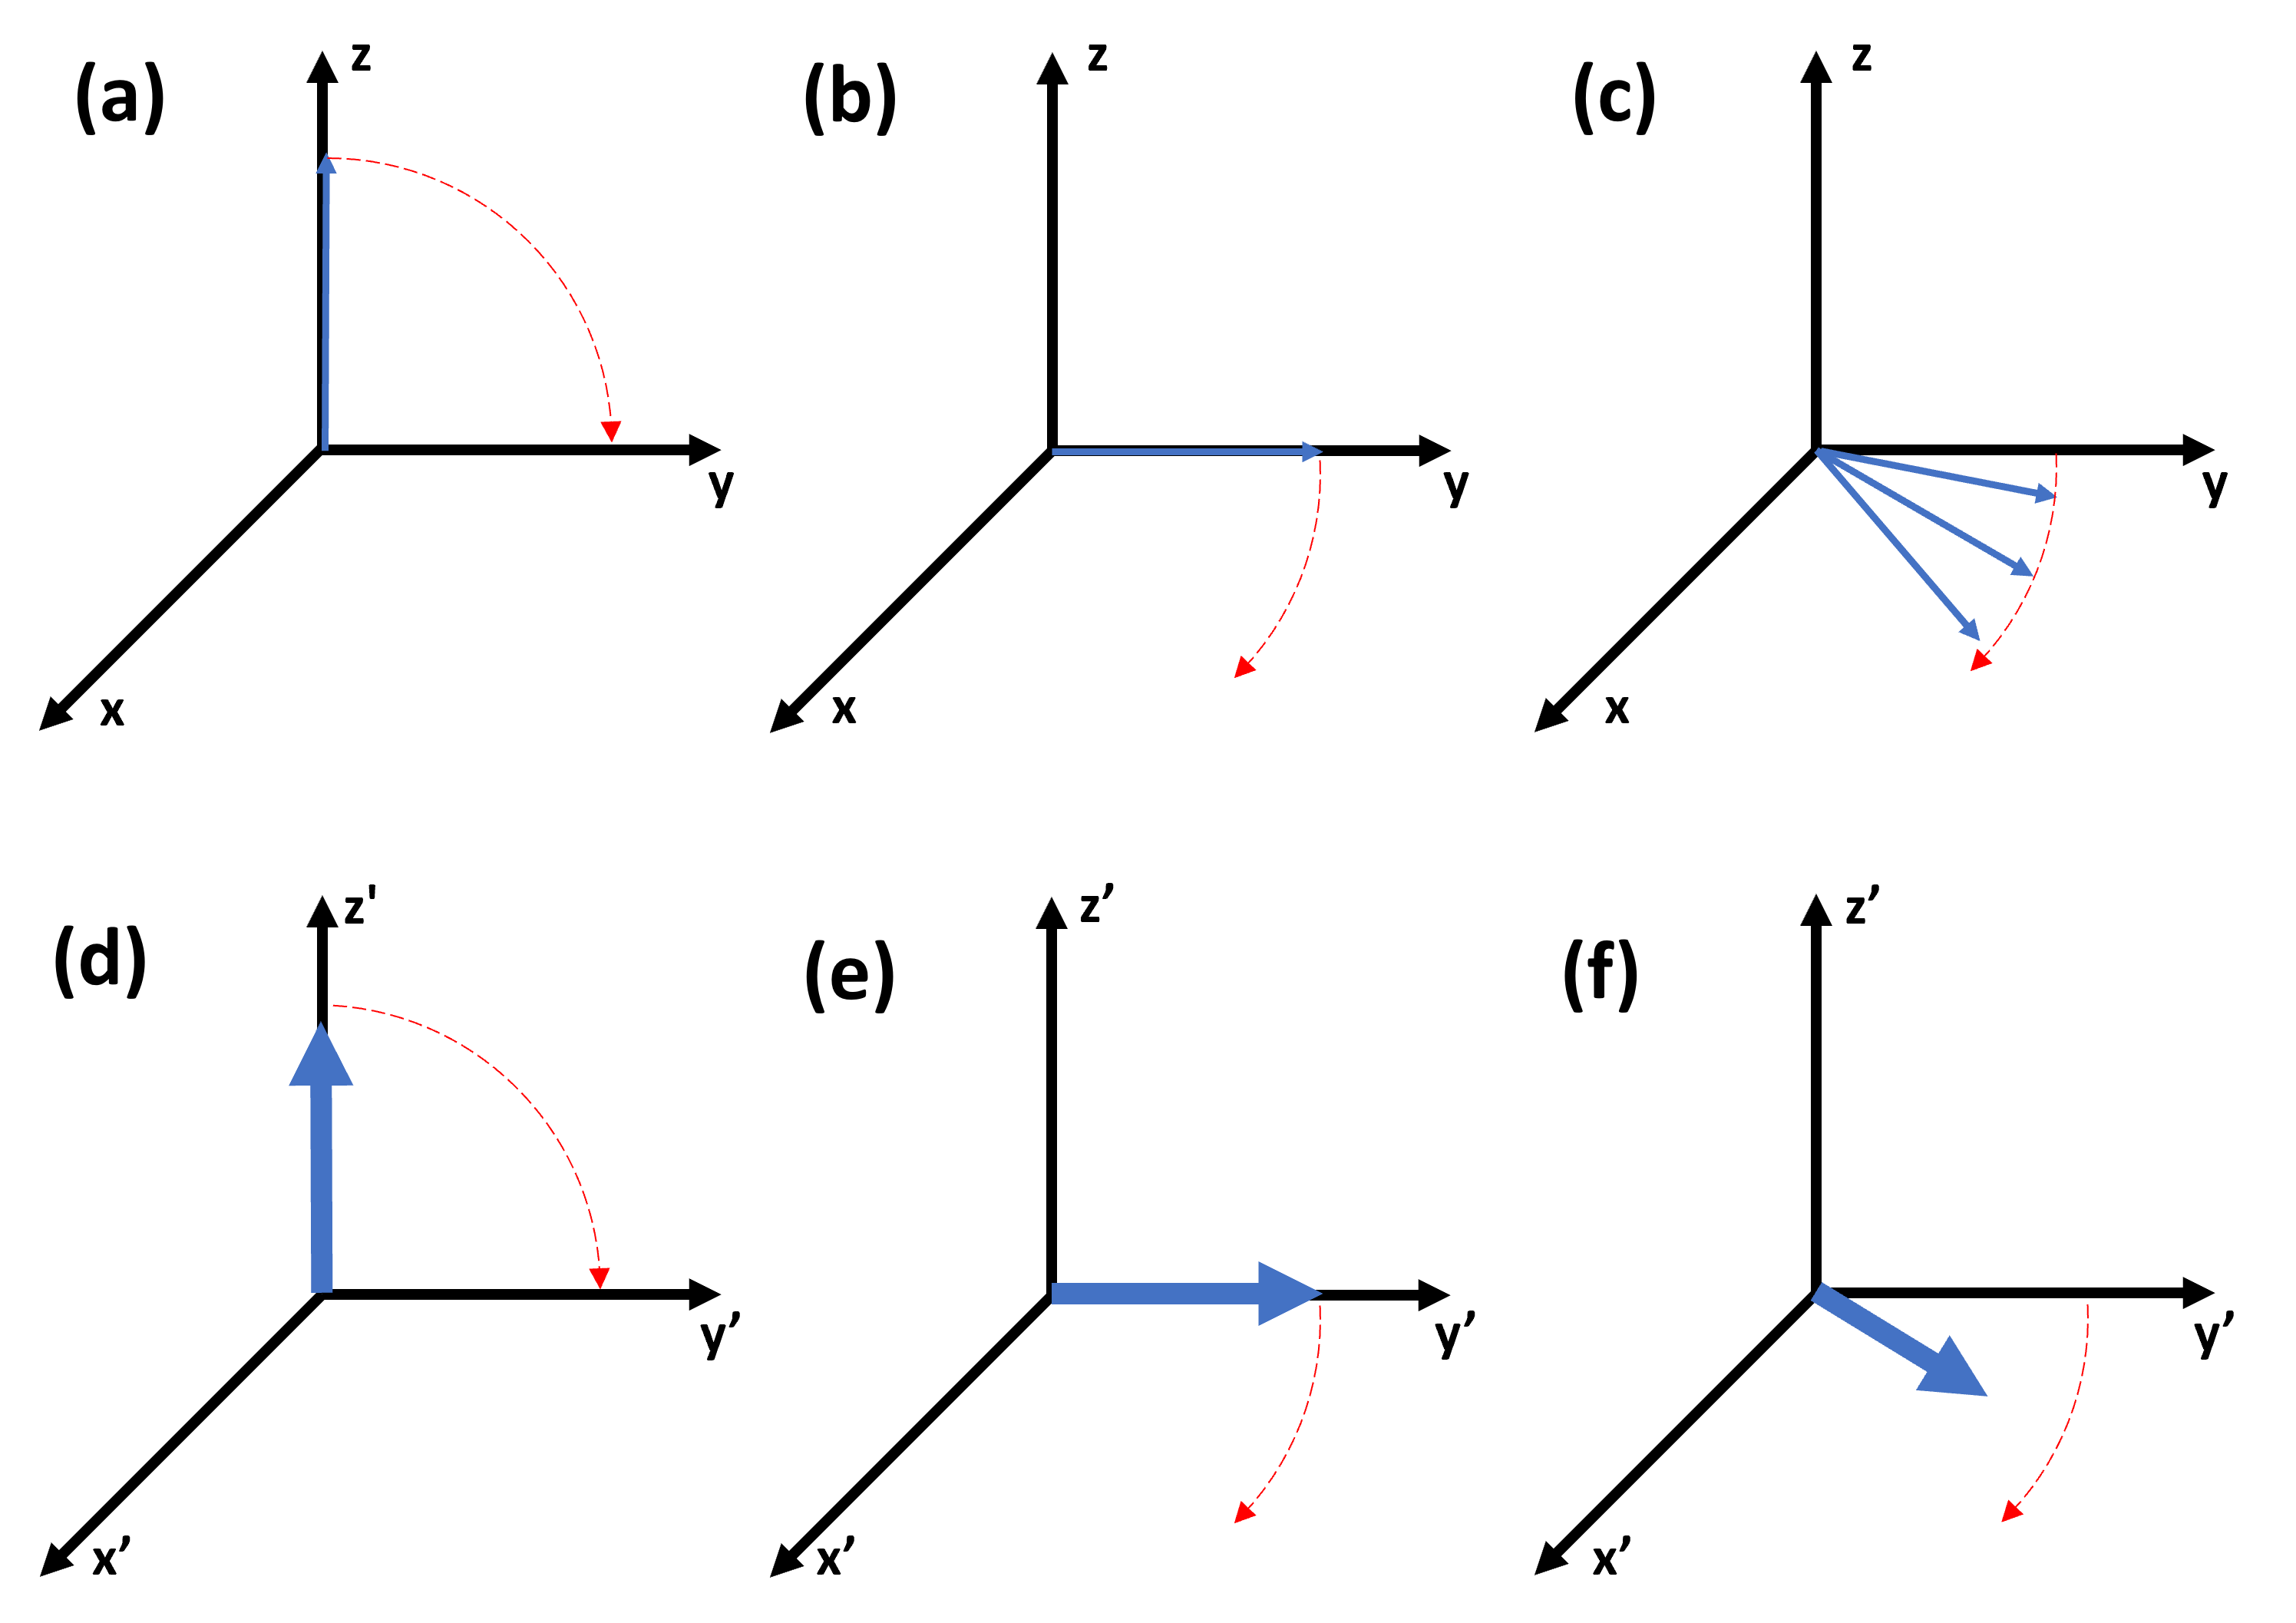
\includegraphics[width=0.9\textwidth]{Figures/Theory/Magnetisation.png}
    \caption{\textit{Diagram visually showing the effect of applied external magnetic fields on magnetic moment vectors and magnetisation.(a) Shows the precession of a collection of magnetic moment vectors after a static magnetic field (B$_0$) is applied the z-direction, and just before a 90$^\circ$ degree pulse (B$_1$) is applied in and B$_0$ is removed. (b) Here the magnetic moments have been tipped to all align in the positive y-direction following an applied B$_1$ pulse. (c) Now the pulse has been removed and the spins begin to dephase according to transverse relaxations with the time constant T$_2^*$. With the spins 'fanning' out in the x-y plane until no overall transverse magnetisation is left and the spins return to random orientations. (d-f) Follow show the spins experiencing the same B$_0$ and B$_1$ as in (a-c) except now only the overall Magnetisation vector is shown in the rotating reference frame. It is important to note the spins do not experience longitudinal relaxation as B$_0$ has already been turned off and is 0 in the x-y plane, if B$_0$ was still applied spins would return to the orientations in (a,d), therefore the diagram only demonstrates transverse relaxation.}}
    \label{fig:theory:Mag}
\end{figure}

The precession of magnetisation can be difficult to conceptualise/visualise in a stationary reference frame due to the complex 3D motion. Therefore it is beneficial to consider the system in a rotational reference frame ie. as if the observer rotates around the z-axis. The common reference frame used is one that rotates at the same frequency as the applied B$_1$ frequency ($\gamma B_1$) around the z-axis. This gives the following separated Bloch equations for the variation of magnetization in each orthogonal axis ($x',y',z$) in the reference frame, for a left-circularly polarised \ac{RF} field B$_1$ which is parallel to $x'$ in the rotating frame.

\begin{equation}
    \frac{dM_{x'}}{dt} = \Delta\omega M_y^{'} - \frac{M_x^{'}}{T_2}
    \label{eqn:theory:Blochx}
\end{equation}
\begin{equation}
    \frac{dM_{y'}}{dt} = \Delta\omega M_x^{'} + \omega_1M_z^{'} - \frac{M_y^{'}}{T_2}
    \label{eqn:theory:Blochy}
\end{equation}
\begin{equation}
    \frac{dM_z}{dt} = -\omega_1M_y^{'} + \frac{M_0-M_z^{'}}{T_1}
    \label{eqn:theory:Blochz}
\end{equation}

Here, $\Delta\omega$ is the difference between the Larmor frequency ($\omega_0$) and the frequency of the rotating reference frame ($\omega$), and represents any off resonance effects. Therefore, if the reference frame rotates at the Larmor frequency these terms disappear. If only the static field case wants to be considered the $\omega_1$ terms disappear as well which leaves only the relaxation dominant terms. If short-lived pulses are considered where $\omega_1$ is much larger than 1/T$_1$ and 1/$T_2$ the solutions to equations \ref{eqn:theory:Blochx} - \ref{eqn:theory:Blochz} are given as follows.

\begin{equation}
    M_{x'}(t) = \exp(-t/T_2) \left( M_{x'}(0)\cos\Delta\omega t \, + \, M_{y'}(0)\sin\Delta\omega t \right)
\end{equation}
\begin{equation}
    M_{y'}(t) = \exp(-t/T_2) \left( M_{y'}(0)\cos\Delta\omega t \, + \, M_{x'}(0)\sin\Delta\omega t \right)
\end{equation}
\begin{equation}
    M_z(t) = M_z(0)\exp(-t/T_1) \, + \, M_0 \left( 1-\exp(-t/T_1) \right)
\end{equation}

The \ac{NMR} signal arises from the longitudinal magnetisation, however this is very small and can be dominated by magnetisation from electron currents within atoms and molecules. Therefore the magnetisation is often tipped into the transverse plane where it is in the same plane as the precession and will therefore induce current in a receiver coil, at the Larmor frequency. In between short applied fields (\ac{RF} pulses) it is therefore important to wait a large enough period of time for the transverse signal to relax back into its longitudinal state before repeating the process to acquire more data. Therefore, whilst the longitudinal magnetisation is important for overall signal it is important to accurately and reliably tip the magnetisation exactly at 90$^\circ$, as deviations in this 'flip-angle' ($\theta$) could reduce the available signal \cite{deGraaf2019InSpectroscopy}.

\subsection{Flip Angles, Phase and Signal}

The flip angle ($\theta$) generated from a short, finite \ac{RF} pulse applied (excitation) is dependent on the B$_1$ magnetic field and the duration that the pulse is turned on for ($\tau$) according \ref{eqn:theory:FA}.

\begin{equation}
    \Delta\theta = \gamma B_1 \tau
    \label{eqn:theory:FA}
\end{equation}

Where $\theta$ is the angle after excitation to the longitudinal z-axis, also known as the flip-angle. The closer this is to 90$^\circ$ the larger the contribution of longitudinal signal is transferred into the transverse plane. The precessing transverse signal is said to be a complex signal such that $f(t) = R(t) + I(t)$, this is known as a \ac{FID} and is the signal induced in the receiver coil.

\begin{equation}
    R(t) = M_0\cos(\omega t+ \phi)\exp(-t/T_2^*)
    \label{eqn:theory:real}
\end{equation}
\begin{equation}
    I(t) = -M_0\sin(\omega t+ \phi)\exp(-t/T_2^*)
    \label{eqn:theory:imag}
\end{equation}

Where $\phi$ is the phase of the signal and represents the angle the transverse magnetisation makes to the $x'$ axis after excitation, i.e a phase of -90$^\circ$ would be aligned parallel to the y-axis. The parameters that depend on the total signal from equations \ref{eqn:theory:real} and \ref{eqn:theory:imag} ($M_0, \, \omega, \, \phi \, \textrm{and} \, 1/T_2^*$) represent the parameters that were mentioned in the previous section (Amplitude, frequency, phase and linewidth) respectively. The real and imaginary components can be combined using Euler's formula to give equation \ref{eqn:theory:euler}. This signal is currently in the time-domain and therefore is difficult to separate different frequency contributions from the signal. Therefore, it is important to change this signal to be in the frequency domain spectrum which can be done using a \ac{FT} \cite{Fourier1822TheorieChaleur}, the equation used for doing this is shown in equation \ref{eqn:theory:fourier}.

\begin{figure}
    \centering
    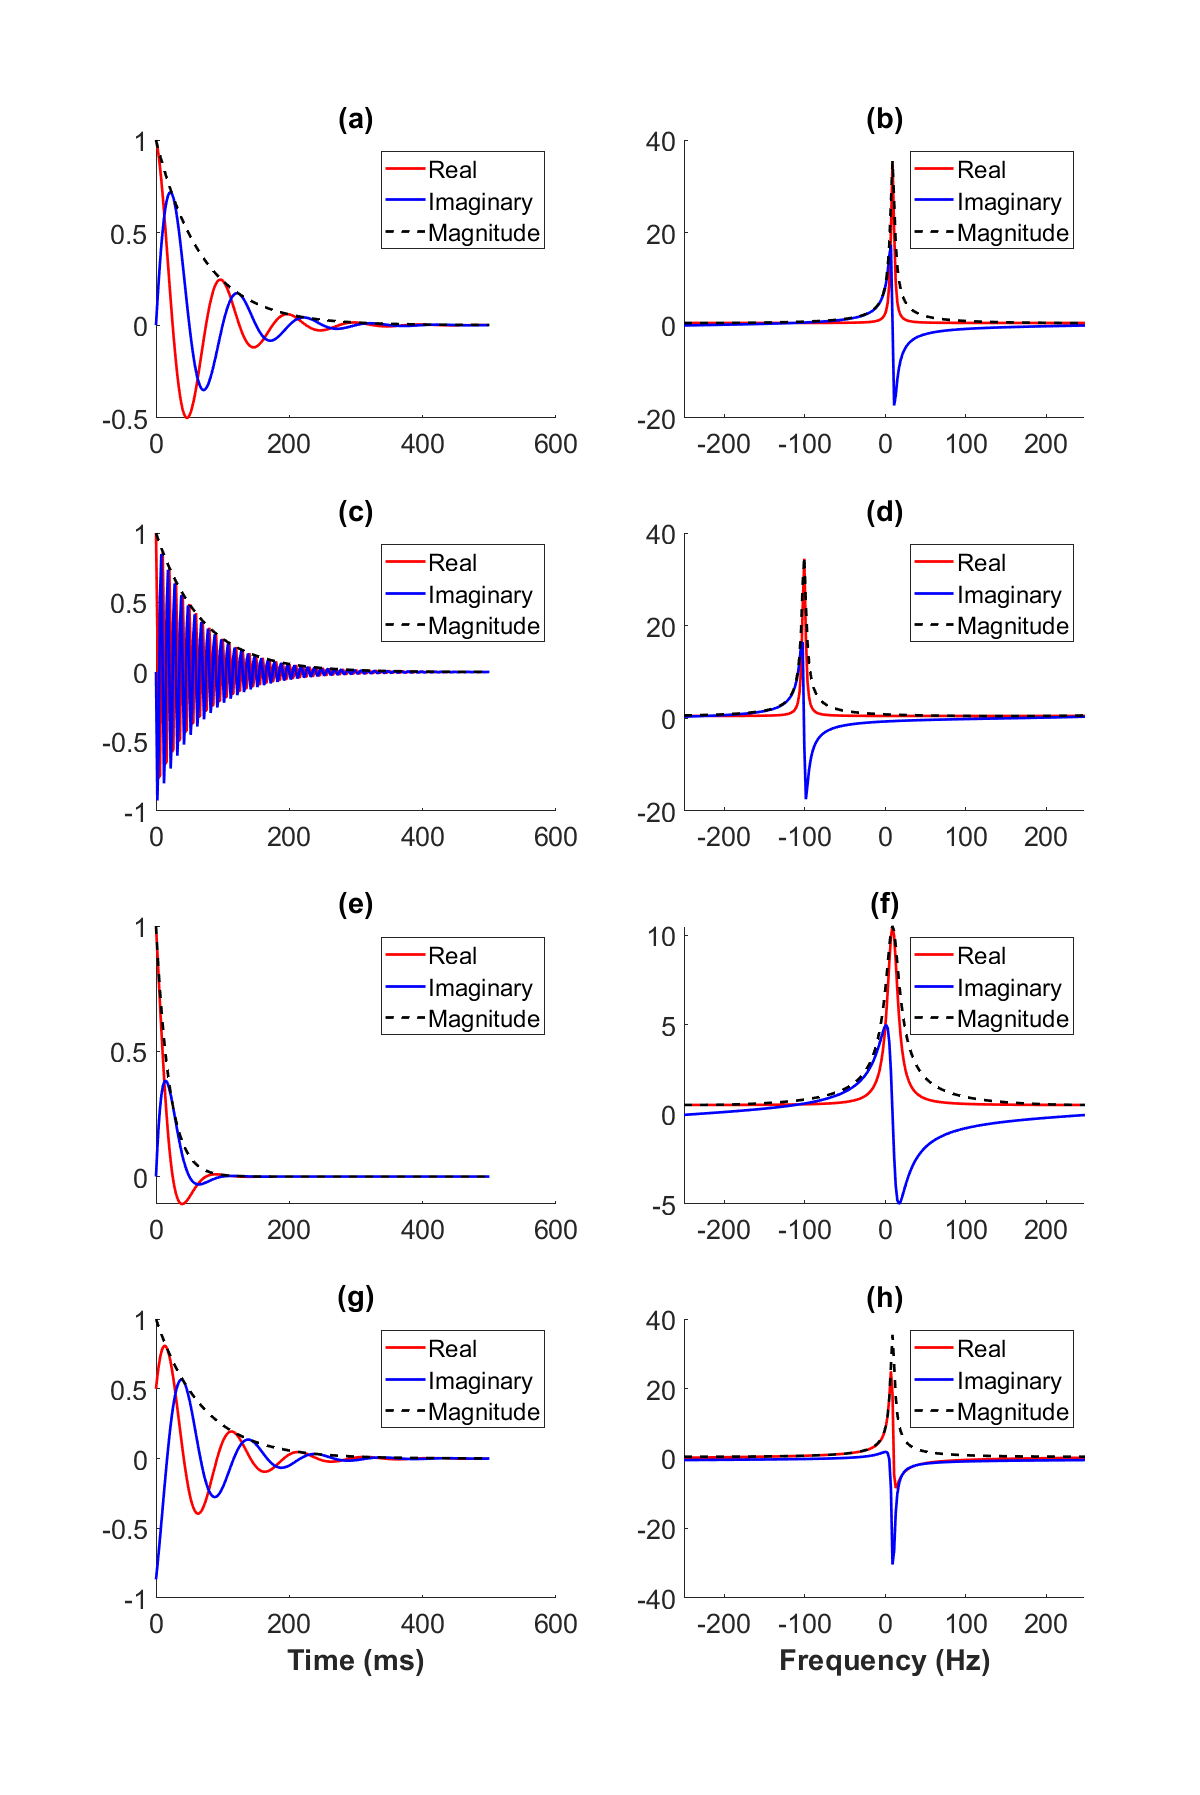
\includegraphics[width=0.9\textwidth]{Figures/Theory/FID_Lorentz.png}
    \caption{\textit{Graphs of \ac{FID}'s (left) and corresponding lineshapes (right) for different frequency offsets ($\nu_0$), transverse relaxation times (T$_2^*$) and phases ($\phi$), all graphs have an amplitude ($A$) of 1. The parameters for (a) and (b) are $\nu_0$=-10 Hz, T$_2^*$= 70 ms and $\phi$=0, each row then changes one parameter each. (c) and (d) have a different $\nu_0$ of +100 Hz. (e) and (f) have a shorter T$_2^*$ of 20 ms. (g) and (h) have a lower phase of $\phi$=-$\pi$/3.}}
    \label{fig:theory:FID_Lorentz}
\end{figure}

\begin{equation}
    f(t) = M_0\exp(-2\pi i \nu_0t)\exp(-t/T_2^*)\exp(i\phi)
    \label{eqn:theory:euler}
\end{equation}

\begin{equation}
    F(\nu) = \int_{-\infty}^{+\infty} f(t)\exp(-2\pi i \nu t) \, dt
    \label{eqn:theory:fourier}
\end{equation}

Where $F(\nu)$ is the new frequency domain spectrum, $\nu$ is the frequency , $f(t)$ is the time domain signal which in this case is the \ac{FID}. By applying a \ac{FT} to the \ac{FID} equation \ref{eqn:theory:lorentz} is obtained, which depends on the same four parameters as the \ac{FID}. The relationship between the T$_2^*$ and the FWHM has already been shown, therefore as the T$_2^*$ gets longer the wider the peak becomes. It is important to note that the integral/area under the peak remains the same for changes in T$_2^*$ as it depends on the amplitude (A). Therefore, the shorter the T$_2^*$ the larger the peak height and \textit{vice versa}, and therefore maximising A and minimising T$_2^*$ maximises the available \ac{SNR} in the spectrum.

\begin{equation}
    F(\nu) = A\exp(i\phi)\frac{R_2^*-i2\pi(\nu-\nu_0)}{R_2^{*2}+4\pi^2(\nu-\nu_0)^2}
    \label{eqn:theory:lorentz}
\end{equation}

Using \ac{NMR} to measure signals from pure samples with only one nuclei present will produce spectra with single peaks and therefore is a great way to measure magnetic moments of different nuclei. However, when using \ac{NMR} \textit{in vivo} like with \ac{MRS} all molecules and tissues are complex and consist of multiple different nuclei bound in multiple different ways. The shielding of the magnetic field at the nucleus by surrounding electron cloud changes the magnetic field at the nucleus, this changes the resonant frequency of precession for nuclei. Therefore, nuclei that have different chemical environments will have different frequencies which means that the \ac{NMR} signal will be at different frequency positions in a \ac{NMR} spectra. Therefore by looking at where peaks are in an \ac{NMR} spectra and the amplitude of the peaks it is possible to find out about the chemical structure of the tissue/compound being investigated which is useful in studies of medical conditions and diseases. The main unit of measure for frequency is hertz (Hz), however the values here will change greatly depending on the nuclei of interest and the field strength being used. Therefore a new quantity and unit of measure is often used for the frequency in NMR/\ac{MRS} spectra to make it much more generalised and therefore applicable to all nuclei and field strengths, it is known as chemical shift ($\delta$) and is measured in parts-per-million (ppm). The equation to calculate chemical shift from frequency is shown in equation \ref{eqn:theory:chemshift}.

\begin{equation}
    \delta = \frac{\nu - \nu_{\textrm{ref}}}{\nu_\textrm{ref}} \, \textrm{x} \, 10^6
    \label{eqn:theory:chemshift}
\end{equation}

So far it has been outlined how to obtain an \ac{NMR} signal in samples and in the body using MRS. However, sometimes it is not enough to just obtain information on the chemical structures/composition of the body and spatial information is needed to obtain chemical compositions of specific areas in the body. The most common way to do this is to use magnetic fields that vary spatially \cite{Haacke2014MagneticDesign}. 

\subsection{Introduction of Gradients}

According to equation \ref{eqn:theory:Lamor} the frequency of precession is dependent on the magnetic field applied, therefore if a magnetic field varies in the any direction (G$_{slice}$) the frequency of precession will also vary in said direction. Previously, if only a static spatially-homogeneous B$_0$ was applied to a sample and an \ac{RF} pulse is used to tip the magnetisation all the spins in that sample will be tipped, however if G is applied along with B$_0$ only the spins with the same frequency (where G$_{slice}$=0) as the \ac{RF} pulse will be tipped. The new magnetic field applied empirically will appear like equation \ref{eqn:theory:B_Grad}, with the frequency that is spatially dependent is shown in equation \ref{eqn:theory:f_Grad}.

\begin{equation}
    B(r) = B_0 \, + \, Gr
    \label{eqn:theory:B_Grad}
\end{equation}

\begin{equation}
    \nu(r) = \gamma(B_0 \, + \, Gr)
    \label{eqn:theory:f_Grad}
\end{equation}

Here $r$ is used to represent any direction. Therefore only a spatially localised 'slice' will be excited and any signal received will be specifically from that slice. By changing the frequency of the pulse applied means that a different slice can be applied. If the pulse contains a range of frequencies (bandwidth) all the frequencies in the bandwidth will be excited, this results in a slice being excited that has a physical thickness. If this process is repeated spectra can be acquired from multiple slices and therefore the changes in signals can be compared to position in the body of which the slice was acquired. The link between magnetic field/frequency and position using gradients is demonstrated visually in Figure \ref{fig:theory:Grad}.

\begin{figure}
    \centering
    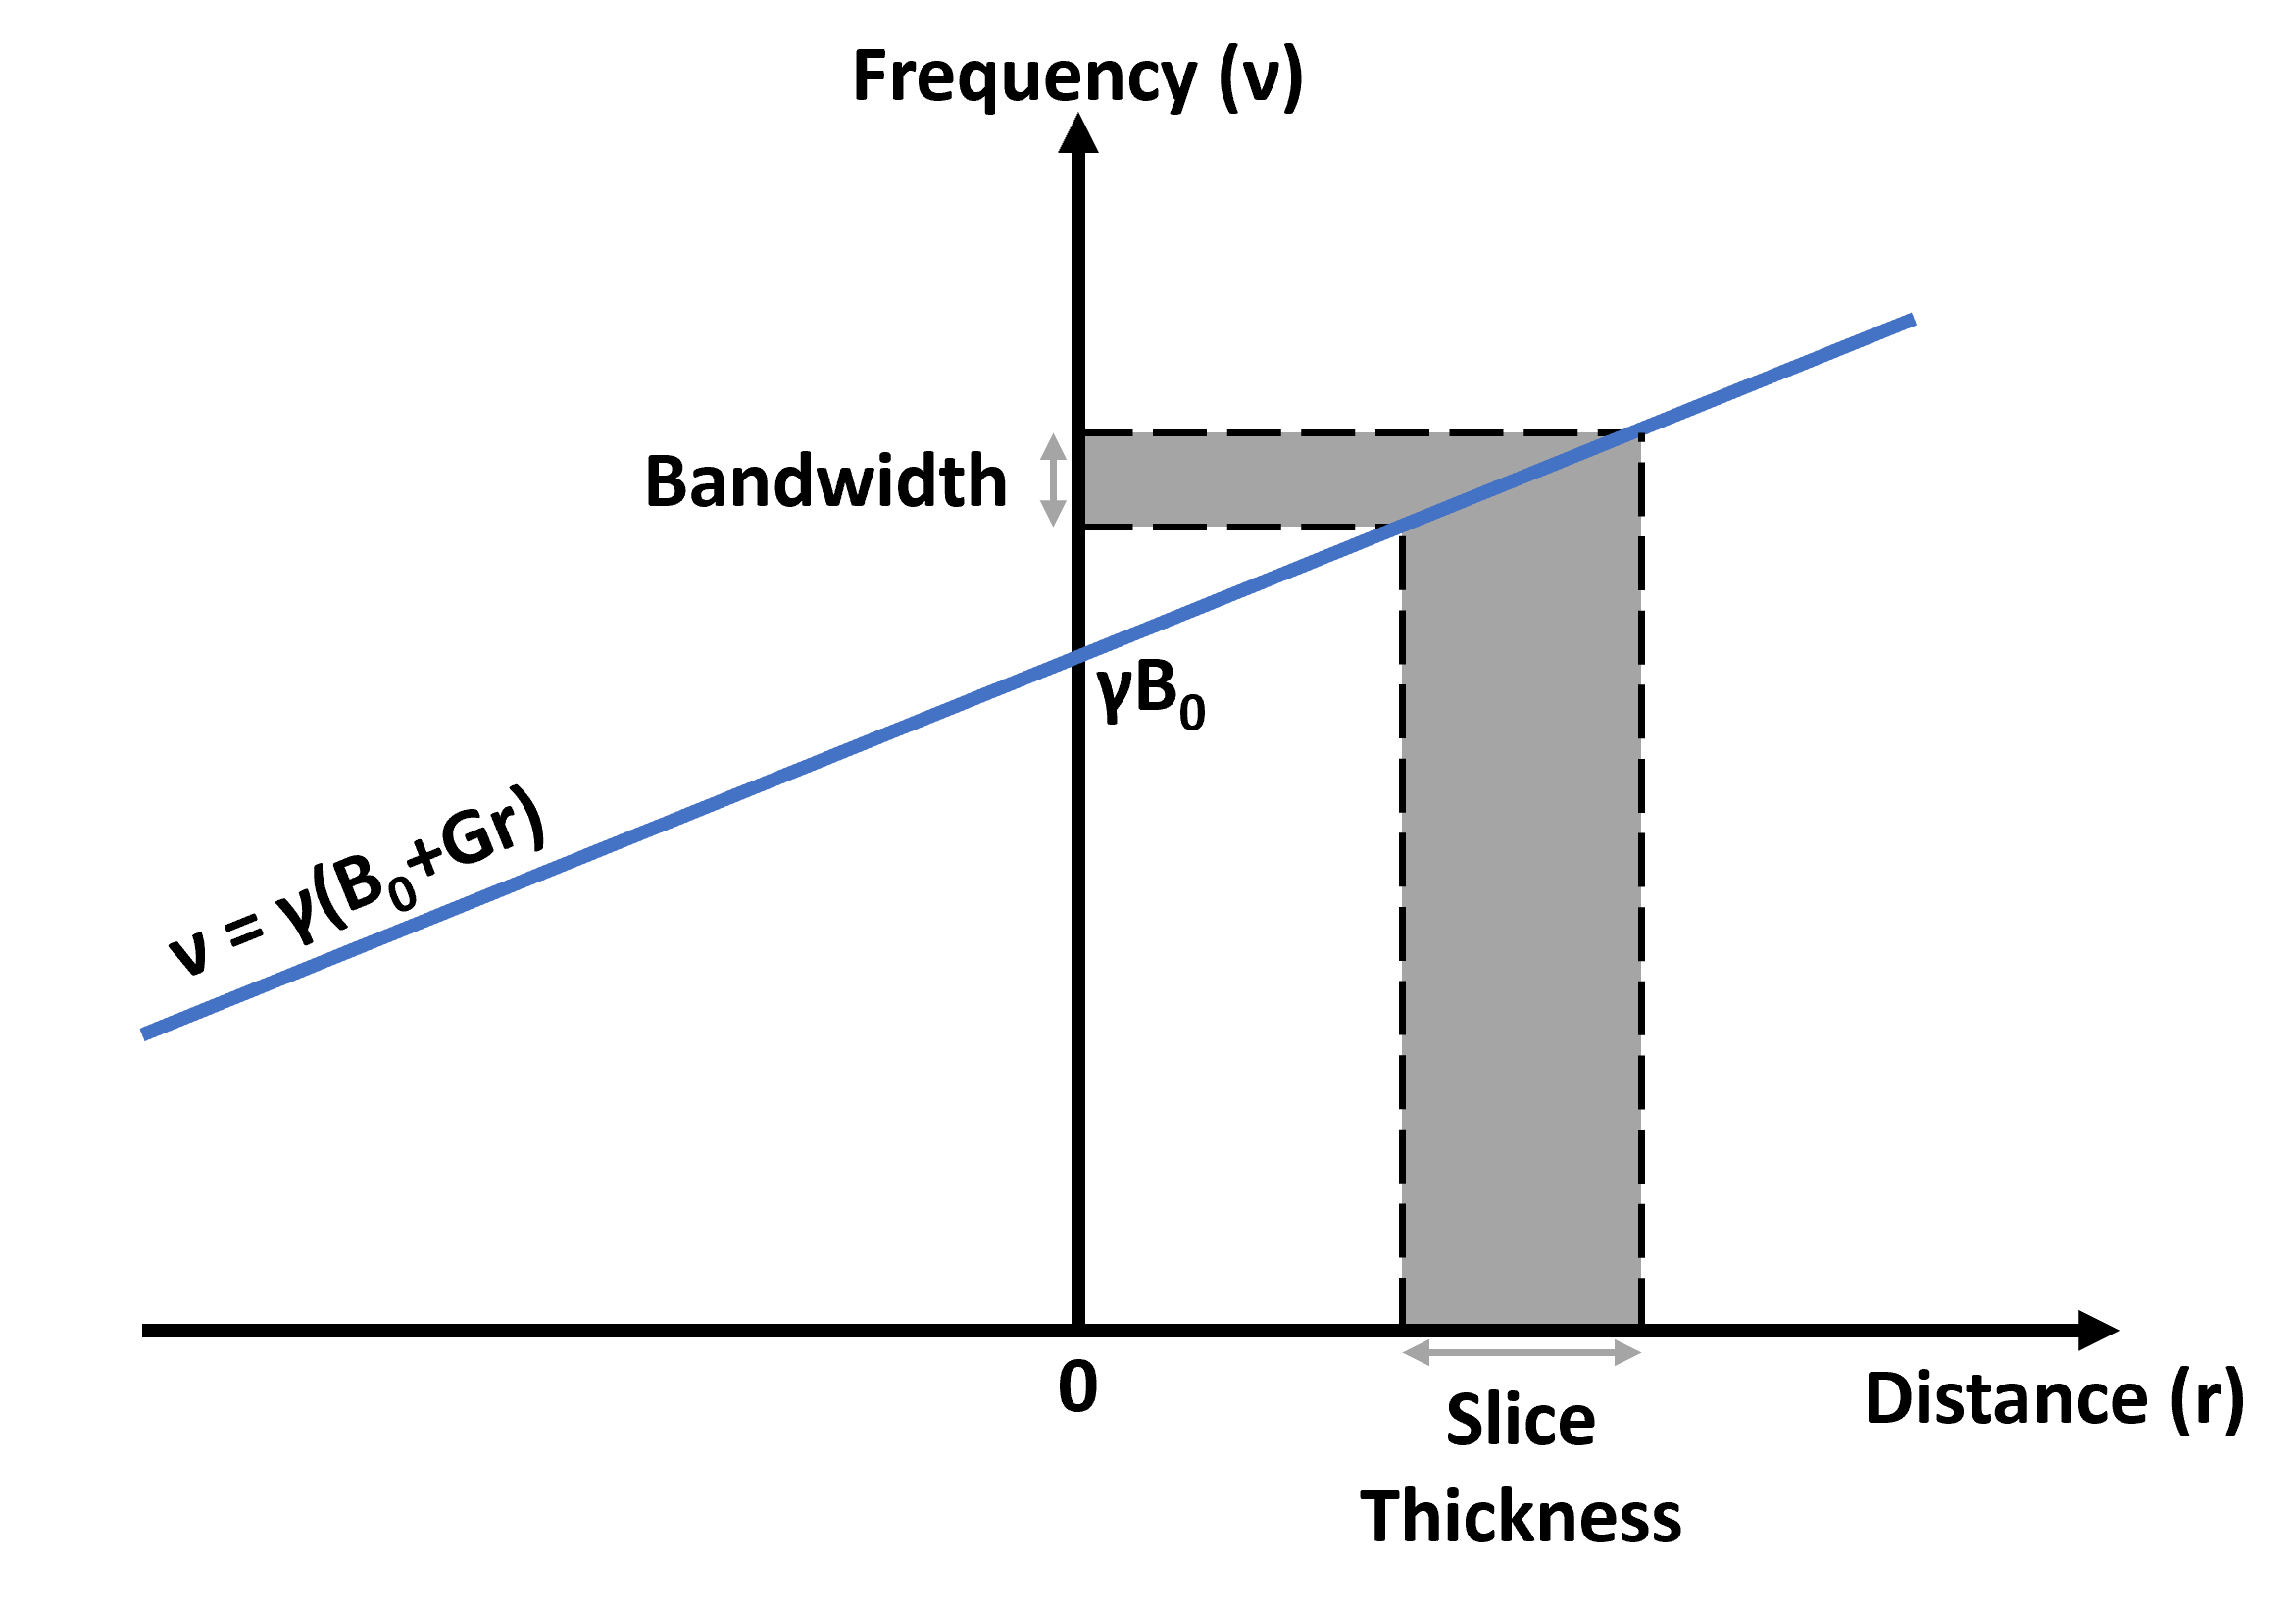
\includegraphics[width=0.9\textwidth]{Figures/Theory/Gradient.png}
    \caption{\textit{The analogy between frequency of precession ($\nu$) and thickness of an acquired slice when a gradient ($G_{slice}$) is applied. This works for all directions, but is most commonly applied in the z-direction.}}
    \label{fig:theory:Grad}
\end{figure}

\ac{RF} coils are used to generate these pulses and often the frequency that the pulse generates is more difficult to change than it is to change the gradient, therefore if this process is repeated often its the gradient that changes not the \ac{RF} frequency. If the chemical composition of what is being investigated is not important it is possible to acquire entirely spatial information and create a volumetric image based on multiple slices. To do this more gradients are needed than just the slice-selective gradient \cite{deGraaf2019InSpectroscopy}.

\section{Differences for $^2$H}

Deuterium ($^2$H) is the only stable isotope of hydrogen ($^1$H), the nucleus of a $^2$H atom is called a deuteron and There are no such natural processes that produce large levels of $^2$H other than the Big Bang Nucleosynthesis which starts with the production of $^2$H, as $^2$H is destroyed very quickly in star's fusion \cite{Patrignani2016ReviewPhysics}. The $^2$H abundance found on earth's ocean has been found to be similar to what has been found in comets, which adds evidence that ocean water originates from comets \cite{Hersant2001APlanets}. Most of the natural $^2$H content arises as \ac{HDO} in water, the $^2$H content of different water sources (oceans, rainwater etc) are used to track the water cycle \cite{Bowen2019IsotopesApplications}. This leads to our bodies having a very low \ac{NA} $\approx$0.015\% of $^2$H, which makes $^2$H appealing for tracer studies as small concentration increases are easy to detect above baseline. The addition of a neutron to the nucleus of $^2$H means the gyromagnetic ratio ($\gamma$) is smaller than that of $^1$H (6.54 vs 42.6 MHzT$^{-1}$) which reduces the Larmor frequency of $^2$H according to equation \ref{eqn:theory:Lamor}. $^2$H has an integer spin of 1 and due to the non-symmetric distribution of charge within the nucleus has a quadrupolar magnetic moment of 0.286 fm$^2$, as the quadrupolar moment interacts with local electric field which induces extra relaxation, this reduces both the longitudinal and transverse relaxation times. The integer spin also introduces an extra energy level more than for $^1$H with the available spin values of $m_s$ = -1, 0 and 1. Considering magnetisation is the net vector sum of $\mathbf{\mu}$ the net magnetisation is due to the population differences between the lowest and largest energy levels. Using equation \ref{eqn:theory:mag} and/or \ref{eqn:theory:mag_s} a simplified equilibrium magnetisation can be found, which is shown in equation \ref{eqn:theory:mag_2H}.

\begin{equation}
    M = \frac{2\gamma^2 \hbar^2 N B_0}{3k_BT}
    \label{eqn:theory:mag_2H}
\end{equation}

Whilst the magnetisation appears to be 8/3 larger for $^2$H compared to $^1$H in equation \ref{eqn:theory:mag_2H}, it is important to remind the reader that it is dependent on the gyromagnetic ratio squared along with the number of spins. The gyromagnetic ratio squared is $\approx$42 times smaller for $^2$H which dominates the increase due to spin number. Also assuming the mass and volume of the sample/tissue being scanned/investigated is at \ac{NA} the number of spins will be $\approx$6.7x10$^{-3}$ smaller for $^2$H. All of the above means that the magnetisation and the corresponding MR signal would be $\approx$100,000 times smaller, therefore lots of signal can't be detected above the noise level. Much of the lost signal can thankfully be recovered due to the reduction in relaxation times, this is because the signal will return to equilibrium much sooner and therefore the scans can be repeated and averaged much more. This will reduce the overall level due to the randomness of the noise. The decrease in \ac{SNR} for $^2$H compared to $^1$H makes \ac{MRI} difficult at \ac{NA}, which is why spectroscopic techniques are much more common for $^2$H. 

% \subsection{Other Nuclei} Potential subsection
% Carbon-13, Phosphorous-31

\section{Scanning}   

\subsection{Imaging}

The use of gradients during \ac{RF} pulse excitation to isolate thin volumes to acquire spatial information, known as slice selection, is the first step into using magnetic fields to obtain images. With a thin-slice there is still two more directions that need to be encoded. If a gradient is applied immediately after the excitation the \ac{FID}and corresponding spectrum will contain spatial information, as the frequency shift of peaks will inform on location of the signal in a similar way to the slice selection. The spectrum then represents a 1D projection of the spin density of whatever is being scanned. The spectral width of the obtained signal therefore identifies on the width/size of the image which is often referred to as the \ac{FOV}. This method of encoding an additional dimension is known as frequency encoding using a readout/frequency gradient (G$_{\textrm{read}}$/G$_{\textrm{freq}}$), with the obtained 1D spectrum being known as the readout profile.

Whilst frequency encoding does work to obtain an additional dimension, there are real world limitations that can hinder this process. The main limitation is the gradient switching as the turning on/off of the gradient cannot occur instantaneously therefore the first few \ac{FID}points will be acquired during a time-varying gradient which will lead to errors in the data, which will persist into the spectrum after an \ac{FT} is applied. A method of getting around this is to remove first few points from the \ac{FID}, however these contain the highest signal and therefore could reduce the available \ac{SNR}. The realistic method to navigate around this problem is to create an signal at a later time point by taking advantage of dephasing and rephasing, the later signal is referred to as an echo. If the echo is created using a 180$^\circ$ pulse it is referred to as a \ac{SE}, if the echo is created by manipulating gradients it is referred to as a \ac{GE}. When a perfect \ac{FID}is created it starts with a phase of 0 at t=0 and as the signal relaxes in the transverse plane it begins to accumulate phase. Therefore by applying a negative G$_{read}$ which encourages the dephasing, followed by a positive G$_{read}$ the phase accumulation reverses in direction during the positive G$_{read}$ and reaches 0 again, at this point another \ac{FID}is produced which has a sinc line-shape. Acquiring data at this point allows a full \ac{FID}to be obtained with the maximum signal occurring during the G$_{read}$, the echo occurs at a time referred to as the \ac{TE}. It is important to note that the rephasing only recovers the extra phasing caused by the negative G$_{read}$, it does not recover signal lost from T$_2$ or T$_2^*$ relaxation processes. Another type of echo formation exists called \ac{SE} or Hahn-echo \cite{Hahn1950SpinEchoes} which applies a 180$^\circ$ after the first set of gradients to rephase the signal, the use of \ac{GE} are often preferred to SE in terms of imaging thanks the the lower flip angles, shorter \ac{TE} and shorter \ac{TR}. The repetition time is the time from the end of the \ac{RF} pulse until the scan can be repeated, repeating/averaging the scan means the noise which occurs randomly to be reduced.

The final dimension to acquire data for is acquired using a phase-encoding gradient (G$_{phase}$) which is applied during the dephasing G$_{read}$. This gradient only affects the phase of the signal that is obtained during the rephasing G$_{read}$, and is independent of the frequency but is dependent on the position in real-space. By linearly changing the magnitude of the G$_{phase}$ a set of 1D spectra are acquired which can be represented in a 2D matrix. The data in the 2D matrix is therefore a collection of spatial frequencies that are centred on 0, a low spatial frequency describes the general trend of an image whilst the high spatial frequencies define the sharp edges. This frequency space where the data is stored is called k-space, and applying a 2D \ac{FT} to this data produces an image \cite{Lauterbur1973ImageResonance, Mansfield1977Multi-planarEchoes}. The collection of \ac{RF} pulses and gradients is called a pulse sequence, and the pulse sequence described is called gradient-echo imaging, and can be viewed in Figure \ref{fig:theory:GRE}.

\begin{figure}
    \centering
    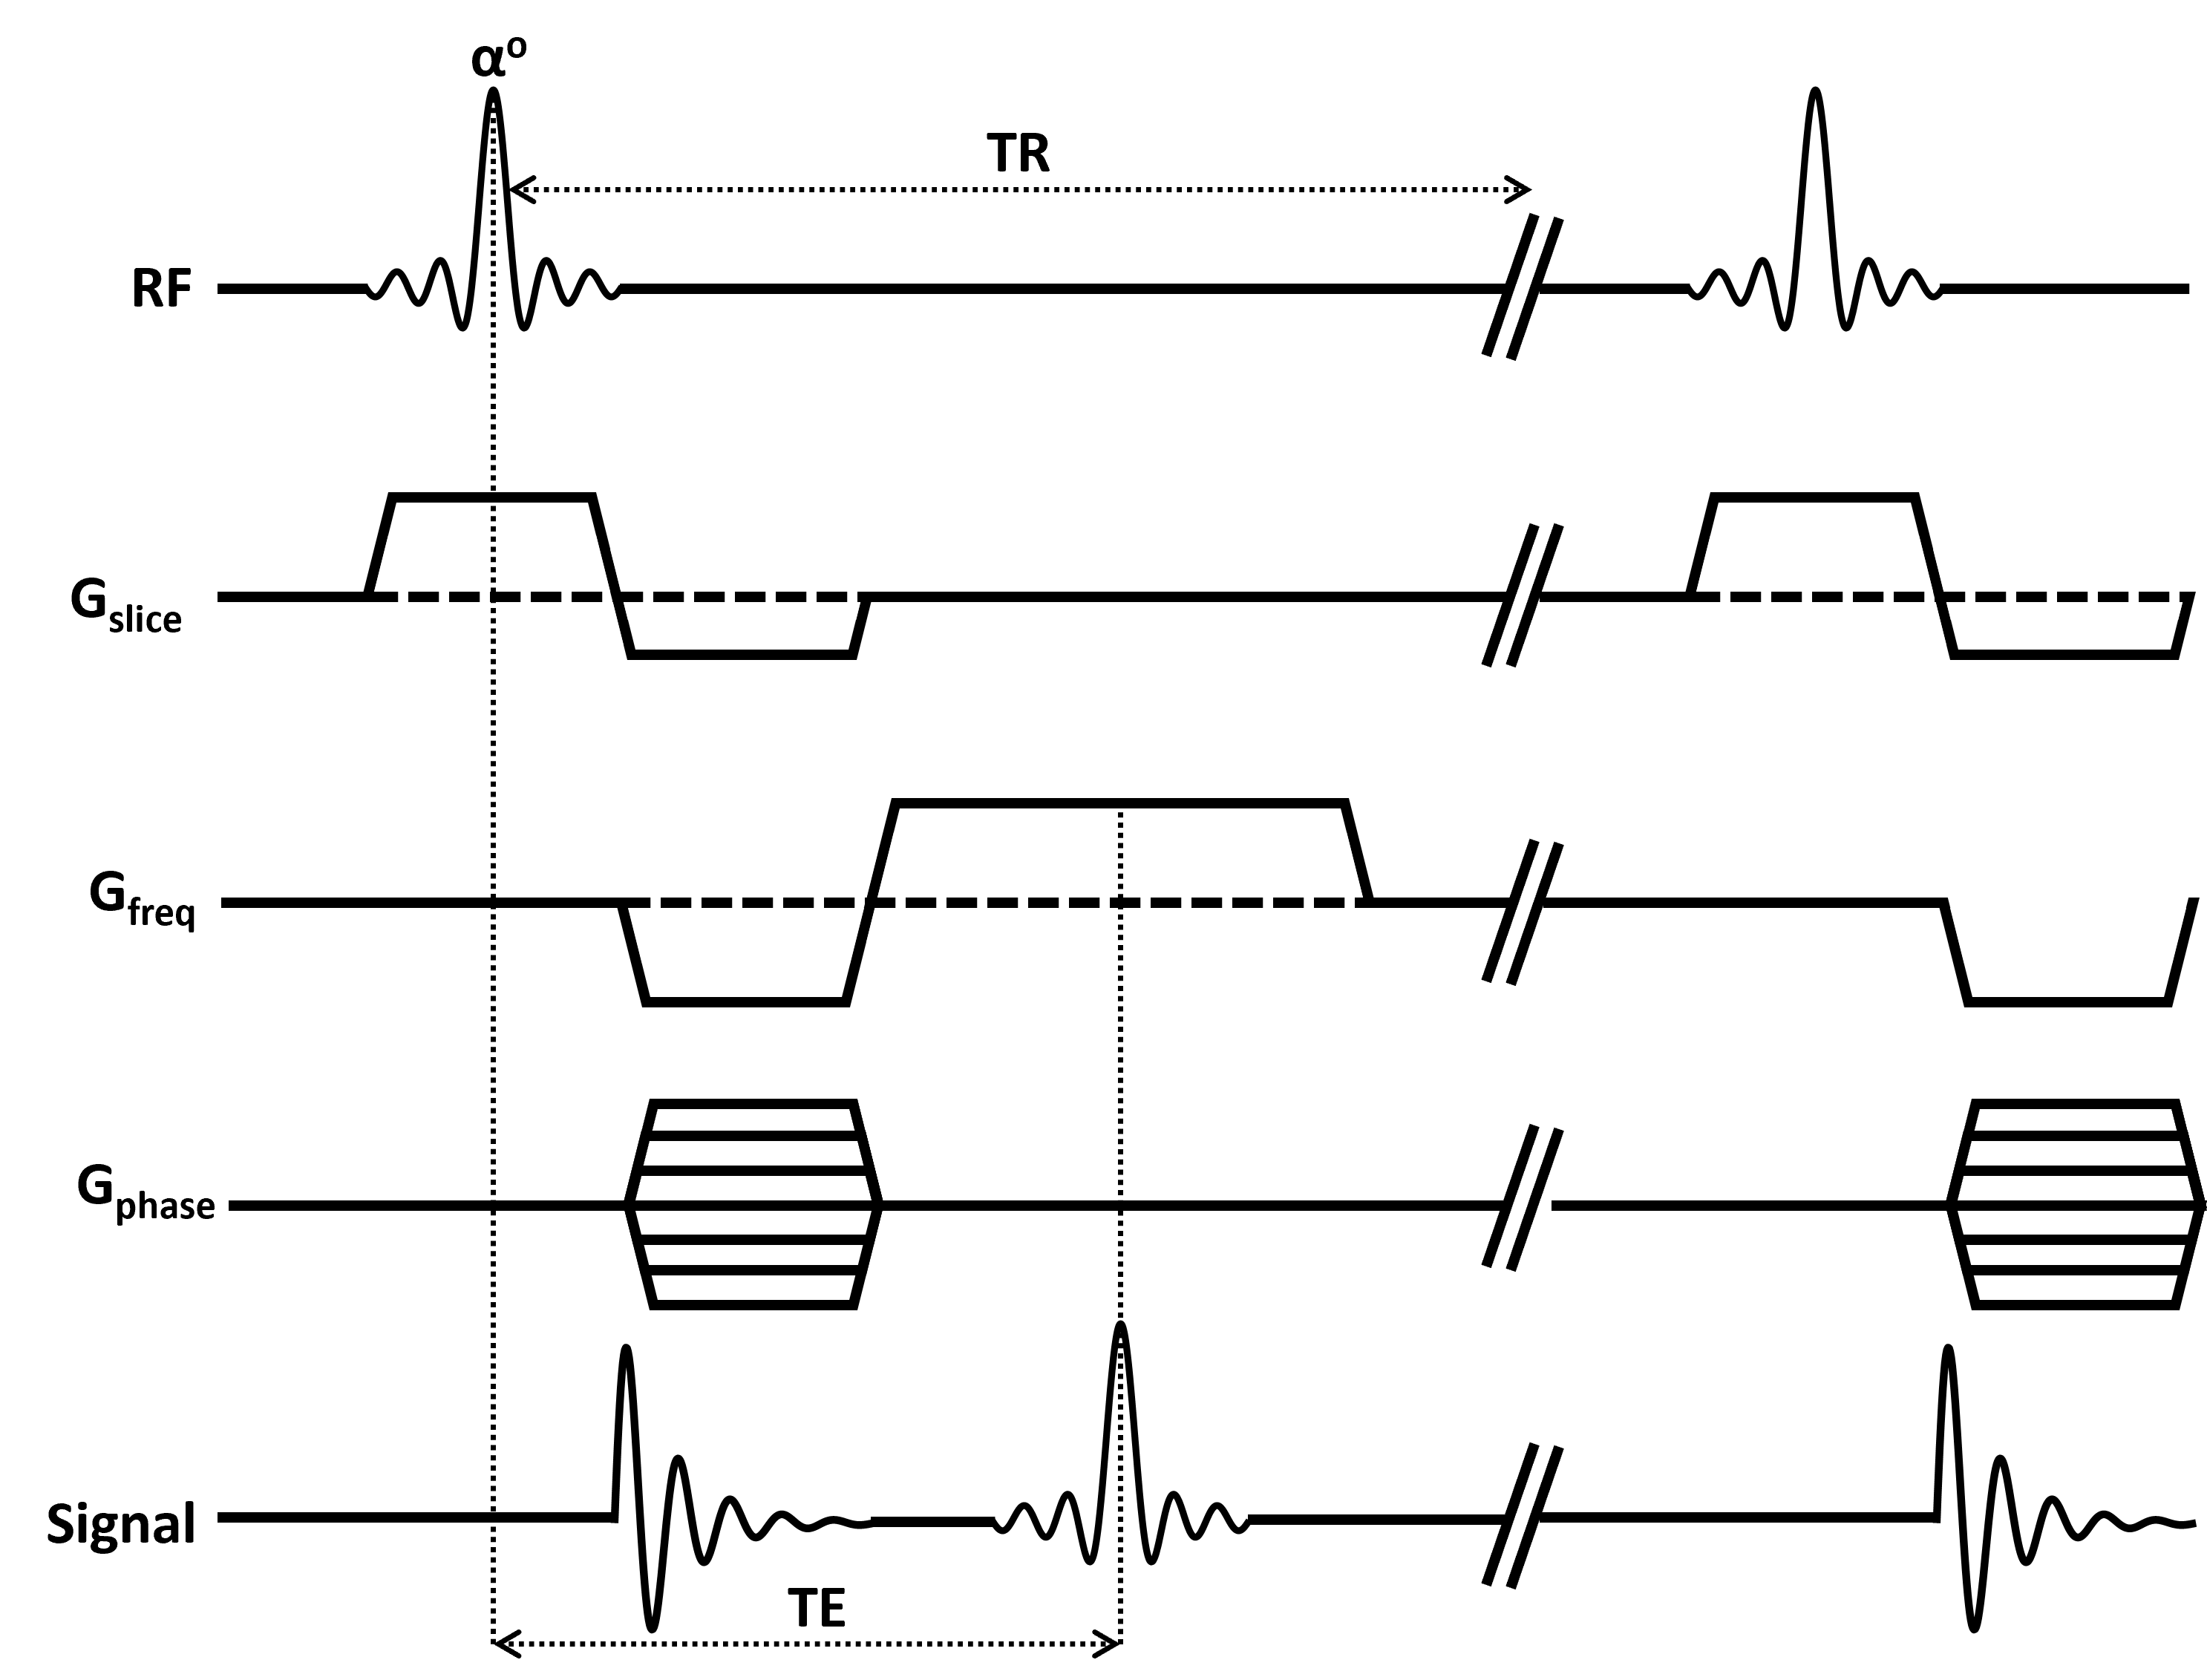
\includegraphics[width=0.9\textwidth]{Figures/Theory/GRE_sequence.png}
    \caption{\textit{Example pulse sequence diagram for a \ac{GE} imaging sequence, with the \ac{TE} indicated.}}
    \label{fig:theory:GRE}
\end{figure}

The longitudinal and transverse relaxation time constants will vary depending on the tissue. Therefore, when a particular pulse sequence is used the choice of \ac{TR} and \ac{TE} will effect the the contrast in the image. There are three main types of contrast in an image T$_1$-weighted, T$_2$-weighted and spin density weighted. The contrast in spin-density images comes from the difference in the density of spins in a particular tissue being emphasised, remembering most commonly the spin of interest is $^1$H therefore its the proton density that gives the contrast. As expected then the contrast in T$_2$-weighted images is emphasised by differences in T$_2$ times of different tissues, in order to produce these images long \ac{TR}'s and long \ac{TE}'s are used which minimises effects from different T$_1$'s. Finally in T$_1$ weighted images the contrast is dominated by differences in the T$_1$ times of different tissues, this is done by choosing short \ac{TR}'s and \ac{TE}'s which minimises effects from different T$_2$ times. T$_1$ images are often used to represent anatomical structural information as the contrast differences from these images most closely represents real-world visual differences. 

To maximise the \ac{SNR} obtained from a specific pulse sequence often depends on how quickly data can be acquired so more averages can be applied. One of the biggest aspects of scanning that affects the time taken is how data in k-space is obtained (k-space traversal). Therefore by traversing k-space more efficiently, scan time can be reduced which can make scanning more comfortable or can be used to improve \ac{SNR} by increasing averages. One of the biggest improvements in the traversing of k-space came with the development of \ac{EPI} \cite{Stehling1991Echo-planarSecond}.

\subsection{MRSI}

Acquiring MR spectra allows chemical and molecular concentrations to be obtained by comparing peaks/signals at different chemical shifts. Whilst MR images provides good contrast for structural differences. It is possible to acquire information on both chemical/molecular concentrations as well as structural information using a technique called \ac{MRSI}, which is effectively a combination of \ac{MRS} and MRI. This technique works by acquiring spectra from small volumes that are packed together into a 2D/3D grid that covers a larger volume/tissue. The voxels are often much larger than what would usually be acquired using \ac{MRI}, but are much smaller than what would be acquired using \ac{MRS} strategies. By calculating concentrations for the visible molecules in each spectra the spatial distribution of each molecule can therefore be represented as a coarse image, this is often overlayed onto an anatomical images so that the corresponding regions can be easily identifiable. Concentration changes in specific tissues can therefore be used as bio-markers for disease. In order to obtain this type of data different pulse sequences are used that use different orientations of \ac{RF} pulses and gradients. 

\subsubsection{Chemical Shift Imaging}

The simplest and quickest method to acquire 1D \ac{FID}/spectral data is to apply an \ac{RF} pulse in a static magnetic field and acquire data immediately after the pulse. It has then been shown that applying a gradient during the excitation is used to localise the data from a specific slice in the body. Usually this gradient is applied in the z-direction to localise the signal from a transverse slice through the body, however any direction of gradient can be used to excite a region. For example a sagittal or a coronal slice can be excited instead. The combination of these gradients increases the number of dimensions where data can be acquired, as has been shown with gradient echo imaging in Figure \ref{fig:theory:GRE}. Therefore, by applying gradients in all three cartesian directions simultaneously only data from a small voxel is excited, if data is acquired during the full length of an \ac{FID}that will only come from one small voxel. By iteratively changing the strengths of the adjacent voxels are excited eventually a full 2D/3D grid of spectra is obtained, this pulse sequence is called \ac{CSI}. A diagram of the pulse sequence used to acquire a 2D \ac{CSI} is shown in Figure \ref{fig:theory:CSI}.

\begin{figure}[h]
    \centering
    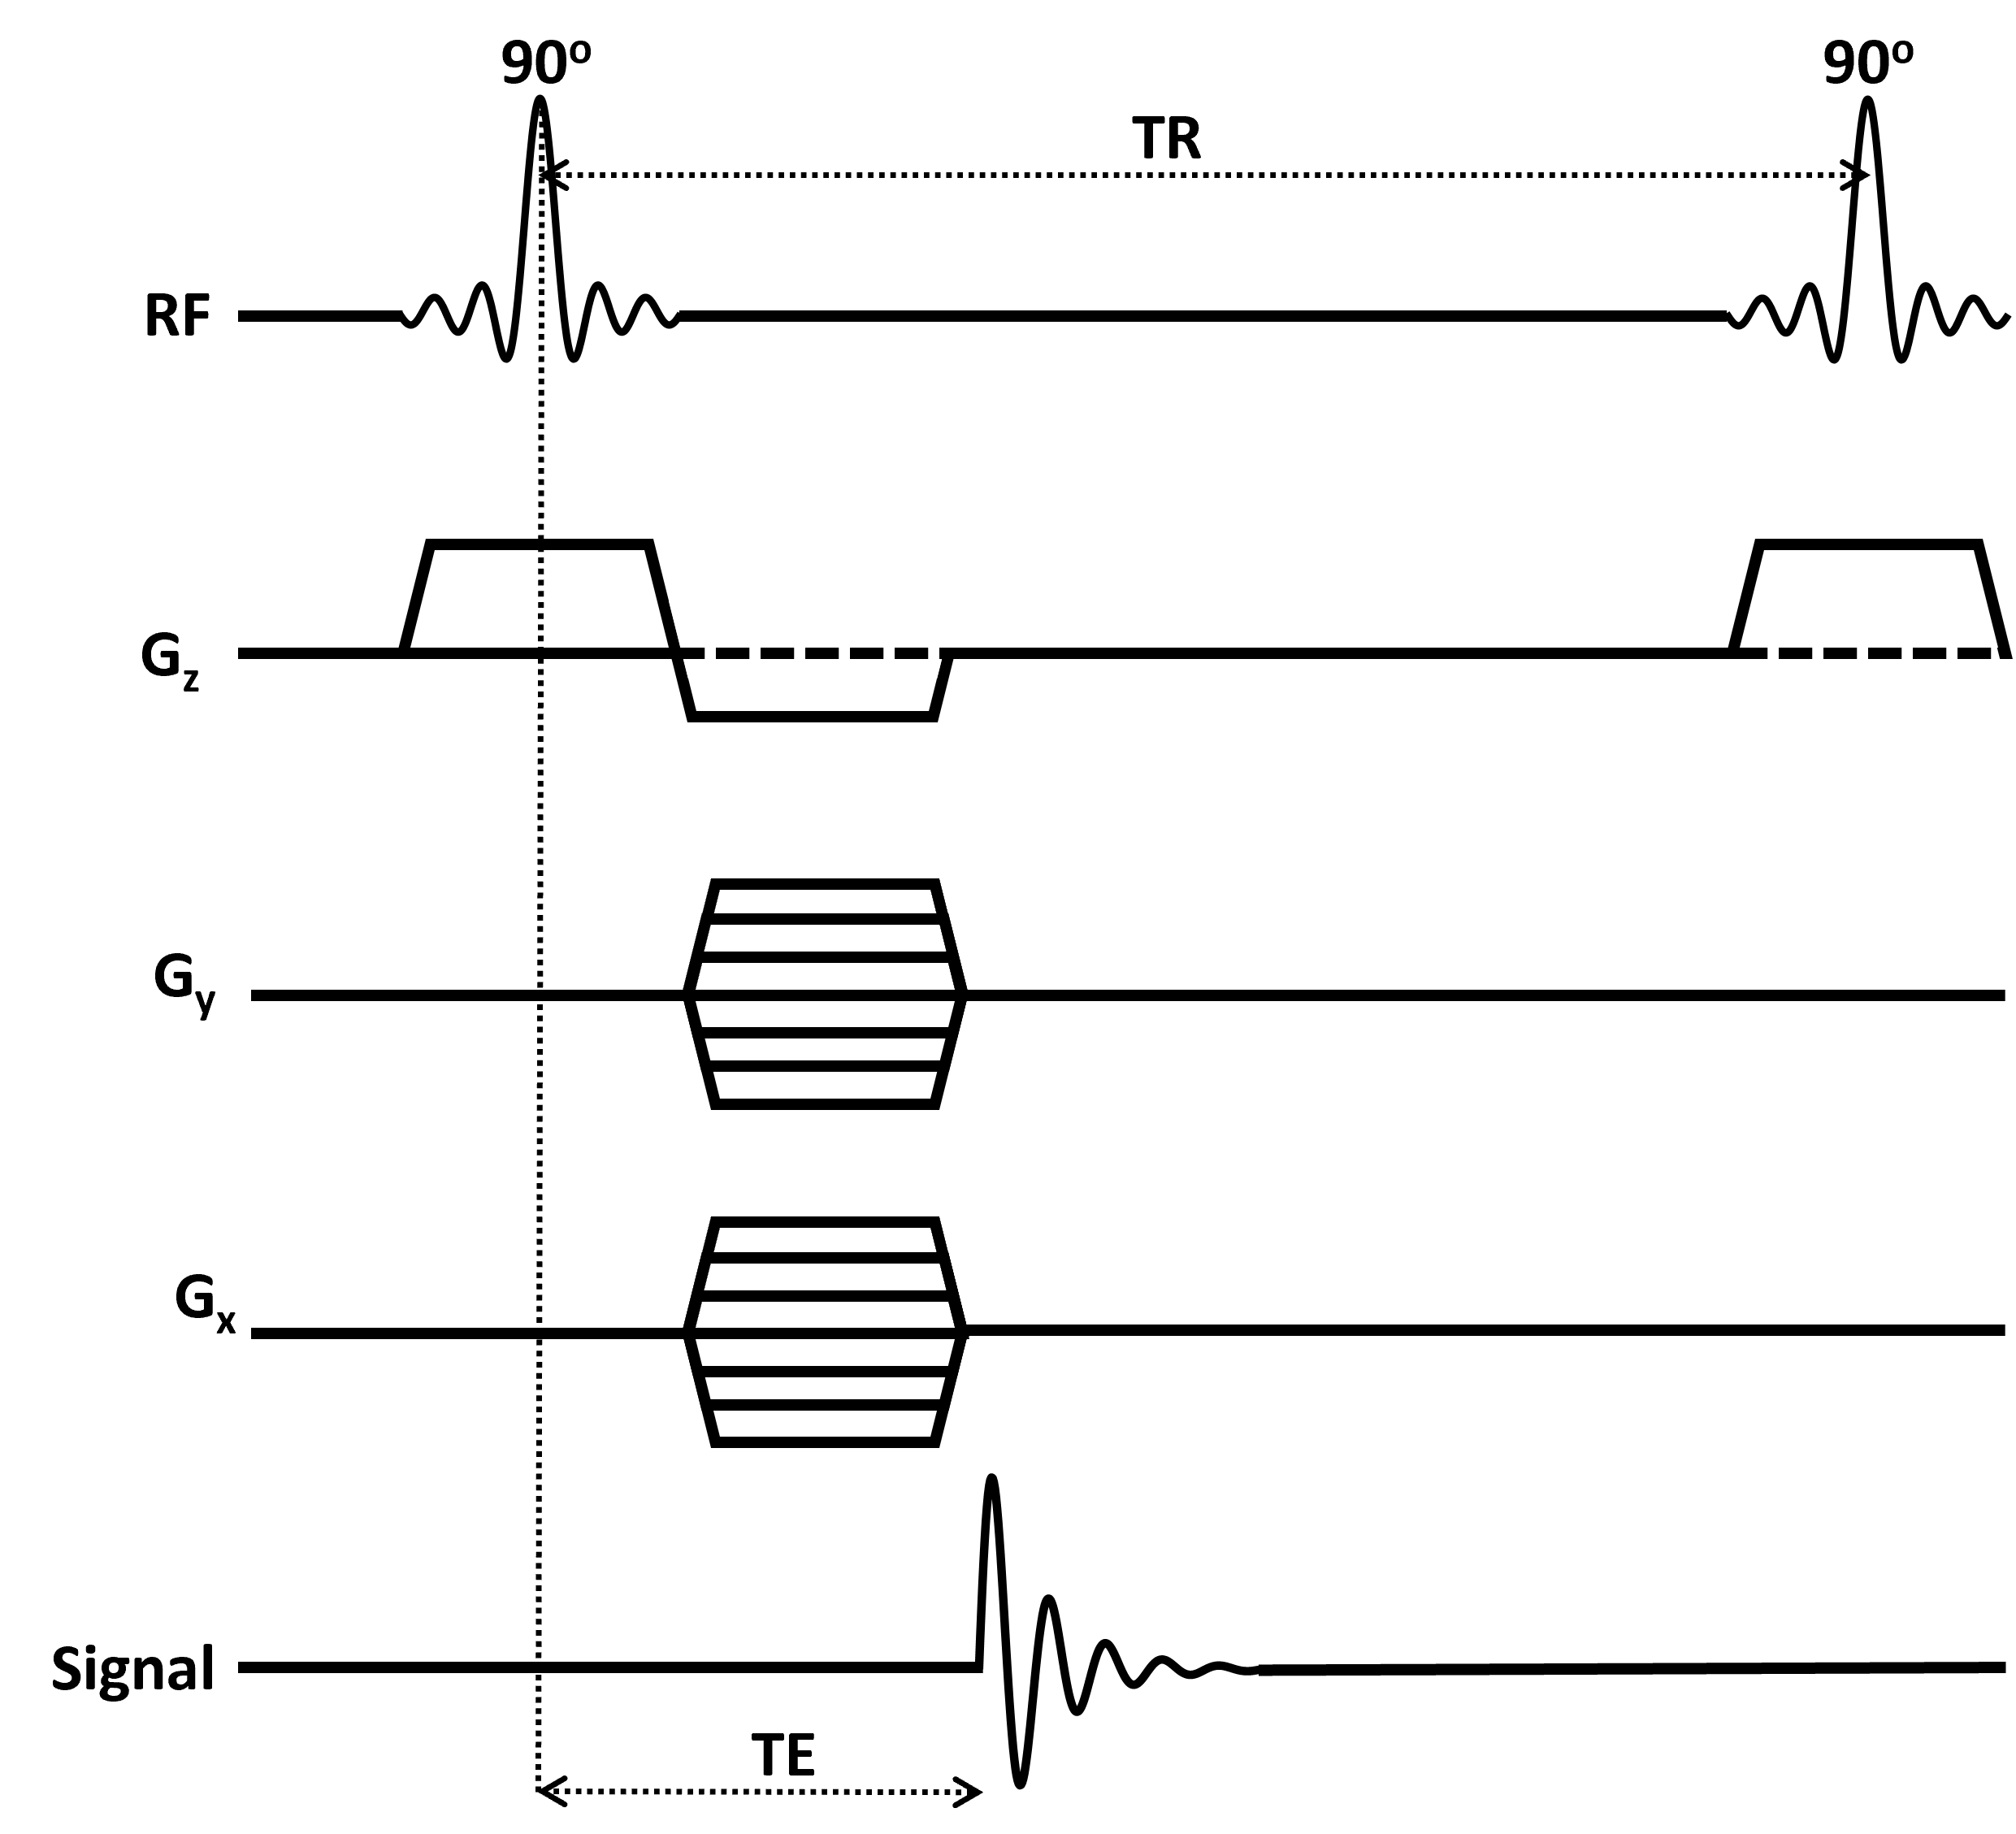
\includegraphics[width=0.9\textwidth]{Figures/Theory/CSI_sequence.png}
    \caption{\textit{Example pulse sequence diagram for a 2D \ac{CSI}.}}
    \label{fig:theory:CSI}
\end{figure}

\ac{CSI} has been used for different nuclei ($^{13}$C, $^{31}$P and $^2$H) to create maps that show the distribution of different metabolites. Acquiring this type of data which can be a problem is functional data was to be acquired, which motivates work to decrease the acquisition time for \ac{MRSI} data.

\subsubsection{EPSI and SSFP}

One of the first developments into decreasing imaging time was the introduction of \ac{EPI}. In usual \ac{GE} imaging the position in k-space returns back to zero, \ac{EPI} takes advantage of the position in k-space after an echo instead of letting it return to zero. By using multiple echoes and the use of small gradients to slightly change the position in k-space an entire 2D image can be obtained. Therefore \ac{EPI} refers to the use of a single \ac{RF} excitation to obtain an entire 2D k-space data-set. This has been implemented in imaging since 1977 \cite{Mansfield1977Multi-planarEchoes}. This technique can also be applied to \ac{MRSI} to reduce scan time, this comes in the form of a relatively new pulse sequence called \ac{EPSI} \cite{Mulkern2001EchoImaging}. Unfortunately in \ac{MRI} there are very few situations where a positive benefit comes without associated negatives. This is no different with \ac{EPSI} as there is a reduction in \ac{SNR} that is equivalent to the reduction in scan time. The most common way to recover this \ac{SNR} is to increase the number of averages of the scan, however in order to recover all of the \ac{SNR} the averages needed would make a typical \ac{EPSI} and \ac{CSI} scan take the same amount of time \cite{Mulkern2001EchoImaging}. This may at first seem like a wasted exercise, however in some fields the reduction in \ac{SNR} maybe worth the trade-off as it makes \ac{MRSI} much more clinically viable. Also, since the \ac{EPSI} sequence has much more components than \ac{CSI} such as the gradients and echoes, there is more opportunity for development which can then improve \ac{SNR}, spectral resolution and/or scanning time even further. It has been shown that the use of multiple echoes can increase the spatial resolution without adding extra scan time \cite{Furuyama2011Multi-echo-basedScanner}. This has also been shown (along with an increased temporal resolution) by using acquisition in a single excitation and using parallel imaging (also called \ac{SENSE}) \cite{Posse2009Single-shotImaging}. Because of this and the useful trade-off between scan time and SNR, \ac{EPSI} has been successfully implemented in \ac{HP} metabolic imaging \cite{Topping2020AcquisitionNuclei,Eldirdiri2018DevelopmentScanner} and using $^2$H in the liver \cite{Min2023Deuterium7T}.

\begin{figure}
    \centering
    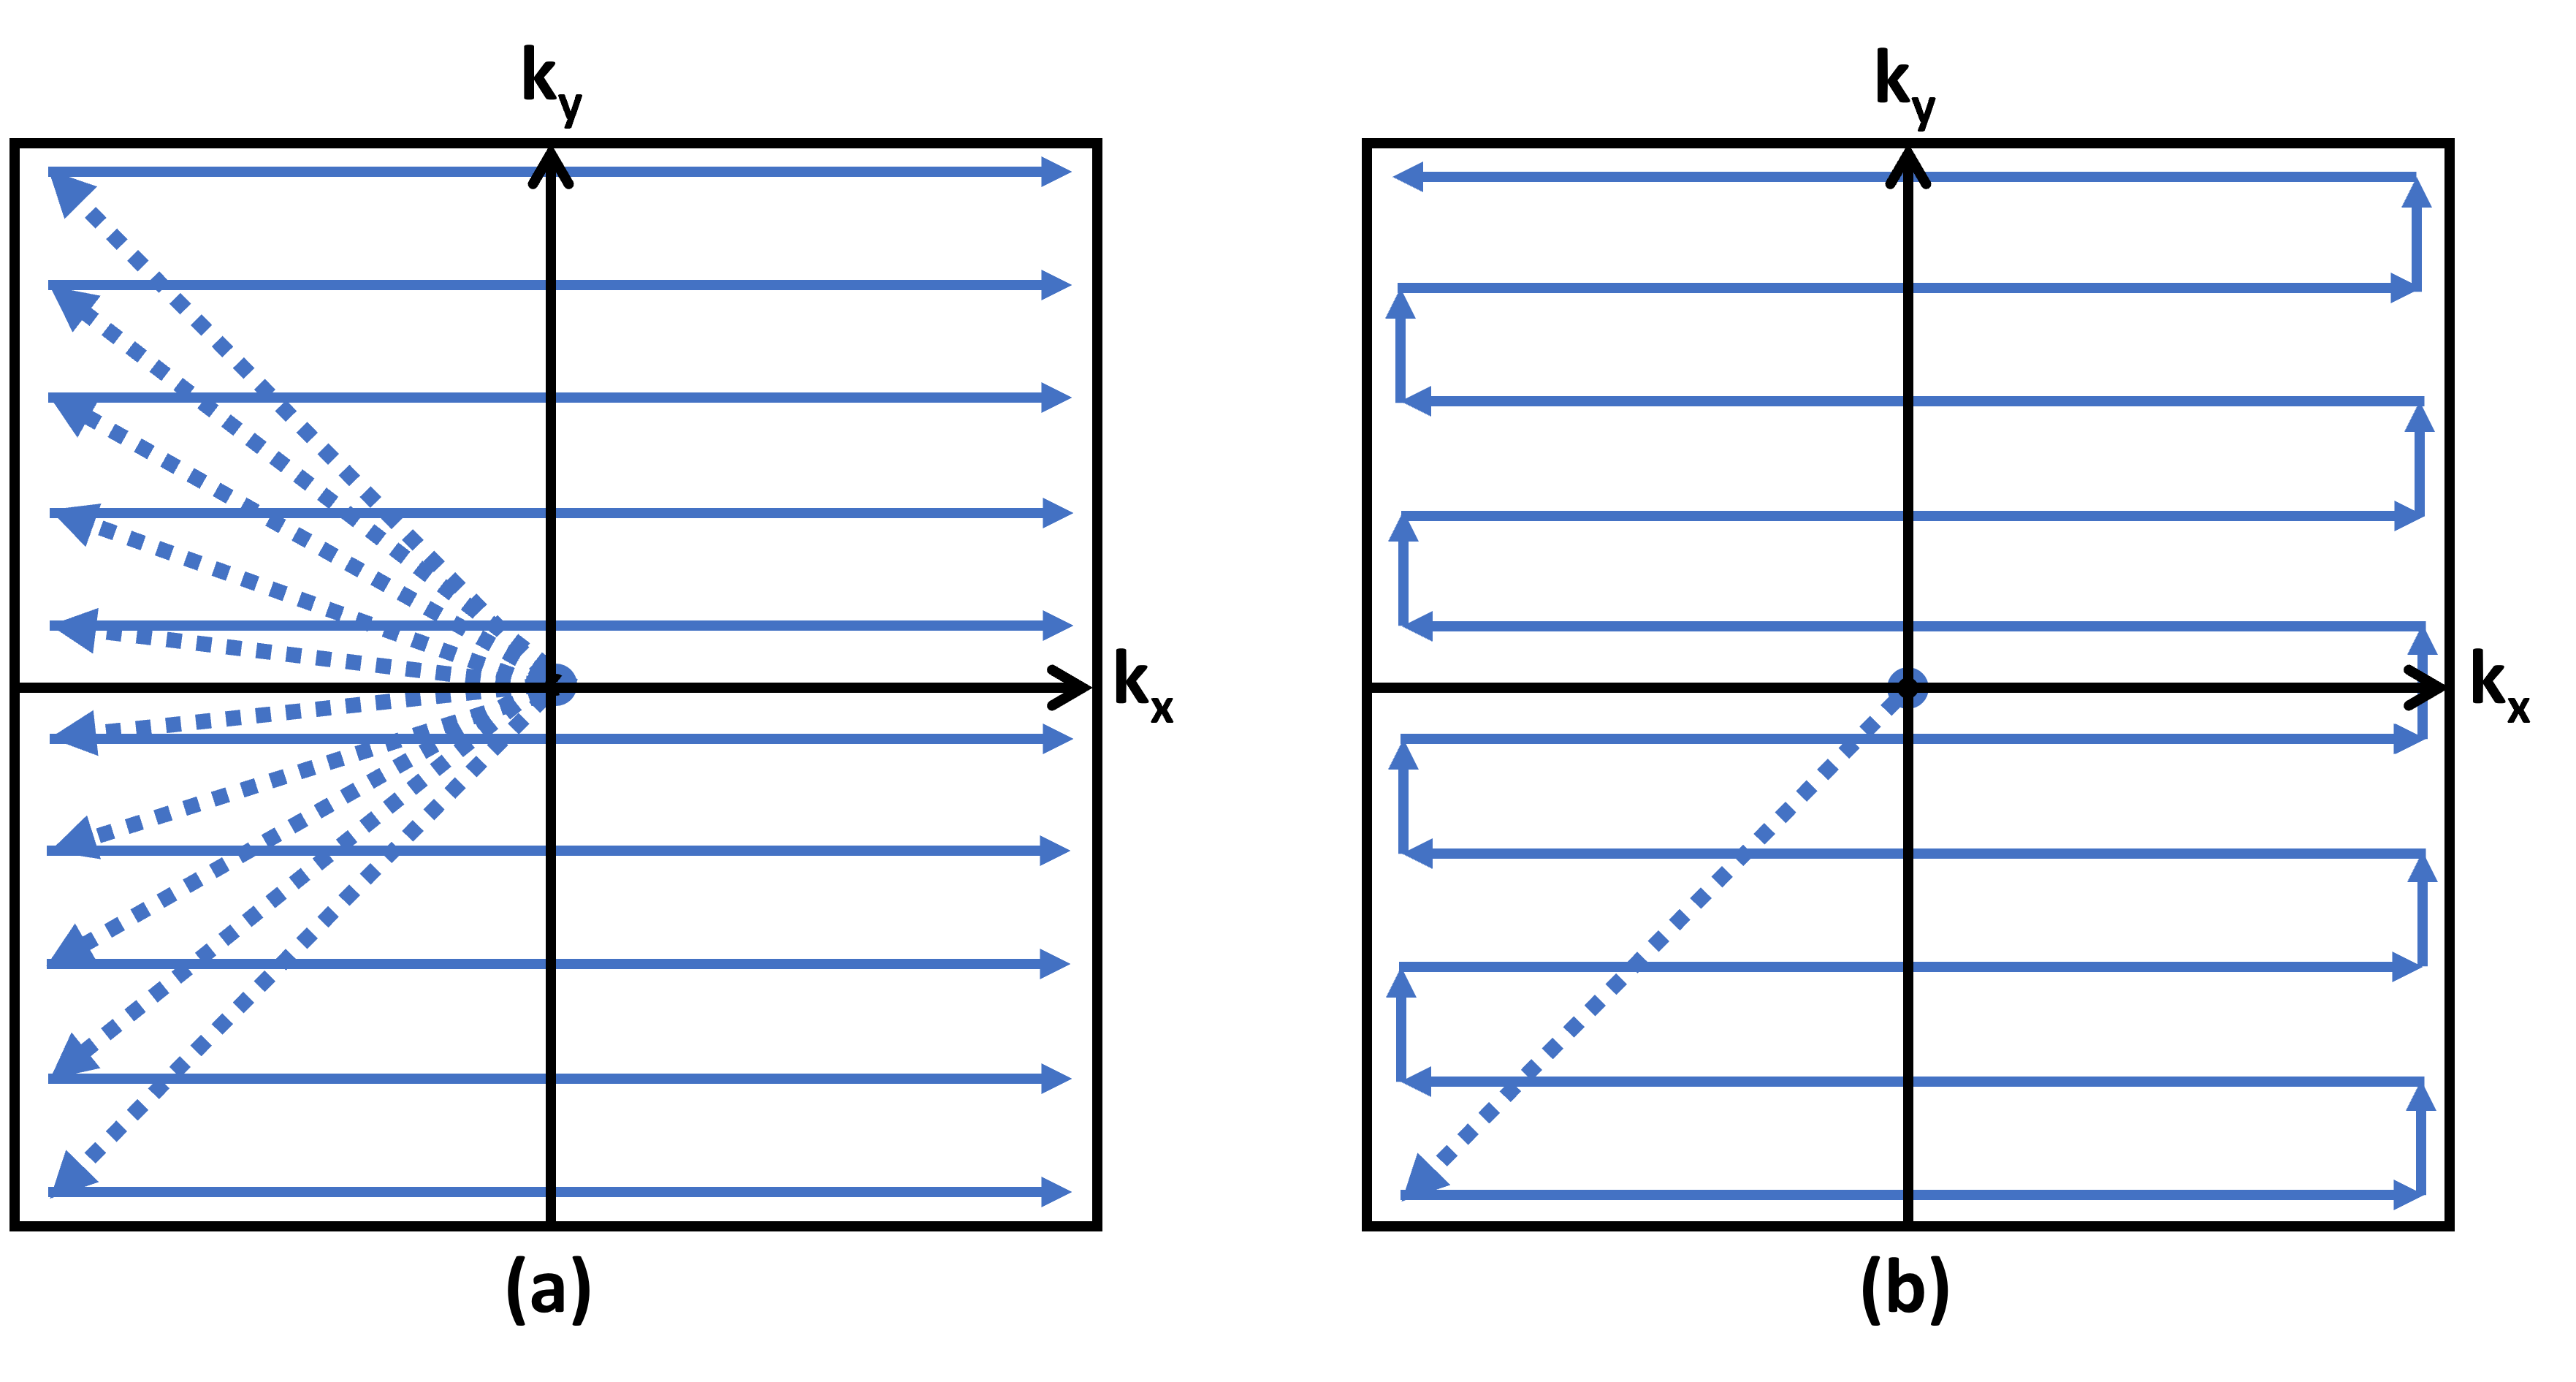
\includegraphics[width=0.9\textwidth]{Figures/Theory/kspace.png}
    \caption{\textit{2D k-space traversal paths for a gradient-echo acquisition (a) and a echo-planar image acquisition.}}
    \label{fig:theory:kspace}
\end{figure}

Balanced \ac{SSFP} \cite{Carr1954EffectsExperiments} is a special form of \ac{SSFP} where additional gradients are used to reduce off-resonance effects. \ac{SSFP} already known to increase \ac{SNR} compared to \ac{GE} imaging  \cite{Bieri2013FundamentalsMRI}, for situations where the T$_1$ to T$_2$ ratio is high (as \ac{SSFP} images have T$_1$/T$_2$ contrast). By using \ac{ME} \ac{SSFP}, with varying echo-times, it is possible to achieve good spectral separation of signals from the different metabolites, as the phase evolution between the metabolites across echoes will be different. So by combining the images for each echo as a non-linear problem using the IDEAL framework \cite{Reeder2007Water-fatImaging} metabolite maps, that appear similar to those acquired using \ac{CSI}, can be acquired. In doing this the \ac{SNR} enhancement of \ac{SSFP} is still maintained \cite{Peters2021ImprovingInvestigation}. The problem in doing this is the \ac{SNR} of this method will be higher for larger field strengths as the long echo-train needed to achieve phase separation of the different metabolite signals means that \ac{TR} is now too long to achieve sufficient \ac{SNR} gain (\ac{TR} $<<$ T$_1$ and T$_2$), this means the possible \ac{SNR} gain at lower field strengths needs to be explored. This has also only been performed for three different metabolites whereas this realistically needs to be able to analyse more metabolites which becomes much more complex. An alternative way of acquiring/analysing \ac{SSFP} data with spectrally separate metabolites is to alter the phase steps between successive \ac{RF} pulses in scans instead of the echo time, as it is much easier to separate multiple resonances and still keeps the \ac{SNR} increases of \ac{SSFP} which has been done using $^{13}$C \cite{Varma2016SelectiveSSFP}.

\section{Analysis}

\subsection{Quantification of MRS data}

When analysing \ac{MRS} data it is important to be able to accurately track changes for each spectra. The oldest method of doing this is peak integration whereby the spectra points are summed together, each MR signal will technically have an infinite width so summing over a wide enough range is important. An integration range of at least two \ac{FWHM}'s is enough to get accurate quantification \cite{Near2021PreprocessingRecommendations}. This value can also be obtained from the time-domain signal as the first point in the absorption spectra, as well as from the product of the \ac{FWHM}, $\pi$ and the peak-height in the frequency spectra \cite{deGraaf2019InSpectroscopy}. This technique is simple to implement computationally and takes little time, however needs correctly phased spectra as any incorrect phasing will give the incorrect amplitude. Most biological tissues and processes involve complex chemical environments with many different compounds which will produce different MR signals which will appear at different frequencies (also known as chemical shifts). Which will not necessarily effect the peak integration method as long as each peak/signal has a large enough frequency offset to each other, however this is commonly not the case especially in $^1$H spectroscopy \cite{Alger2010QuantitativeReview}. 

Therefore, a different methodology is needed to overcome this issue, which comes in fitting spectral signal to lineshapes such as Lorentzian \cite{Lorentz1895TheHeat}, Gaussian and Voigt \cite{Near2021PreprocessingRecommendations}. The fitting depends on a few main parameters which are the linewidth (similar to \ac{FWHM}), frequency position, phase and most importantly amplitude. By iteratively changing these parameters it is possible to minimise the difference between the fitted and the experimental signal \cite{Vanhamme2001MRMethods}, it is possible to optimise the fitting parameters and therefore the accuracy of the overall fitted signal. This method is none as a non-linear least squares \cite{Golub1973TheSeparate} fitting and is the backbone of many modern day \ac{MRS} analysis packages. This is not performed on a peak-by-peak basis, a full spectra comprising of many MR spectra is fit to the experimental data whereby the signal from each expected signal is summed together. Therefore, the more signals present in the spectra the more difficult computationally this becomes, therefore there is a strong motivation to reduce the number of parameters, reduce the computational load and therefore increase the reliability of the fitting \cite{Near2021PreprocessingRecommendations}. It has been shown that one way to improve the reliability of fitting spectra that suffer from lots of overlapping signals, which is the case for $^{31}$P \ac{MRS} data, is to use prior knowledge \cite{Hamilton2003PriorSpectra}. Some of the overlapping signals while distinctly different can share common ratios between some of their fitted parameters, one of the first fitting algorithms to include prior knowledge was the \ac{VARPRO} method \cite{Golub1973TheSeparate} which has successfully been used to analyse $^{31}$P data \cite{vanderVeen1988AccurateKnowledge,Stubbs199631P-MagneticADP}. Whilst \ac{VARPRO} was successful a new methodology was developed called \ac{AMARES} which fits more reliably and accurately as well as having increased functionality, including lineshape choice (VARPRO restriced to Lorentzian only), fitting echo signals and imposing upper and lower bounds on fitting parameters \cite{Vanhamme1997ImprovedKnowledge}. \ac{AMARES} is used regularly in \ac{MRS} analysis and is included in software packages such as JMRUI \cite{Stefan2009QuantitationPackage} and OXSA \cite{Purvis2017OXSA:MATLAB}, which have been used to analyse $^2$H \ac{MRS} data \cite{Simoes2022GlucoseGlioblastoma,Kreis2020MeasuringMRI,Kaggie2022DeuteriumMetabolism}. 

Even \ac{AMARES} has its limits and signal fitting can struggle when many peaks are present especially in terms of overlapping signals, which is a big problem in $^1$H \ac{MRS} data. Therefore, a new methodology was developed to overcome this called linear combination and was made into a toolbox that is still used called LCModel \cite{Provencher1993EstimationSpectra}. This works by fitting total spectra for each metabolite (called basis sets) instead of individual peaks, this reduces the number of model parameters and leads to increased reliability in fitting. The basis sets can be acquired by either phantom \textit{in vitro} experiments or by numerical simulation \cite{Near2021PreprocessingRecommendations}. Because of this it is more complicated to set up so it is yet to be used commonly for the more simplified and sparse spectroscopy techniques such as $^{13}$C, $^{31}$P and $^2$H although it has been used in indirect detection of $^2$H glucose by looking at the loss in $^1$H signal \cite{Rich20201HVivo,Cember2022IntegratingHumans,Niess2023Reproducibility3T}. 

\subsection{Post-Processing Improvement of SNR}

The low \ac{SNR} of $^2$H is often a problem during scanning and as scanning times are reduced for participant/patient comfort this can be a problem in all nuclei spectroscopy. It has been common practise for a long time now to produce fitting in the time-domain compared to in the frequency domain \cite{Joliot1991InMethods}. In order to increase the reliability and reproducibility of values obtained from analysis its important to increase \ac{SNR}. A popular method of increasing the \ac{SNR} of spectra by applying spectral filtering in the form of apodisation, common lineshapes that are used in the filtering are exponential and Gaussian \cite{Goryawala2020EffectsFitting}. Applying a Gaussian filter can reduce the \ac{FWHM} of MR signals which can improve fitting reliability however this will change the lineshape of the signal, the best way to do this is to apply an exponential filter along with a Gaussian to negate the previous lineshape such that the new signal is only Gaussian. However, it has been shown that apodisation can reduce accuracy of fitting especially in cases of complex spectra where signals overlap spectrally \cite{Bartha1999FactorsFiltering}. Because of this apodisation is often used sparingly and often only used for visual demonstrations of data. Lots of alternatives exist in terms of denoising including \ac{PCA} \cite{Abdoli2016DenoisingComponents} and low rank approximation \cite{Nguyen2013DenoisingApproximations} that have shown to provide improved \ac{SNR} with damaging quantification \cite{Clarke2022UncertaintyMethods}. Low-rank denoising in the form of \ac{HOSVD} also known as Tucker-Tensor decomposition, have been used in \ac{DMI} previously \cite{Kreis2020MeasuringMRI,Assmann2020InCholesterol}. \ac{SVD} has been used previously as an alternative fitting routine \cite{Pijnappel1992SVD-basedSignals} as well as a water signal removing technique post-processing \cite{Cabanes2001OptimizationBrain}. This technique works initially on 1D spectra decomposing the spectra into a subset of vectors and singular values, the singular values represent how important each vector is in representing the data. Therefore by removing the lower singular values it is possible to remove the noise from the spectra. This can be applied to matrices in more than on-dimension where it becomes \ac{HOSVD}, the Tucker decomposition is a \ac{HOSVD} where tensors are used to factorise a matrix into a core matrix and directional tensors. The core matrix is equivalent to the singular values in \ac{SVD} and therefore reducing the core matrix removes the noise \cite{Tucker1966SomeAnalysis}. The extra dimensions in \ac{MRSI} data represent either spatial dimensions or time dimensions which will tend to be smaller than the spectral dimensions. This strategy has been implemented into a MATLAB toolbox \cite{Bader2007EfficientTensors}.

% \subsection{Concentration Calculation} % Potential
% Robins section from glucose paper 

\section{RF Coils}

\ac{RF} coils have two functions to apply a B$_1$ field to excite spins into specific energy levels or orientations, or to receive a magnetic field due to Faraday's law of induction. The profile of the applied B$_1$ field is due to the design/shape of the coil, the frequency of the applied field comes from the electronic components in the coil. The exact frequency of the B$_1$ needs to overlap with the Larmor frequency of the nuclei of interest, if the B$_1$ frequency is offset less B$_1$ field is applied to the nuclei which means the magnetisation might not be fully tipped into the transverse plane. This shows how important design and building of \ac{RF} coils are, lots of different companies exist where it is possible to buy \ac{RF} coils. This can be expensive due to the experience and time that goes into coil building, therefore it is important when starting new research with a new nuclei (such as $^2$H) to be able to build home-made coils. 

\subsection{Theory}

The simplest way to build an \ac{RF} coil is to apply an alternating current through a wire shaped into a loop (inductor) with a capacitor in parallel. This forms what is known as an RLC circuit and is often used to create a resonance for current, the voltage and current and the relationship with phase can be demonstrated through a phasor diagram which can also represent complex numbers. Therefore, many electrical components can also be represented as complex numbers. The current variation with time ($I(t)$) of an RLC circuit is shown in equation \ref{eqn:theory:Current}.

\begin{equation}
    I(t) = I_{\mathrm{max}}\sin(\omega t + \phi)
    \label{eqn:theory:Current}
\end{equation}

According to Ohm's law the voltage across a resistor ($\Delta V_R$) can be found, an inductor will oppose the current and will therefore have a corresponding reactance ($X_L$) and will be 90$^\circ$ ahead of the current. The time-varying voltage will cause the capacitor to continuously charge and discharge which resists the change in voltage and will also have a reactance ($X_C$). The voltage variations with time for each electrical component is shown below in equation \ref{eqn:theory:Voltage}. A \ac{RF} B$_1$ will flow through the coil and induce a current that will charge the capacitor, the capacitor will then dissipate energy which causes current to flow. Energy will dissipate into the resistance and therefore the current will decrease exponentially. Graphs of the change in voltage in this case are shown in Figure \ref{fig:theory:VI}, along with the corresponding absorption and dispersion curves.  

\begin{equation}
\begin{gathered}
    \Delta V_R = IR = I_{\mathrm{max}}R\sin(\omega t + \phi) \\
    \Delta V_L = \omega LI_{\mathrm{max}}\cos(\omega t + \phi) =  X_LI_{\mathrm{max}}\cos(\omega t + \phi)\\
    \Delta V_C = -\frac{I_{\mathrm{max}}}{\omega C}\cos(\omega t + \phi) = -X_C\cos(\omega t + \phi)\\
    \label{eqn:theory:Voltage}
\end{gathered}
\end{equation}

The RLC circuit will have a natural resonance frequency ($\omega_0$), therefore when the frequency of the applied current is the same as this natural frequency the circuit is considered on resonance ($\omega=\omega_0$). The total opposition of the circuits current flow is called the impedance ($Z$), which is given as $Z = R+i(X_L-X_C)$ and therefore when the impedance is minimised the circuit is on resonance \cite{deGraaf2019InSpectroscopy}. The natural resonance of the circuit is therefore given in equation \ref{eqn:theory:res}.

\begin{equation}
    \omega_0 = \frac{1}{\sqrt{LC}}
    \label{eqn:theory:res}
\end{equation}

The wires that the coil is connected to needs to be shielded from external fields in order to stop them acting as aerials. The most common cables that are used are coaxial cables, which has a characteristic impedance of 50$\Omega$. When a coil is constructed at the Larmor frequency that is required the impedance is most likely different to the impedance of the cable. The difference in impedance will cause some of the power to be reflected at the coil instead of transmitted. Therefore, the impedance of of the loaded wire needs to be changed which can be done by changing the reactance. The most common ways of doing this are by adding an inductor or a capacitor in parallel to the coil. The method of adding a capacitor will be discussed here and an example circuit can be seen in figure\ref{fig:theory:RLC}.

\begin{figure}
    \centering
    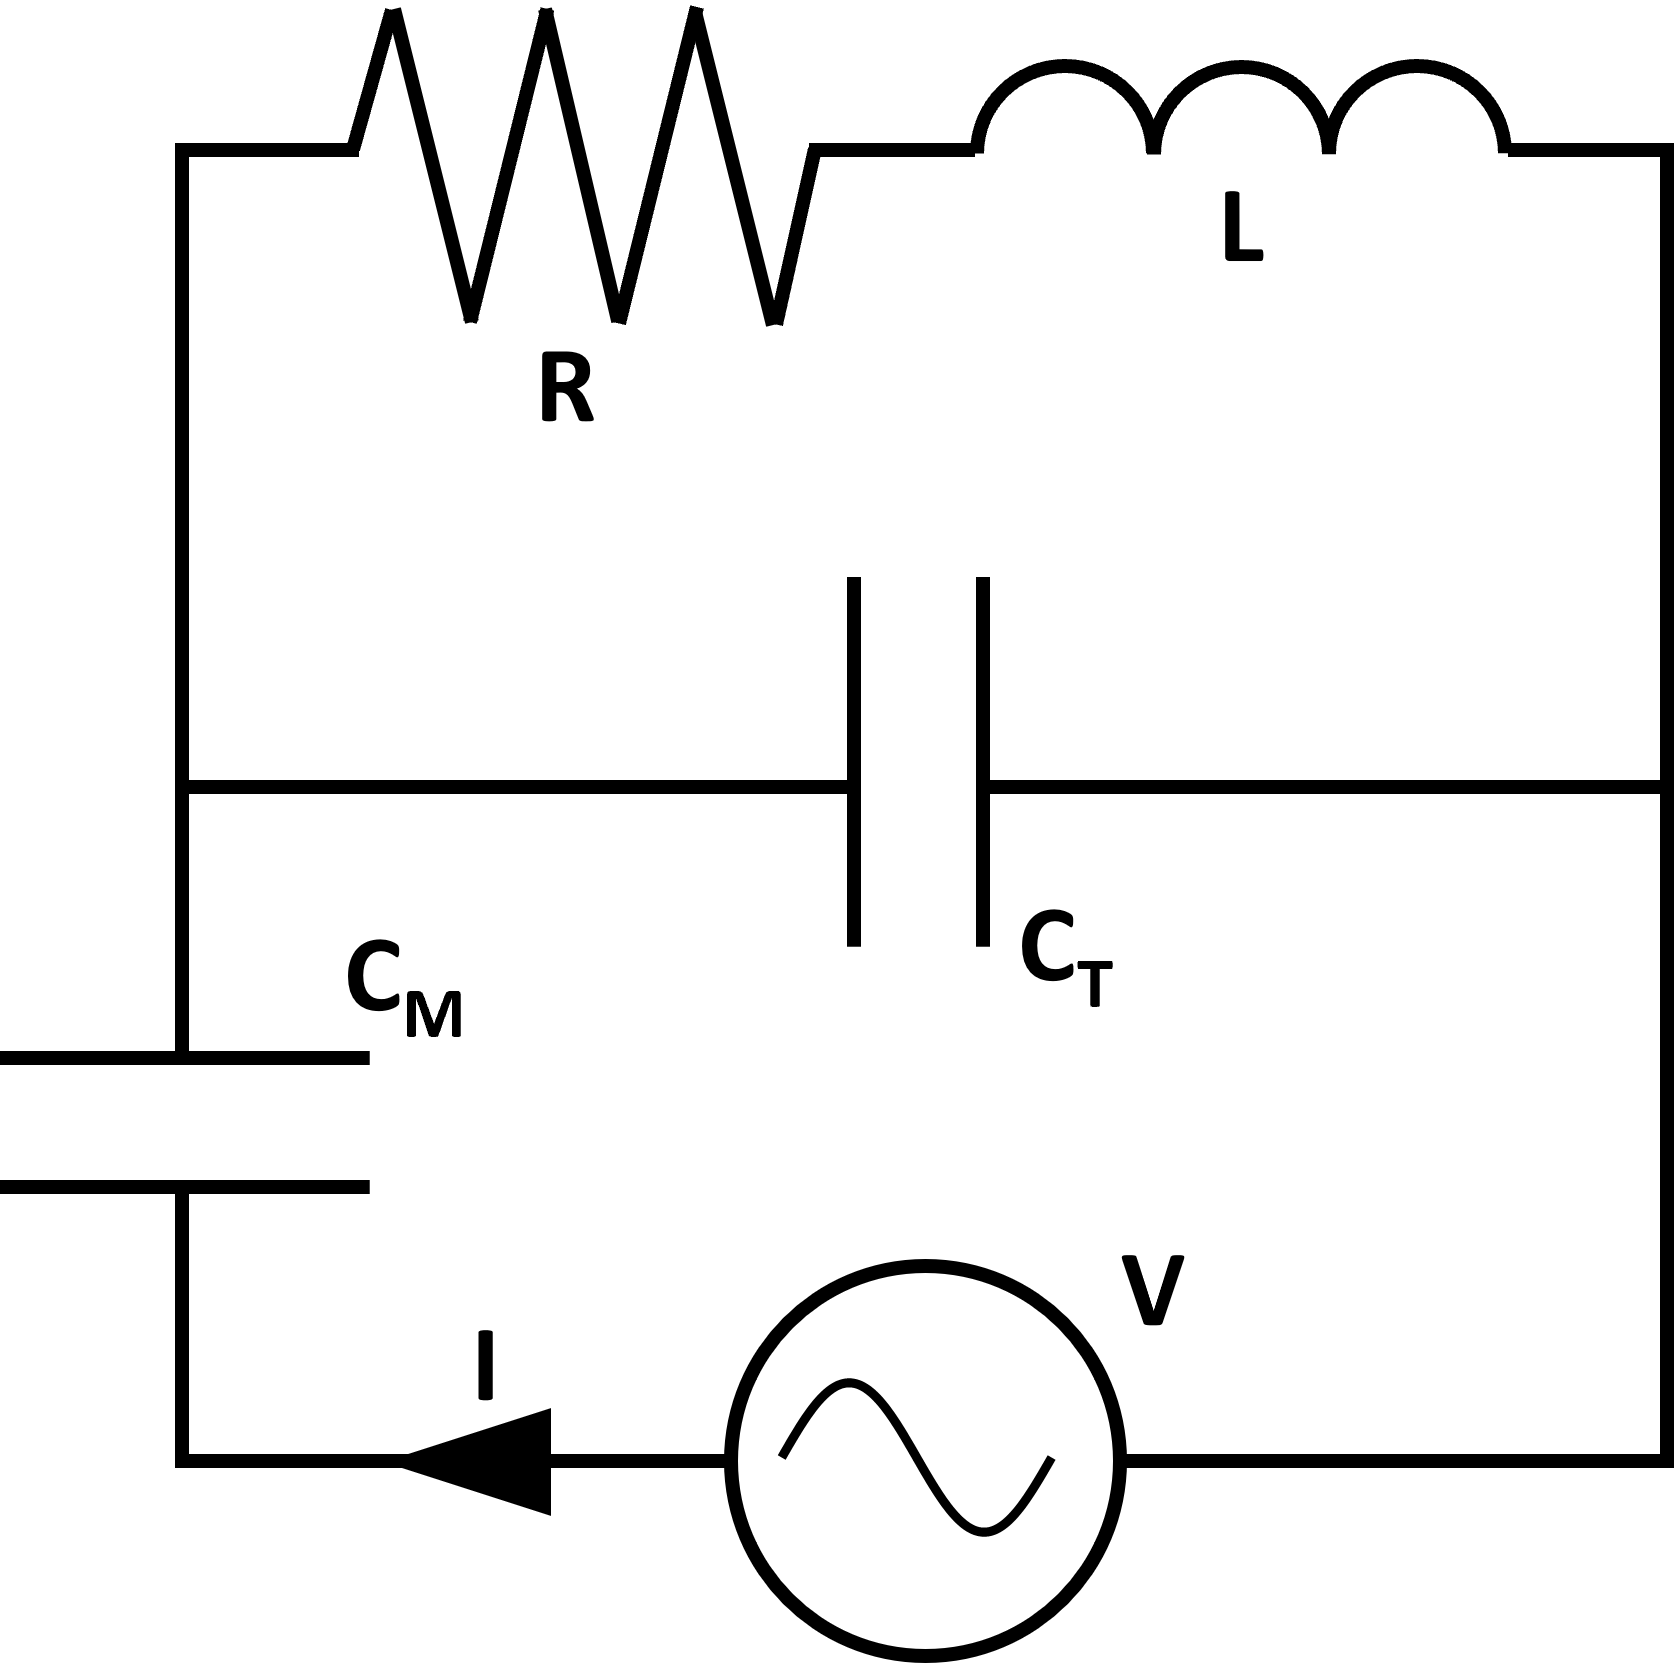
\includegraphics[width=0.6\textwidth]{Figures/Theory/RLC_Circuit.png}
    \caption{\textit{Example diagram of an RLC circuit with both tuning (C$_T$) and matching capacitor (C$_M$), along with an AC signal generator.}}
    \label{fig:theory:RLC}
\end{figure}

The capacitor in series with the coil is referred to as the tuning capacitor (C$_T$) with the other capacitor called the matching (C$_M$). The total capicitance is C$_M$+C$_T$. A relationship between C$_M$ and C$_T$ can be found that is related to the quality factor (Q) \cite{Chen1989ChapterNoise} which is the resonance frequency divided by the bandwidth of the absorption spectra in Figure \ref{fig:theory:VI}, and is shown in equation \ref{eqn:theory:match}. 

\begin{equation}
    C_M = \sqrt{\frac{C_T}{Q\omega_0Z}}
    \label{eqn:theory:match}
\end{equation}

The combination of equations \ref{eqn:theory:res} and \ref{eqn:theory:match} can be used to find the capacitance's needed to tune and match the coil \cite{Chen1989ChapterNoise}. To check a fully constructed coil an \ac{AC} is applied to the coil and the reflected power is graphed against frequency as a logarithmic scale measured in decibels (dB), the graph will appear similar to the absorption spectra in Figure \ref{fig:theory:VI}. A level of 20 dB is commonly perceived as a good enough of reflected power, with the peak appearing at the Larmor frequency. Realistically soldering and adding components will change the circuit and the theoretical components can be wrong so will often need changing based on the measured response.

\begin{figure}
    \centering
    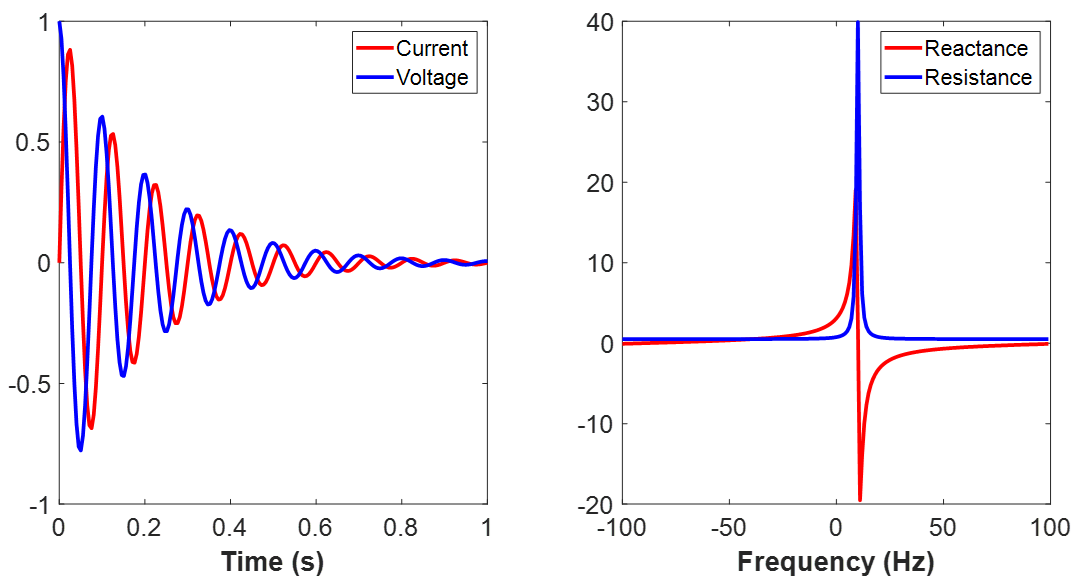
\includegraphics[width=0.9\textwidth]{Figures/Theory/VI.png}
    \caption{\textit{(a) Current and Voltage graphs for a dissipating capacitor in an RLC circuit. (b) corresponding absorption and dispersion spectra that show resistance and reactance respectively.}}
    \label{fig:theory:VI}
\end{figure}

When a coil is placed over a sample or body tissue mutual inductance takes place which changes the total inductance. This changes the overall inductance of the circuit and will therefore change the matching condition as well as the resonant frequency of the coil. Therefore it is important to load the coil with a phantom that matches the response that will be used during scanning, when designing/building the coil. 

\subsection{Coils Built}

During these works three different coil types were constructed and implemented for use on a Philips 3T Achieva system. Two surface coils, a saddle coil and a Helmholtz coil. All the coils were tuned to a single resonance of 19.6 MHz, the Larmor frequency of $^2$H at 3T. These coils were single tuned as dual-tuned coils have less power and are less efficient than single-tuned coils. A 2 L salt-water solution is used to load each coil, with varying amounts of salt. A birdcage coil dual tuned to the Larmor frequencies of $^1$H and $^2$H at 7T was purchased from Rapid Biomedical for use on a 7T Philips Achieva System. The in-house built coils were used to acquire spectroscopic $^2$H data with anatomical $^1$ images being acquired using the large built-in magnet bore as an \ac{RF} coil. The purchased coil is able to acquire $^1$H anatomical images as well as $^2$H spectroscopic data, low resolution $^2$H images were also acquired using this coil.

\subsubsection{Surface Coil}
\label{Chap:Theory:Coils}

A surface coil is the simplest and most basic coil to design and build is the surface coil, where wire forms a circular loop. The magnetic field is maximum directly in the centre of the coil and exponentially decreases, with distance from the coil. Therefore the field is spatially in-homogeneous which is why this coil design is often used for non-localised spectroscopy, where the localisation of the signal is down to the placement of the coil. The penetration depth of the magnetic field for a surface coil is approximately equal to the radius of the coil, and therefore is sensitive to regions closest to the coil. Surface coils can also be used to image unusually shaped regions of the body or sections of the body that.

\begin{figure}
    \centering
    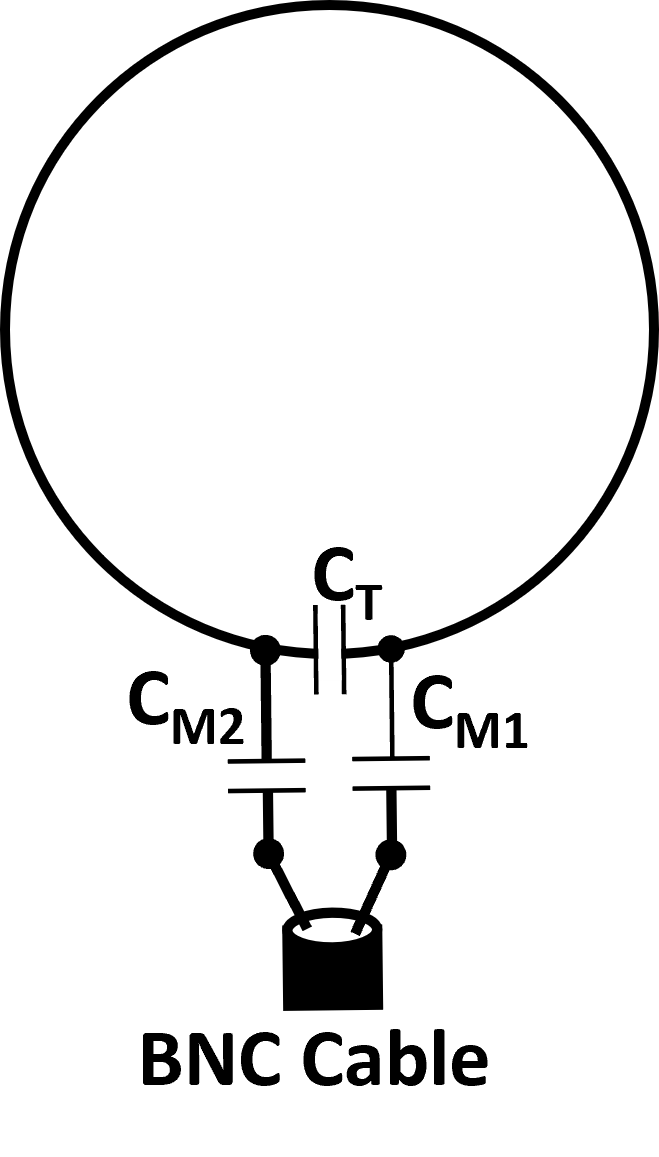
\includegraphics[width=0.3\textwidth]{Figures/Theory/Surface_Coil.png}
    \caption{\textit{Diagram of a typical planar surface coil with circuit elements attached, the coaxial cable attaches to a BNC connector.}}
    \label{fig:theory:Surface}
\end{figure}

Surface coils were originally built to practise the process of coil building, getting used to and testing the effect different capacitance values have on the reflection curve. The surface coils used for data collection were built for use in Chapter \ref{Chap:Lipid}. The first coil is a small 5 cm coil with two loops of copper wire (to keep it as circular as possible) with tuning capacitance of 173.4 pF and matching 11 pF which is split over both wires of the loop to keep it balanced. The coil is small to maximise the sensitivity to signal from subcutaneous fat in the skin.

\begin{figure}
    \centering
    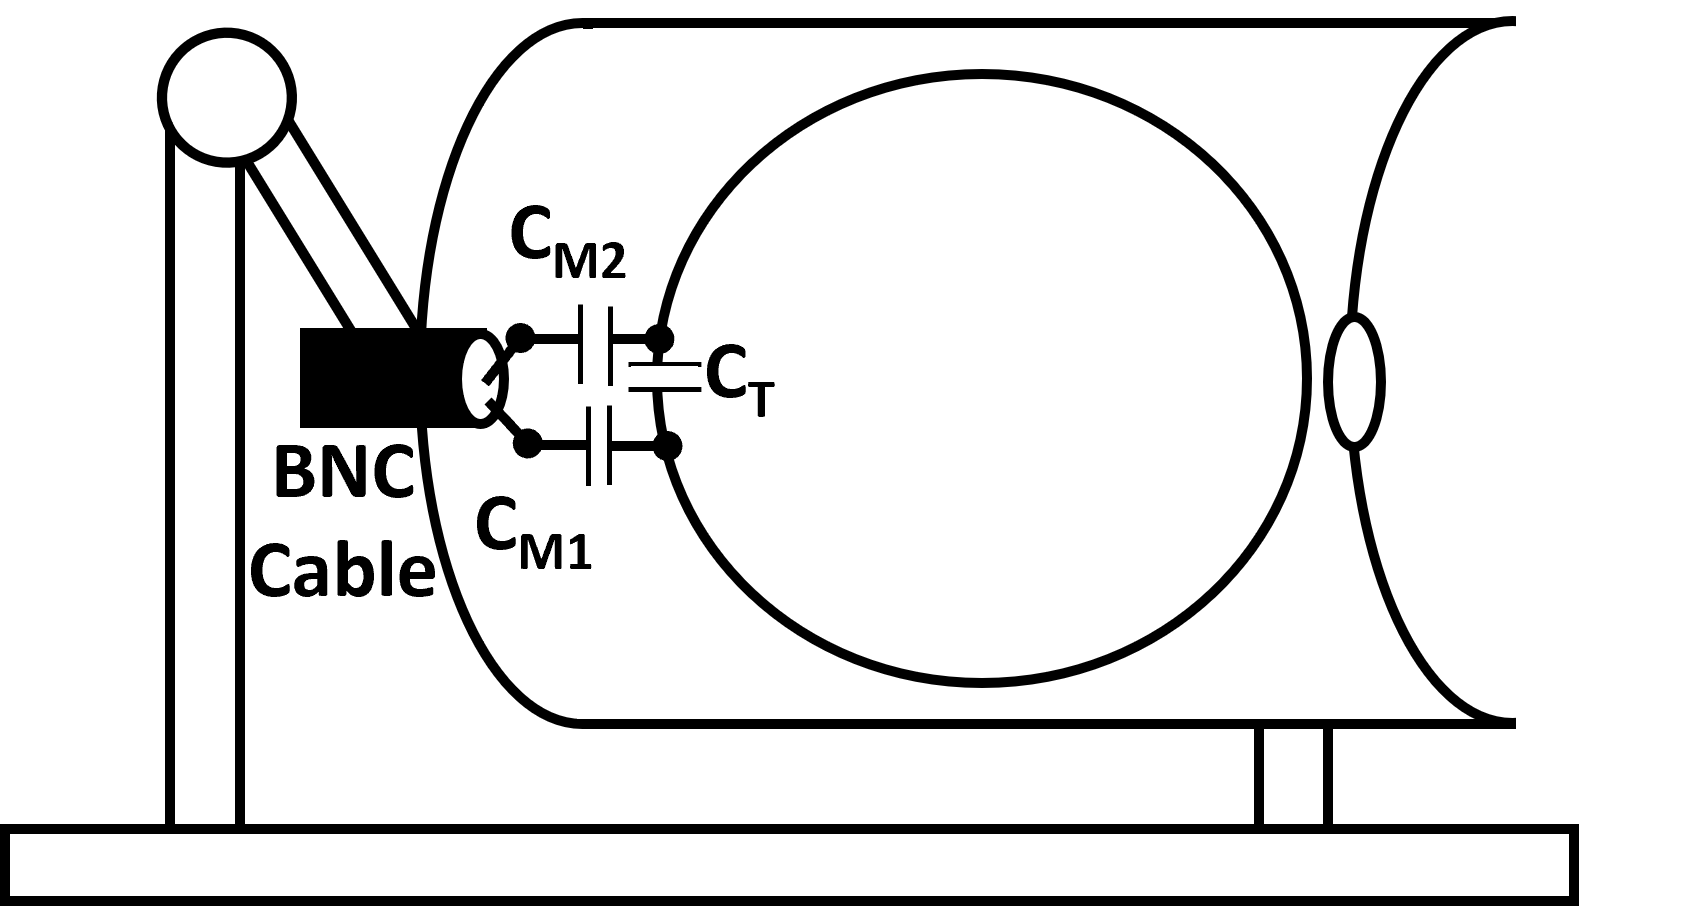
\includegraphics[width=0.7\textwidth]{Figures/Theory/Liver_Coil.png}
    \caption{\textit{Diagram of the surface coil attached to movable housing for scanning of the liver.}}
    \label{fig:theory:Liver}
\end{figure}

The second coil is 12 cm in diameter again made out of copper wire, and is designed for imaging in the liver. This coil is larger so that the penetration dept is large enough to reach the liver. The coil is slightly curved in plane in order for the coil to sit closer to the liver and is mounted to holder so that the coil can be rotated whilst still being attached to the scanner bed.

\begin{figure}
    \centering
    \includegraphics[width=0.9\textwidth]{Figures/Theory/Coil_Pics.png}
    \caption{\textit{Photos of the calf surface coil from two different angles (a \& b) with a photo of the liver surface coil (c), both tuned to the $^2$H Larmor frequency at 3T. The yellow tablets that can be seen in all the photos are vitamin tablets (also known as fiducial markers) used to identify where the coil is in an image.}}
    \label{fig:theory:Pics}
\end{figure}

\subsubsection{Saddle}

\begin{figure}
    \centering
    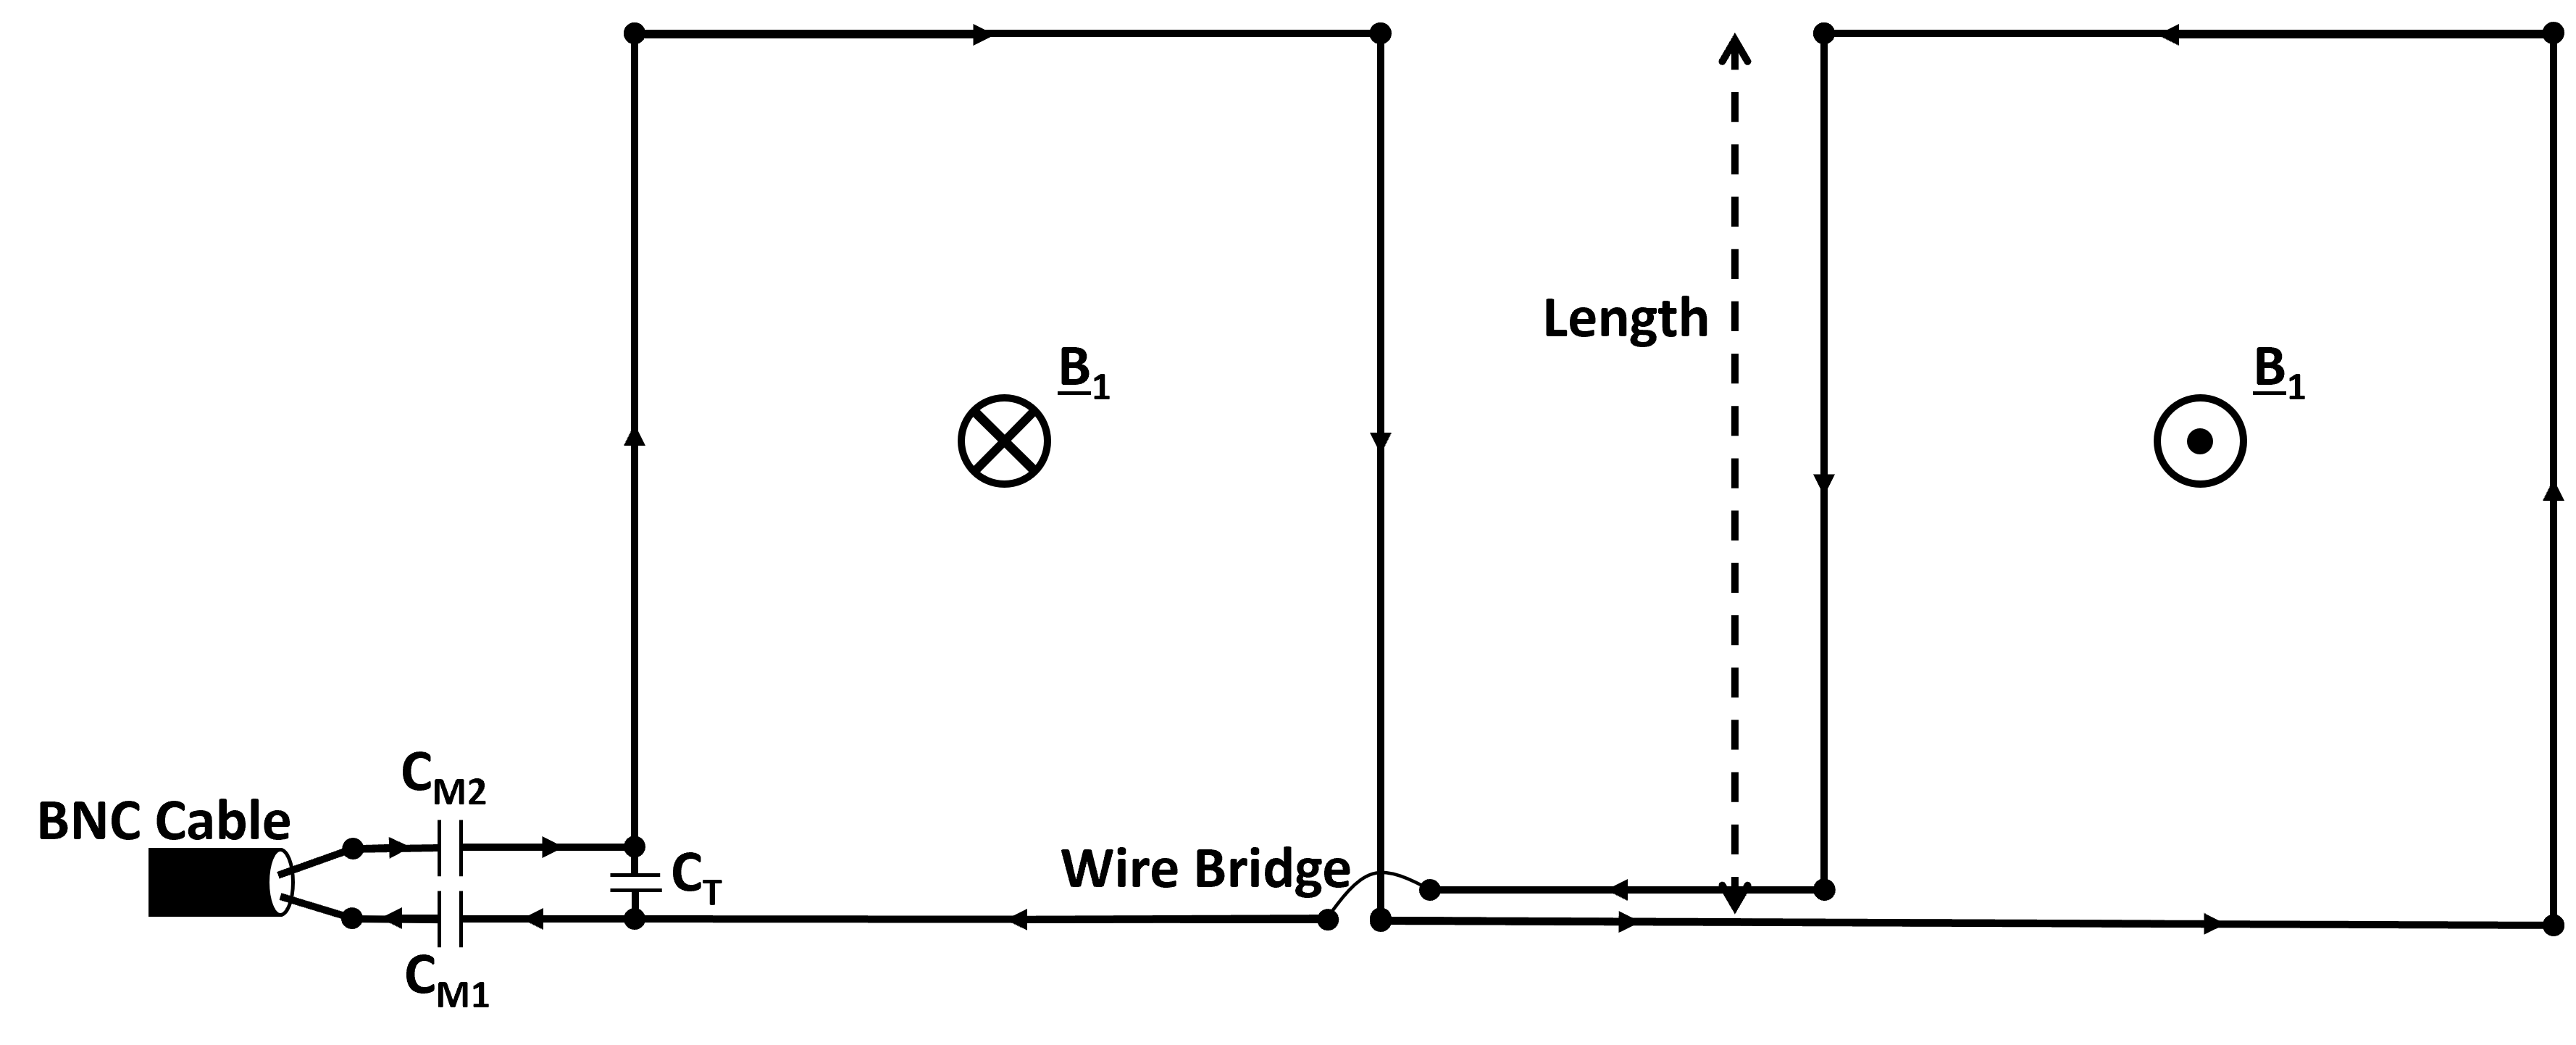
\includegraphics[width=1\textwidth]{Figures/Theory/Planar_Saddle.png}
    \caption{\textit{2D circuit diagram of the saddle coil used for scanning of the calf.}}
    \label{fig:theory:2D_Saddle}
\end{figure}

Volumetric coils such as saddle coils have much more homogeneous B$_1$ fields than surface coils and are able to cover a much larger volume. A saddle coil is derives its name from the fact it has a similar appearance to a horse's saddle, two square loops surround a circular tube with an angular separation. The saddle coil has optimum geometry that has been previously been found which includes the length/diameter between 1 and 2, and an angular width for each coil of $\approx$120$^\circ$ \cite{Ginsberg1970OptimumField,Salmon2006OptimizationImaging}.

\begin{figure}
    \centering
    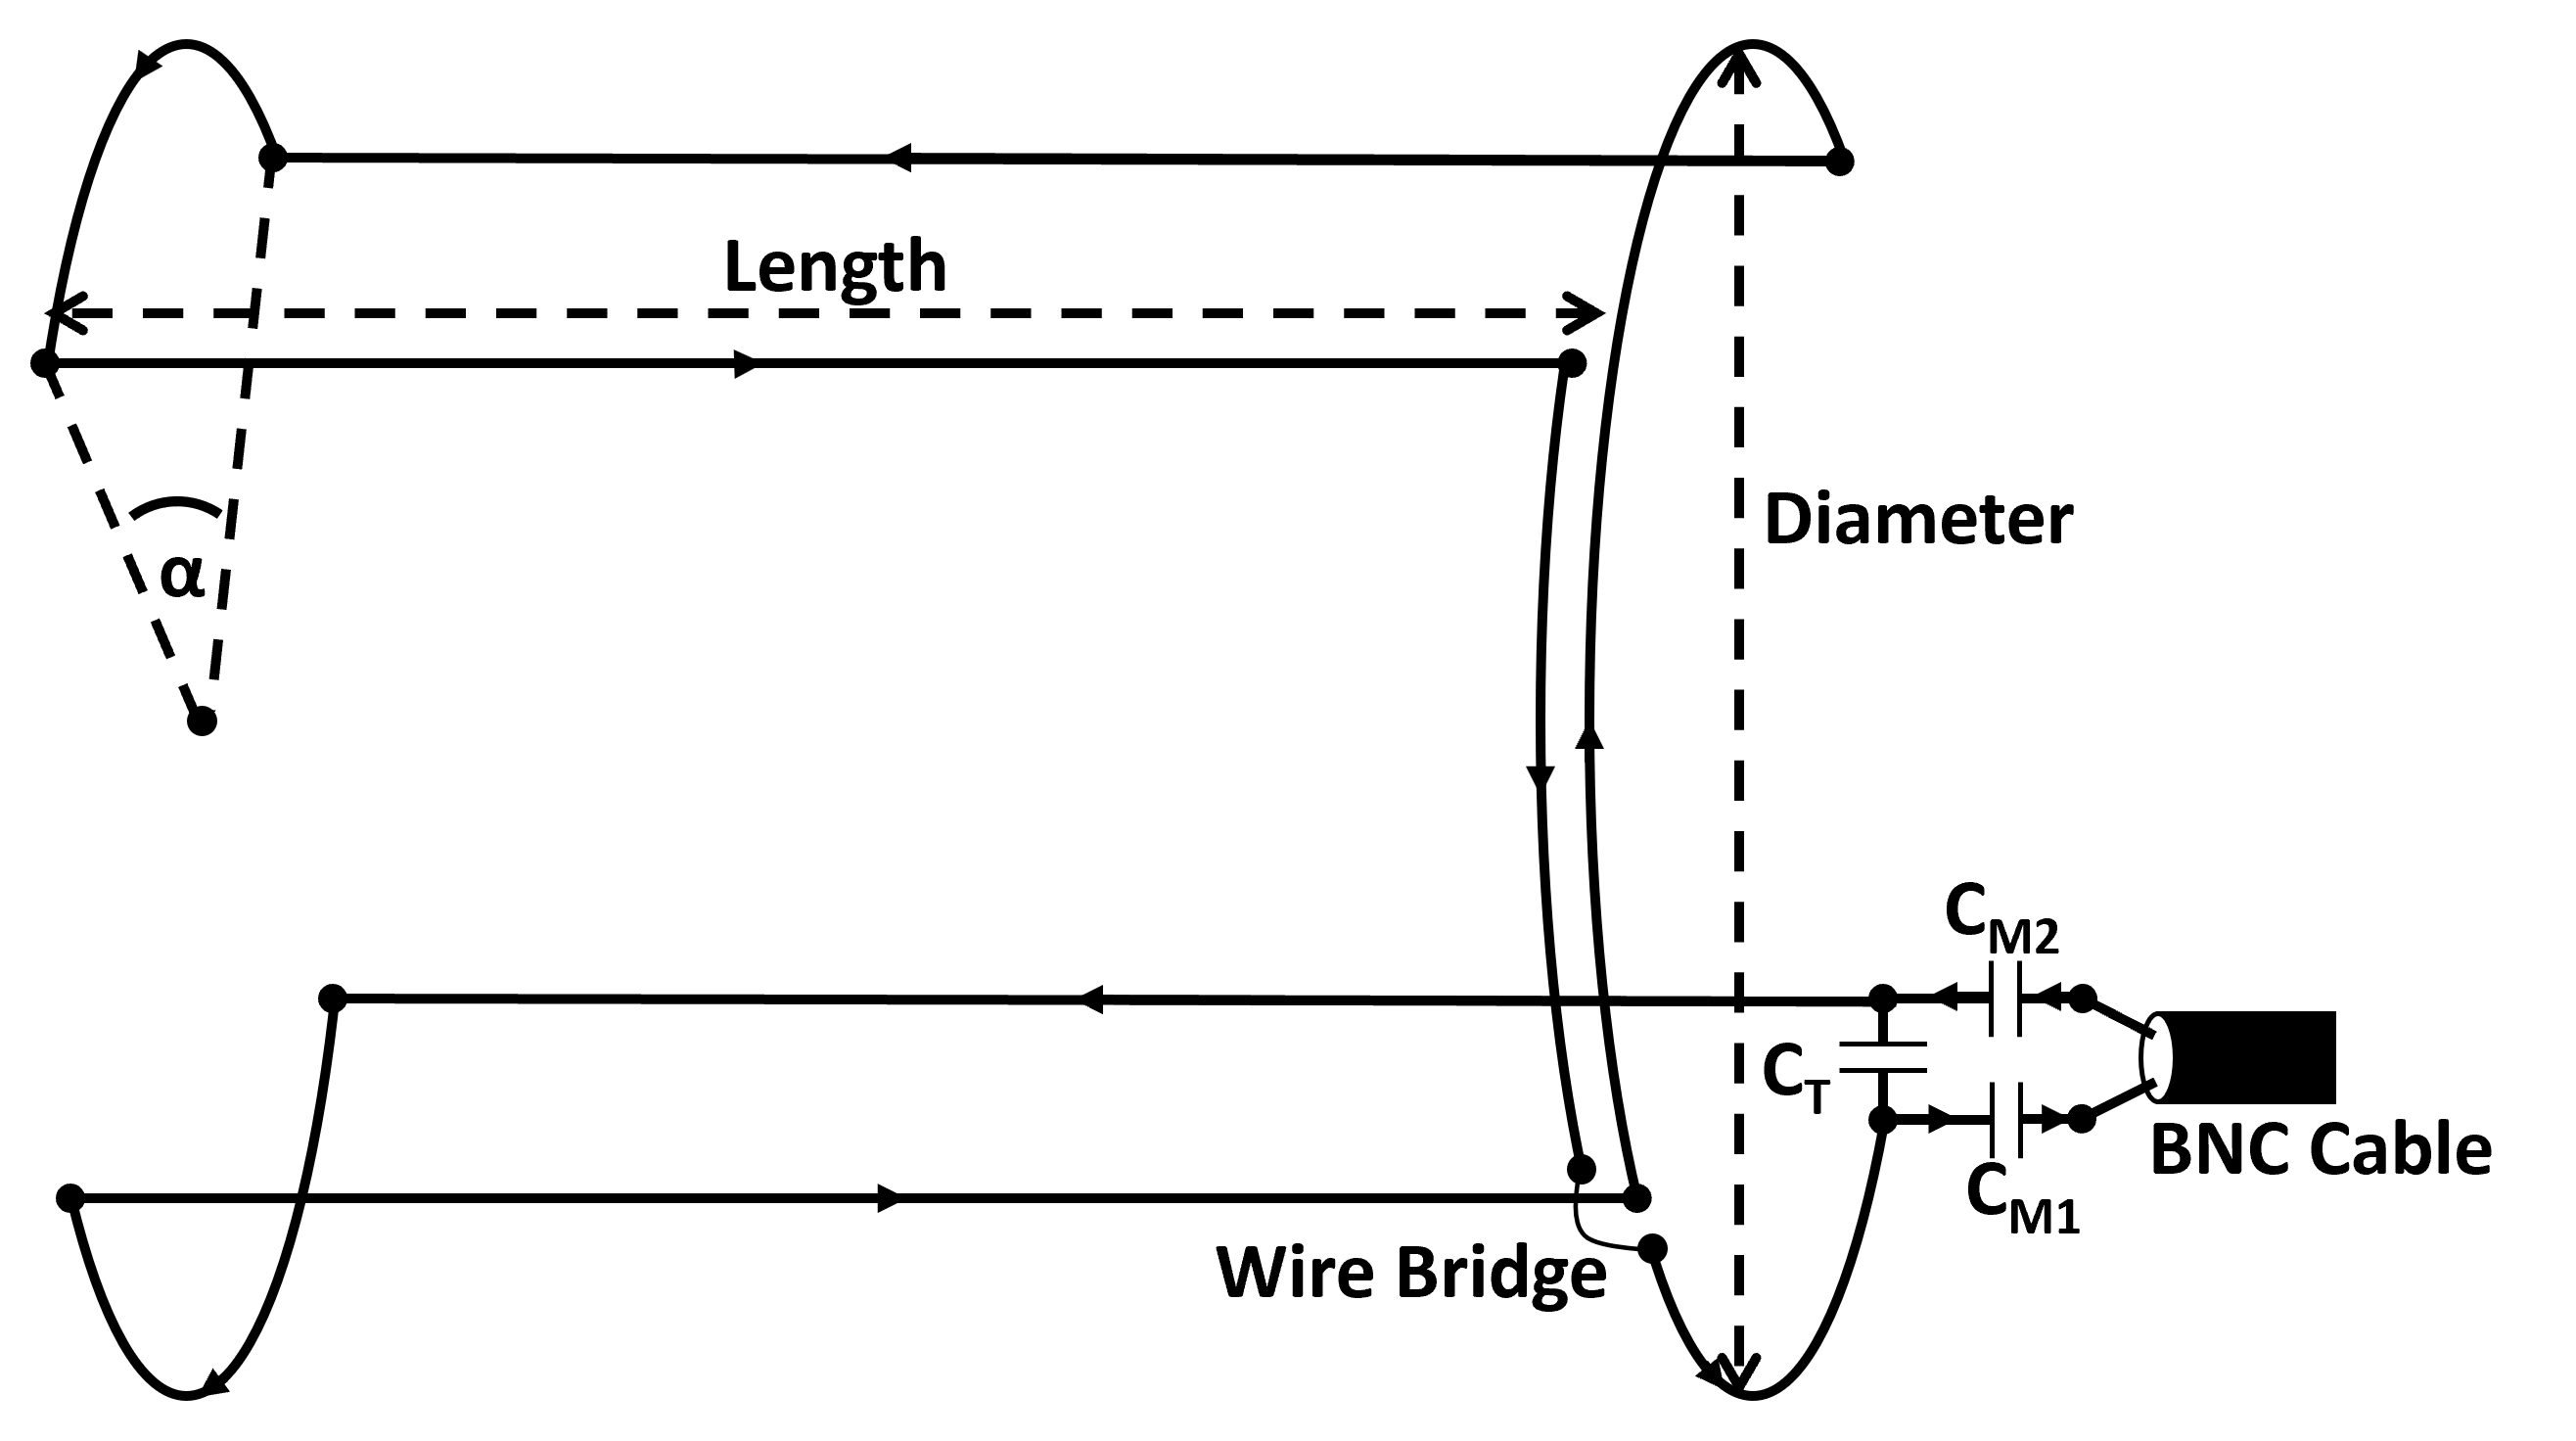
\includegraphics[width=0.8\textwidth]{Figures/Theory/3D_Saddle.png}
    \caption{\textit{3D circuit diagram of the saddle coil used for scanning of the calf.}}
    \label{fig:theory:3D_Saddle}
\end{figure}

The coil built for scanning in Chapter \ref{Chap:Quad} is made from copper tape and has an angular width of 120$^\circ$ a length of 16.8 cm and a diameter of 14.8 cm. Where the copper tape that links the two squares intersects/crosses over an insulated wire is used to avoid a capacitor being created. Also, the wires here run close side by side so that the fields from the opposing currents will cancel. Diagrams of the circuit for the coil are shown in figures \ref{fig:theory:2D_Saddle} and \ref{fig:theory:3D_Saddle} with pictures in Figure \ref{fig:theory:Saddle_pic}. The tuning capacitance is 47.3 pF, the total matching capcitance 8.8 pF.

\begin{figure}
    \centering
    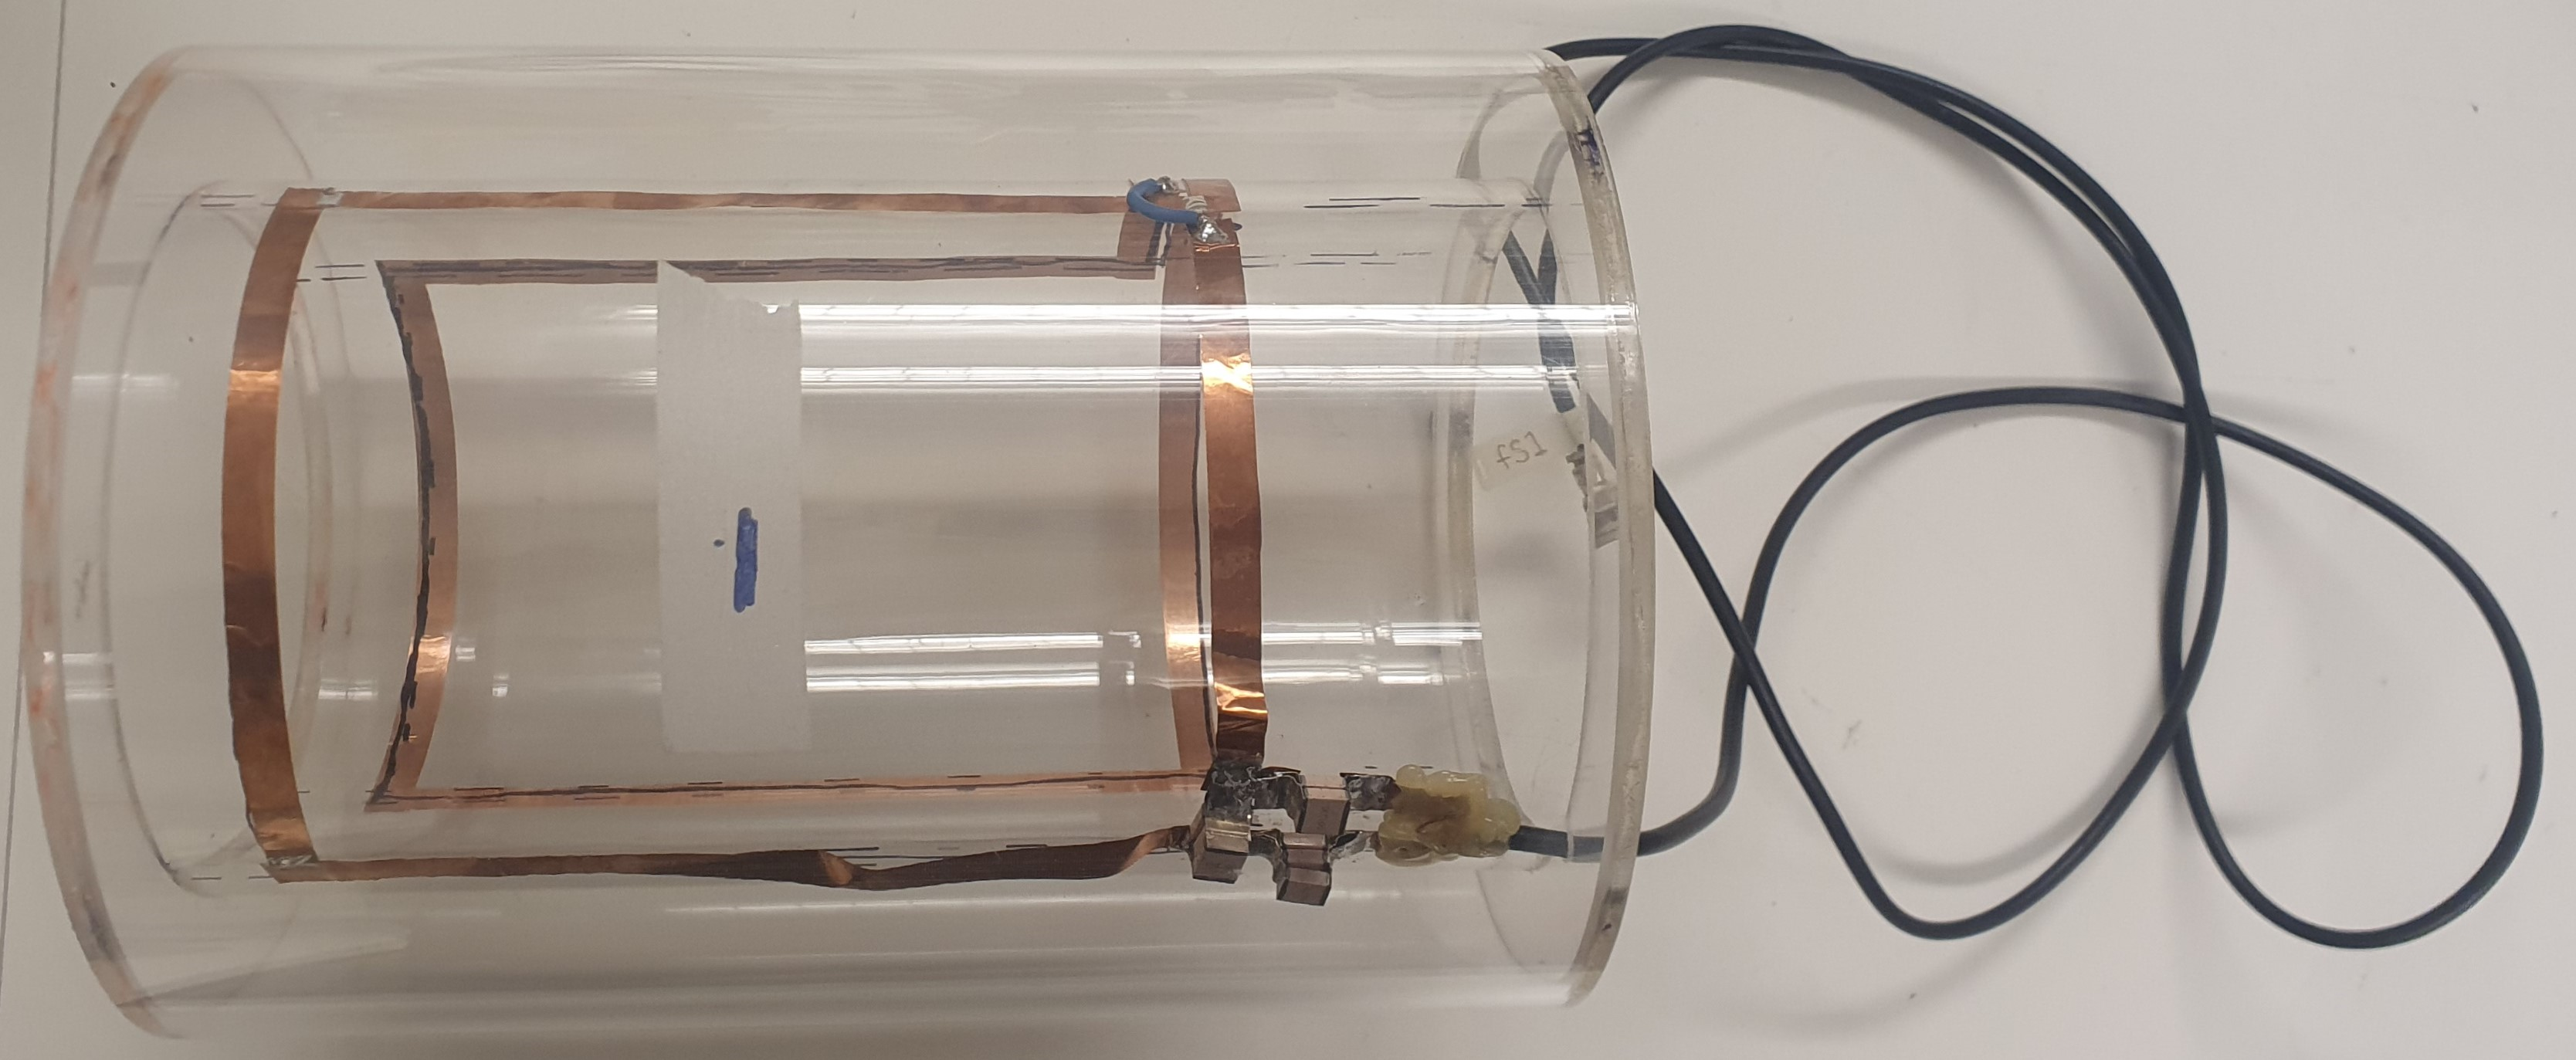
\includegraphics[width=1\textwidth]{Figures/Theory/Saddle_Coil.jpg}
    \caption{\textit{Photo of the saddle coil used to obtain $^2$H data from the calf.}}
    \label{fig:theory:Saddle_pic}
\end{figure}

\subsubsection{Helmholtz coil}

\begin{figure}
    \centering
    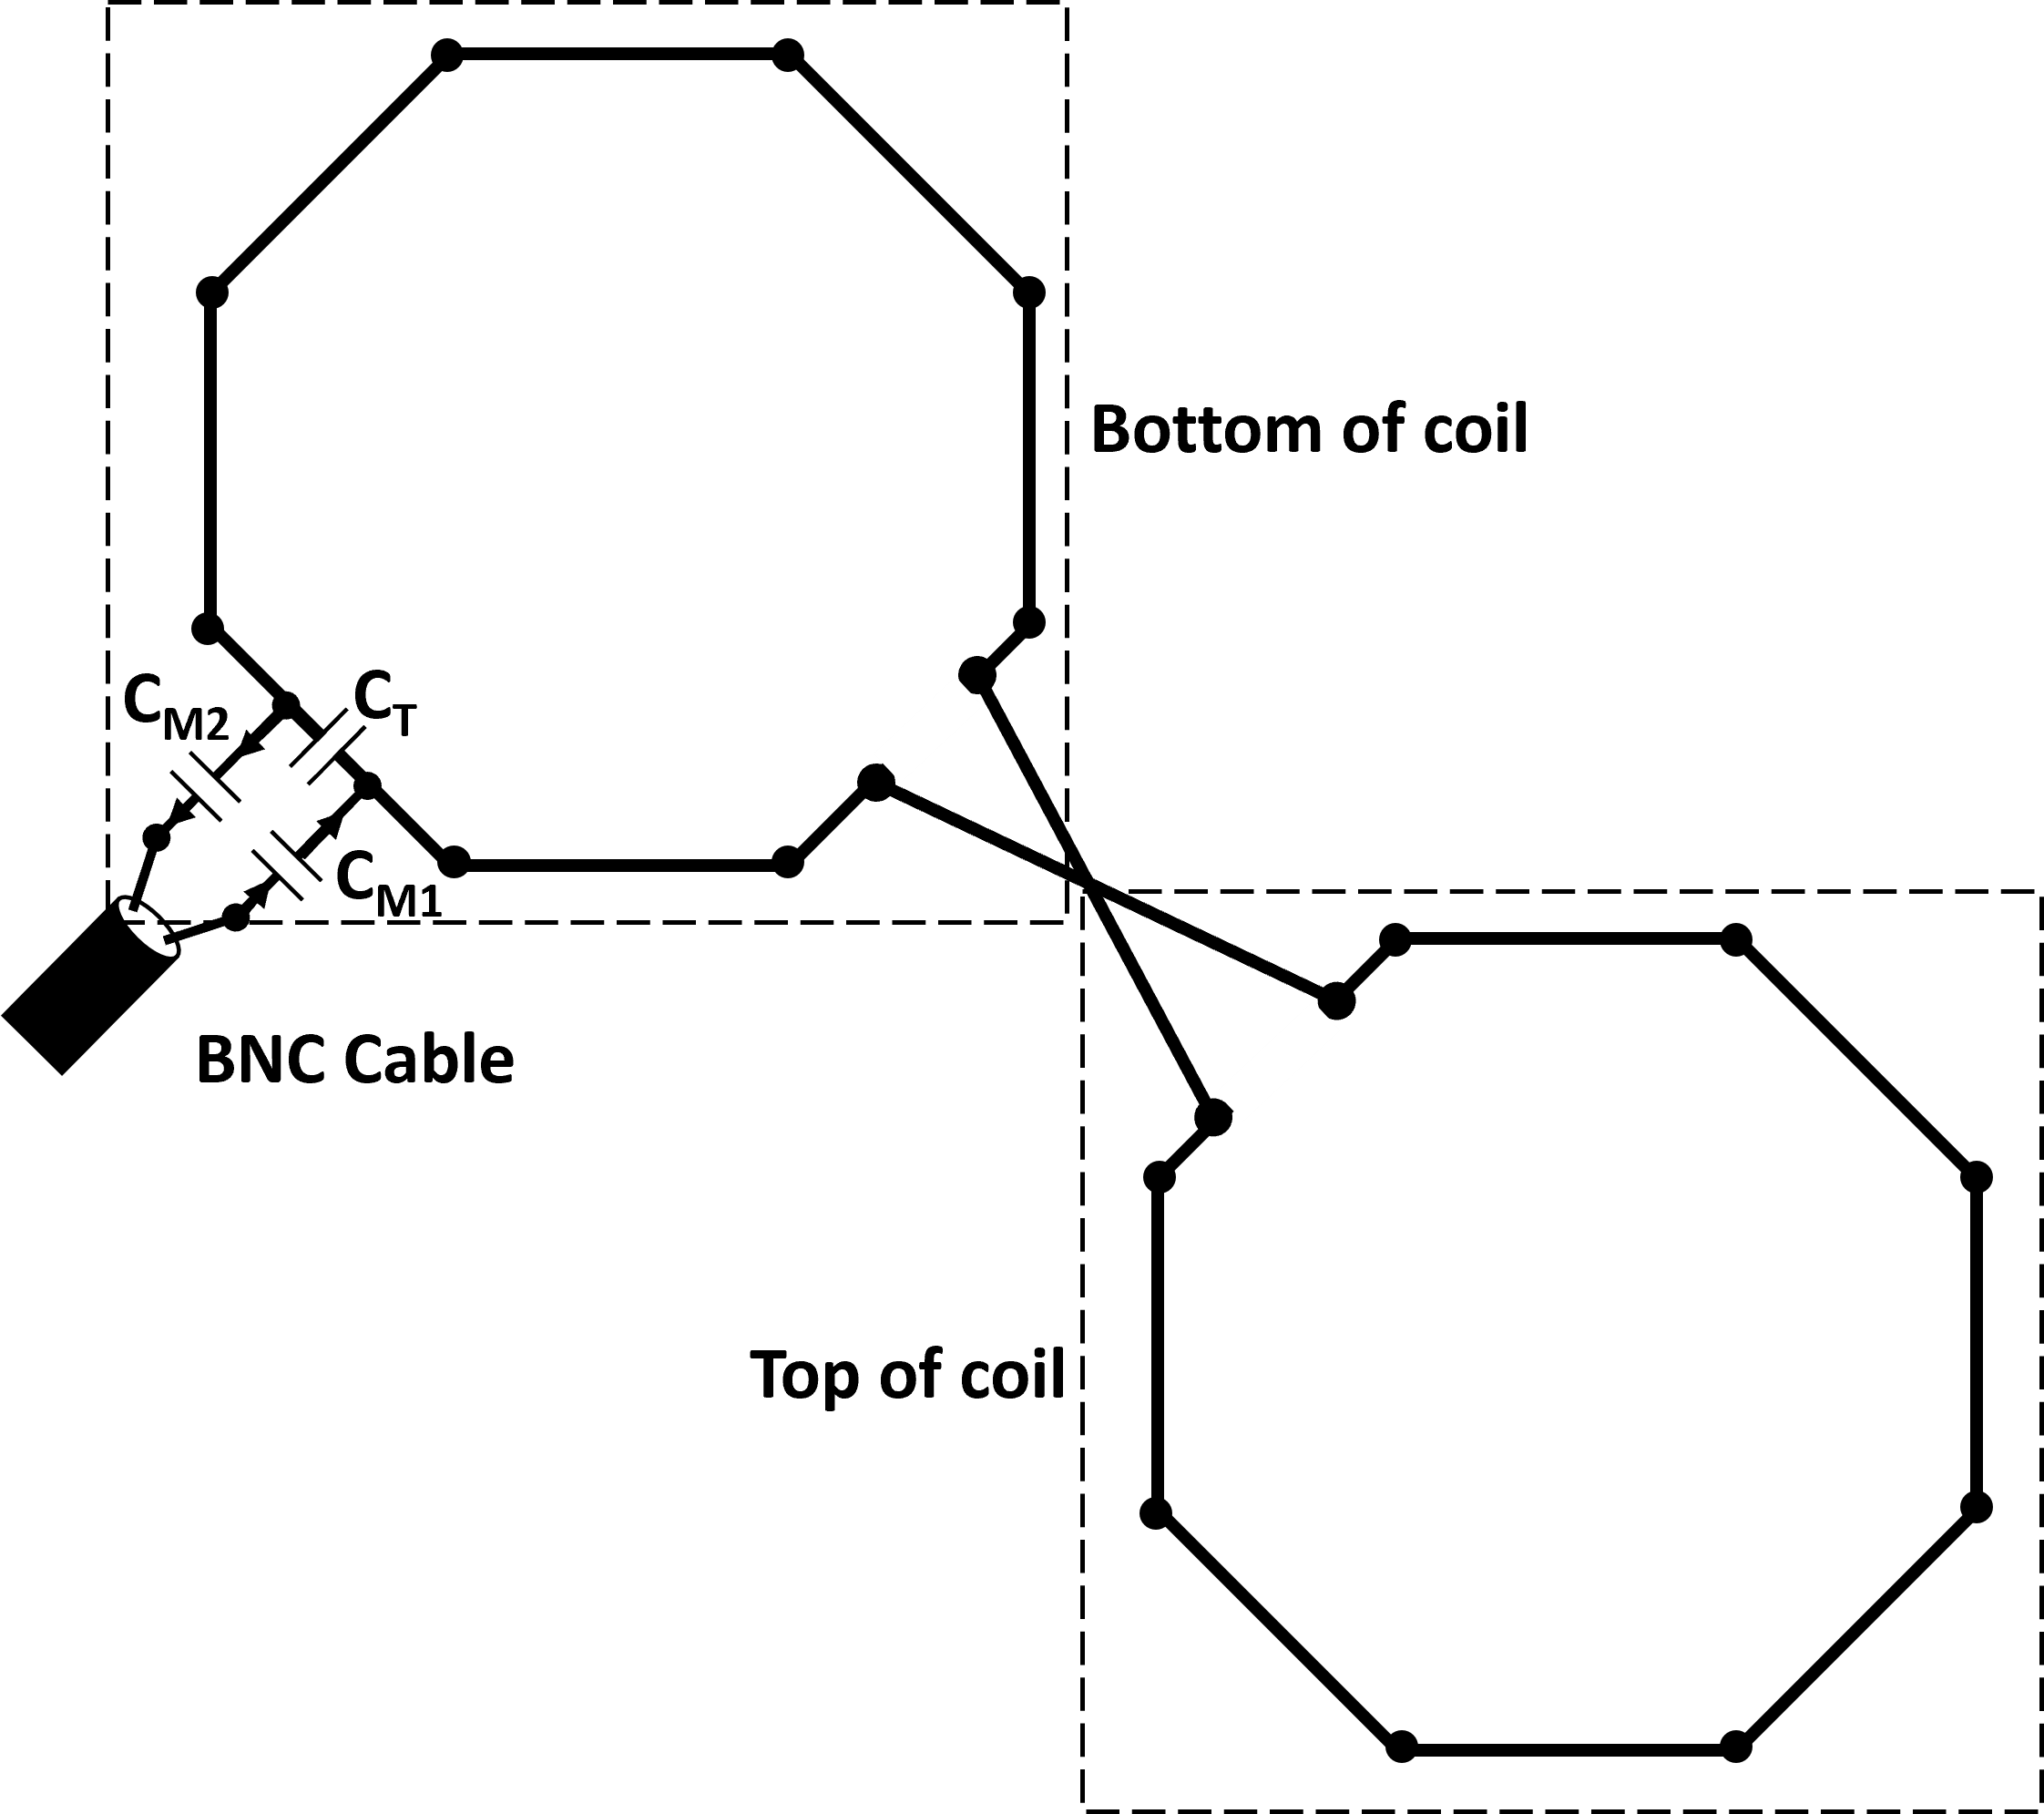
\includegraphics[width=0.8\textwidth]{Figures/Theory/Planar_Helmholtz.png}
    \caption{\textit{2D circuit diagram of the Helmholtz coil used for scanning of the arm.}}
    \label{fig:theory:2D_Helmholtz}
\end{figure}

A Helmholtz coil is similar to to a surface coil in its circuitry. Except a second surface coil is connected to it by two crossing insulated wires, where the current in each flows in opposite directions so that the field flows in the centre of the setup. This creates a homogeneous B$_1$ in between the coils. The Helmholtz coil arrangement was chosen as the scanning is of the arm and needs to be easily movable and a saddle coil would roll/move to much and would be difficult to rotate in the magnet bore.

\begin{figure}
    \centering
    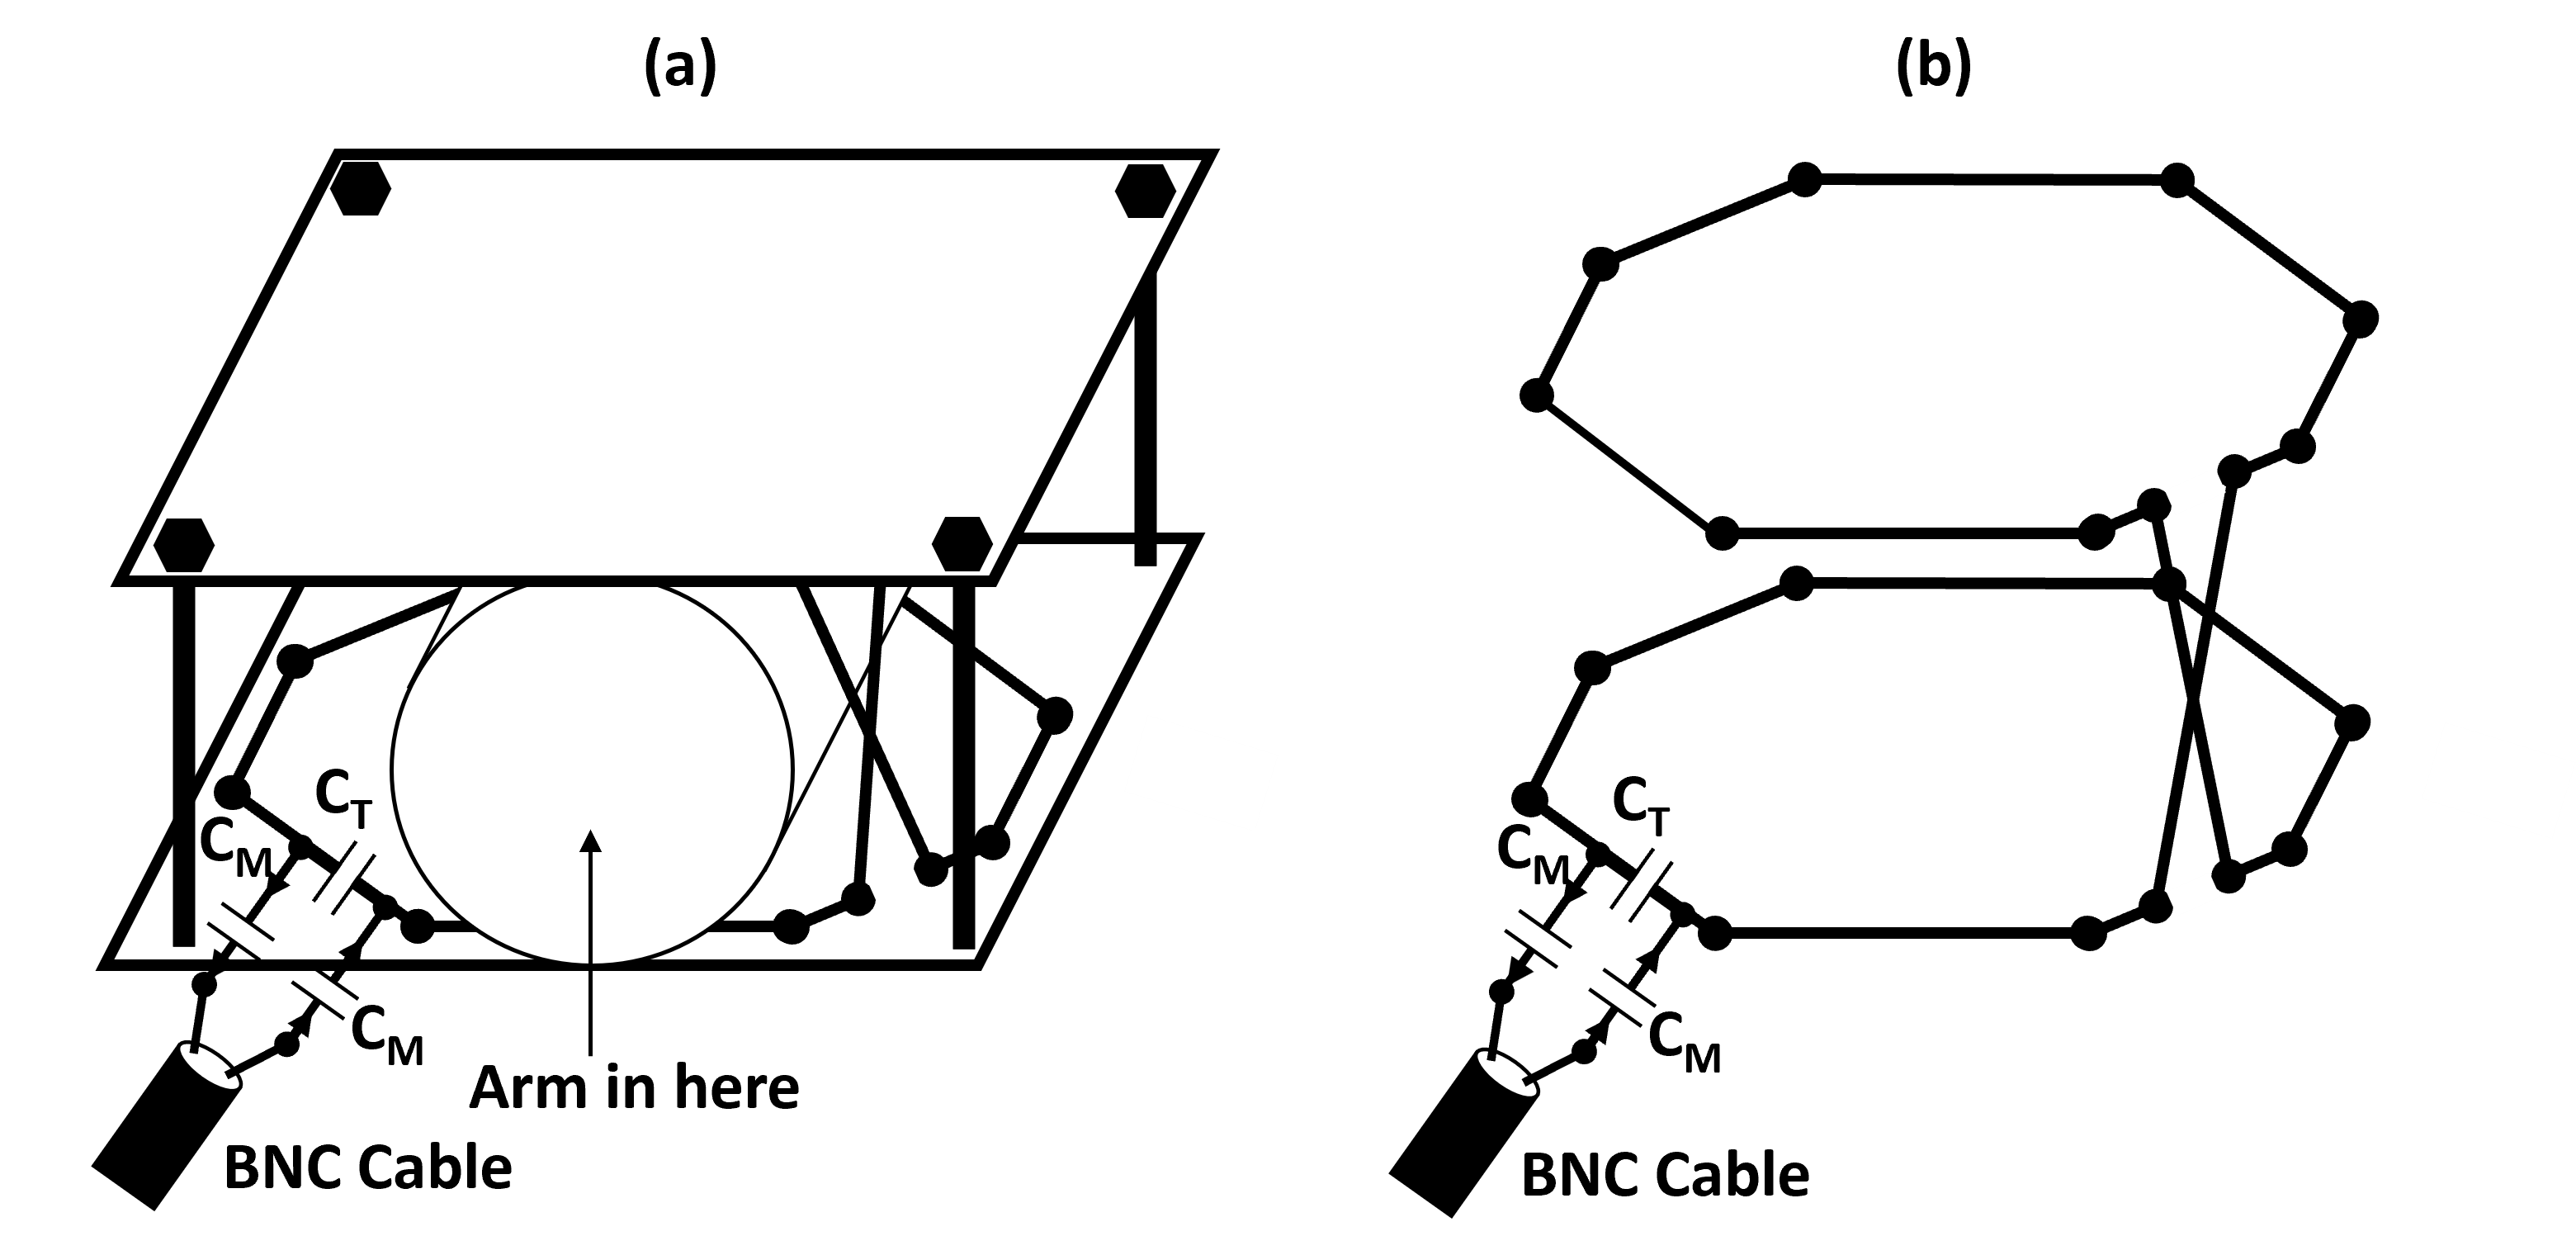
\includegraphics[width=1\textwidth]{Figures/Theory/3D_Helmholtz.png}
    \caption{\textit{3D circuit diagram of the Helmholtz coil used for scanning of the arm with housing (a) and without (b).}}
    \label{fig:theory:3D_Helmholtz}
\end{figure}

The coil setup involves two octagonal loops that are $\approx$14 cm in diameter separated by a 12 cm gap with a tube in the centre to keep the arm in the same position, still and away from the circuit elements. The Tuning capacitance is 73.3 pF and the total matching capacitance is 8.8 pF.

\begin{figure}
    \centering
    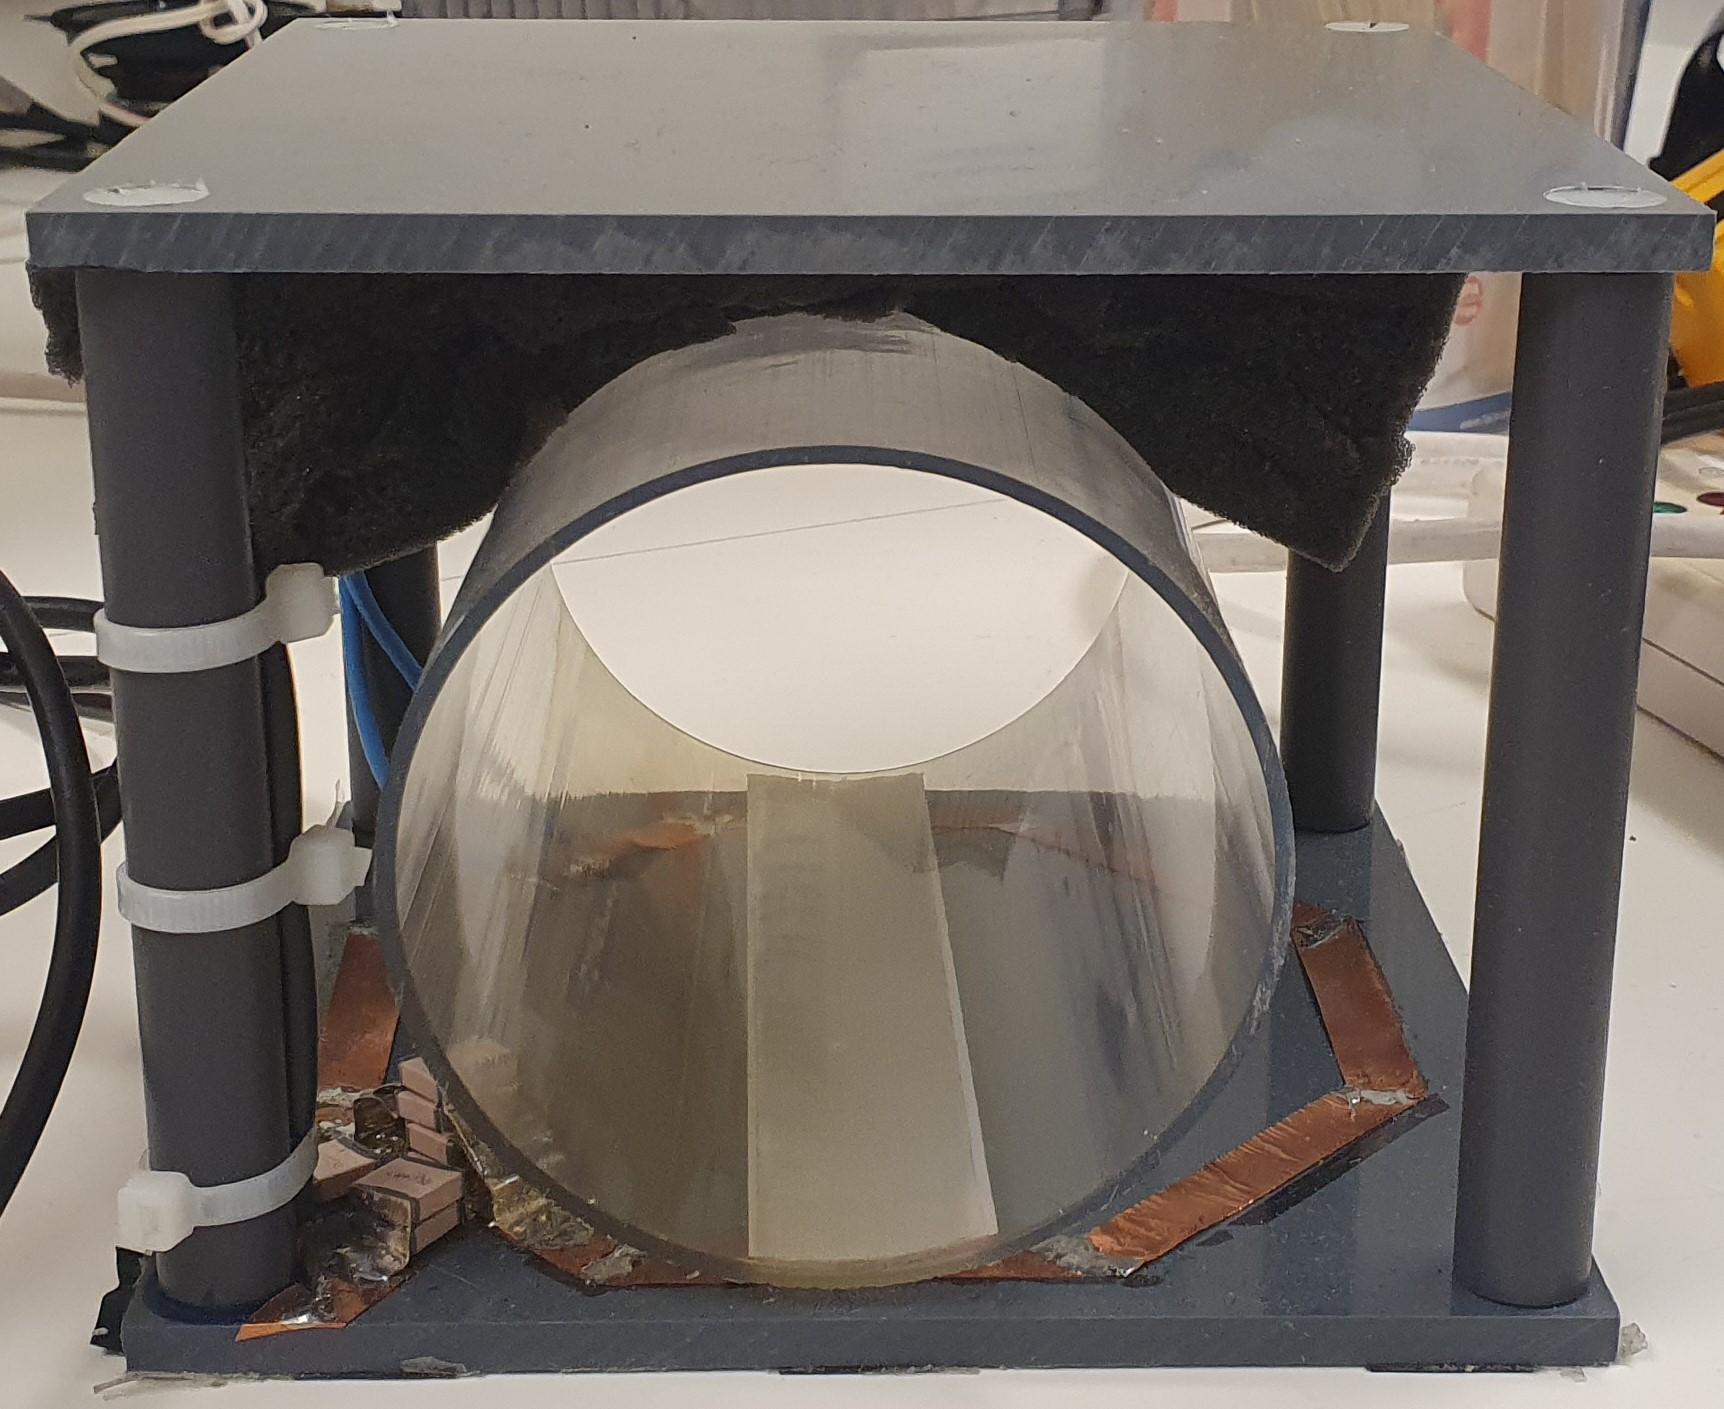
\includegraphics[width=0.8\textwidth]{Figures/Theory/HelmHoltz_Coil.jpg}
    \caption{\textit{Photo of the HelmHoltz coil used to obtain $^2$H data from the arm.}}
    \label{fig:theory:HelmHoltz_pic}
\end{figure}